%\documentclass[a4paper,12pt,oneside,draft]{report}
\documentclass[a4,12pt,fullpage]{report}
%\setpapersize{A4}
%\usepackage{a4}
%\usepackage{lscape} % in latex preamble
\usepackage{amssymb,graphicx, rotating, epstopdf}
\usepackage{epsfig,amsmath,amsfonts}
\usepackage{float}
\usepackage[english]{babel}
\usepackage{subfigure}
\usepackage{vmargin}
\usepackage{textcomp}
\usepackage{notebook}
\usepackage{setspace}
\usepackage{pxfonts}
\usepackage{booktabs}
\usepackage{mathtools}
\usepackage{amsmath}
\usepackage{amssymb}
\usepackage{cancel}
\usepackage{subfigure}
\usepackage[export]{adjustbox}
    \usepackage{wrapfig, framed,multicol}
    \usepackage{lipsum}
    \usepackage{filecontents}
    \usepackage[numbered,framed]{matlab-prettifier}%

        % Line spacing
%\setmargins{3.5cm}{3.5cm}{14cm}{20cm}{0pt}{2cm}{0pt}{3cm}
%\setmargins{2.5cm}{2.5cm}{16cm}{22cm}{0pt}{1cm}{0pt}{2cm}
%\usepackage{showkeys}
\usepackage{fancyhdr}
%\pagestyle{fancy}
%\lhead{\nouppercase{\leftmark}}
%\chead{}
%\rhead{\thepage}
%\lfoot{}
\newtheorem{thm}{Theorem}[section]
\newtheorem{definition}{Definition}[section]
\newtheorem{remark}{Remark}[section]
\newtheorem{proof}{Proof}[section]
\newtheorem{example}{Example}[section]
\newtheorem{lemma}{Lemma}[section]
%\newtheorem{property}[thm]{Property}
%\definition{def}{Definition}[chapter]
%\cfoot{\thepage}
%\rfoot{}
\topmargin 1cm
\oddsidemargin 2cm
\evensidemargin 2cm
\textwidth 16.59cm
\textheight 21.94cm
\renewcommand{\baselinestretch}{0.5}


%%%%%%%%%%%%%%%%%%%%%%%%%%%%%%%   LAYOUT OF THE THESIS %%%%%%%%%%%%%%%%%%%%%%%%%%
%\input{thesis_layout.tex}
%%%%%%%%%%%%%%%%%%%%%%%%%%%%%%%%% NEW DEFINITIONS       %%%%%%%%%%%%%%%%%%%%%%%%%
%%%%%%%%%%%%%%%%%%%%%%%%%%%%%%%%% MAIN DOCUMENT %%%%%%%%%%%%%%%%%%%%%%%%%%%%%%%%%
%\includeonly{section2}
%\includeonly{ch4}
\begin{document}

%\onehalfspacing

%\noindent
%%%%%%%%%%%%%%%%%%%%%%%%%%%%%%%%% TITLE PAGE %%%%%%%%%%%%%%%%%%%%%%%%%%%%%%%%%%%%
%\pagenumbering{roman}
%\setcounter{page}{1}
%\thispagestyle{empty}
\thispagestyle{empty}
\begin{center}
\vspace*{1cm}
{\huge Numerical Simulations for Selected 1D and 2D Mass Spring Models and Applications }

\vspace*{1.5cm}
\large { for the Bachelor of Science (General) Degree \\By\\E.S.K.Chandrasekara\\Sc/2018/10559}\\
\vspace{1.3cm}
\large {Supervisor:\\ Dr. M.K. Abeyratne }\\
\vspace{1.9cm}
%\date{Date}
\large{Department of Mathematics}\\
\large{University of Ruhuna}\\
\large{Matara.}\\
\vspace{0.5cm}
\large{2022}
\end{center}





\pagenumbering{roman}
\setcounter{page}{1}
%\newpage
%%%%%%%%%%%%%%%%%%%%%%%%%%%%%%%% ACKNOWLEDGEMENTS ABSTRACT etc.%%%%%%%%%%%%%%%%%%
%\thispagestyle{empty}
\include{dec}
%\noindent
%\newpage
%%%%%%%%%%%%%%%%%%%%%%%%%%%%%%%%  MAIN CHAPTERS %%%%%%%%%%%%%%%%%%%%%%%%%%%%%%%%%
\chapter*{Acknowledgment}
\paragraph{}
 
This project becomes a reality with the kind support and help of many individuals. I would like to extend my sincere thanks to all of them.

First, I would like to express my deepest gratitude to my supervisor, Dr.M.K.Abeyratne for his continuous contribution and supervision throughout the completion of this project which was invaluable.

I am immensely thankful to Dr.W.M.K. De Silva of the Department of Physics for providing related details which helped me to complete this project.

Besides my supervisor, I wish to thank Dr.B.G. Sampath A. Pradeep for conducting previous lectures and offering us Matlab programming opportunities. Without her passionate participation,
this project could not have been successfully conducted.

I am also thankful to all academic staff members of the Department of Mathematics of the Faculty of Science University of Ruhuna for their kind advice.

An extra special thank you to my group members, who were simply the greatest. 


\chapter*{Abstract}
\paragraph{}

The vibration phenomenon can be noticed in many common settings, including speaking, vision, auditioning, and other activities involving human relationships due to mechanical waves. This phenomena is also required in various engineering applications related to our daily lives, where vibration is exploited to increase the comfort of various human activities. Because of their complexities, vibrations are difficult to characterize and estimate quantitatively. Despite the development of several mathematical models, it remains challenging to balance computational complexity and estimate the accuracy without a numerical analysis. This project focuses on adding physical accuracy and visual authenticity to existing one dimensional (1D) and two dimensional (2D) mass-spring models based on numerical analysis. The Lagrangian approach was used to obtain the motion of connected oscillator systems in both 1D and 2D. MATLAB demonstrates that the numerical process of the Runge Kutta fourth-order method is more computationally efficient. Firstly, the 1D mass-spring model parameters for the two degree of freedom (2DOF) are determined using various conditions. Interestingly, with the same mass and spring stiffness, it is demonstrated that the 1D mass-spring model has accurate resistance to lateral displacement characteristics, which is one of the most vital aspects of the accuracy of the 1D mass-spring model. Consequently, in the case of the imaginary frequency, there would be energy leakage, which defies the system's energy conservation criterion. In fact, the mass ratio $\mu$ should be greater than zero. The procedure is then extended to the 2D mass-spring model, where the mass $m$ could indeed move freely in the $XY$ plane. Isotope oscillations could be noticed in the 2D mass-spring model with varying phase difference values ($\Delta = 0 , \pi/4 , \pi/2$  and $3\pi/4 $). Since this angular frequency of oscillation in the $X$-direction is equal to the angular frequency of motion in the $Y$-direction, the particle's path would be a closed trajectory. The particle observed in the trajectory is called an anisotropic oscillation when $\omega_x = 2\omega_y$ and $\omega_x = \sqrt{2}\omega_y$. The accuracy and behaviour of mass-spring models were tested numerically under various scenarios to illustrate the efficacy of our technique.






































































































































































































































































%\renewcommand{\contentsname}{Contents}  % Original name = Contents
%\chapter*{Acknowledgment}
\paragraph{}
 
This project becomes a reality with the kind support and help of many individuals. I would like to extend my sincere thanks to all of them.

First, I would like to express my deepest gratitude to my supervisor, Dr.M.K.Abeyratne for his continuous contribution and supervision throughout the completion of this project which was invaluable.

I am immensely thankful to Dr.W.M.K. De Silva of the Department of Physics for providing related details which helped me to complete this project.

Besides my supervisor, I wish to thank Dr.B.G. Sampath A. Pradeep for conducting previous lectures and offering us Matlab programming opportunities. Without her passionate participation,
this project could not have been successfully conducted.

I am also thankful to all academic staff members of the Department of Mathematics of the Faculty of Science University of Ruhuna for their kind advice.

An extra special thank you to my group members, who were simply the greatest. 


%\begin{spacing}{1.5} % Environment for 1.2 line spacing for contents and lists
\tableofcontents
\newpage
%\cleardoublepage
%\end{spacing}
%\begin{spacing}{1.2}
\listoftables
\newpage
\listoffigures
%\cleardoublepage
%\end{spacing}
\newpage
%\addcontentsline{toc}{chapter}{Introduction}
\pagenumbering{arabic}
\setcounter{page}{1}
%\input{chap0.tex}
%\include{Ch2.tex}
 %\chapter{Introduction}
\label{chap:01}


\paragraph{}
The vibration phenomenon can be observed in various standard settings, including speaking, vision, auditioning, and other activities involving human interaction owing to mechanical waves and digital communication via electromagnetic waves \cite{tse1963mechanical}. Also, Vibrations are a part of our everyday lives, and individuals encounter them in various ways. This phenomenon is required in various engineering applications, such as car suspension, where vibration increases driver comfort. They range from small-scale motions of atoms in substances to large-scale swaying of buildings and other structures and can be welcomed and intended, or bothersome and, in the worst case, harmful \cite{mori2017mechanical}. Oscillatory motion is joint, and physicists frequently idealise these examples of vibration into instances of a beneficial fiction, the harmonic oscillator. 

A mathematical depiction of a physical, biological, or information system is a simulation \cite{wada1972equivalent}. Models enable us to think about a system and forecast its behaviour. A dynamical system is one in which the consequences of actions do not arise instantly. For example, a headache does not go away immediately after taking aspirin; it takes time to take action. Additional funding for a development project does not enhance profits in the short term, but it may do the same in the longer - term in enterprise applications. All of these are instances of dynamical systems, in which the system's behaviour varies through time. As previously stated, the mass-spring model has been widely utilised to simulate deformable objects for facial animation \cite{keeve1998deformable}, animation of artificial animals \cite{tu1994artificial}, cloth draping \cite{ji2006three}, garment animation \cite{provot1995deformation}, and, more recently, surgical simulations \cite{sorensen2007virtual}. Recent enhancements to this model include the inverse dynamics approach to eliminate super elongation of the springs \cite{mozafary2016study} and the implicit integration method to take substantial time steps. 


The mass-spring model can be considered a discrete approximation method for solving the Lagrange partial differential equation of motion \cite{baleanu2020new}. Because of the extreme discretisation, the mass-spring model will only approximate the continuous object in some ways. The mass-spring model and the finite element method (FEM) \cite{duan2014volume} were compared, and it was determined that an exact simulation using the mass-spring model is unattainable. This project could clarify why there hasn't been much research on optimising the parameters of the mass-spring model. Even though the mass-spring model cannot provide an exact simulation, certain reasonable parameter sets provide more physically realistic simulations than others. The mass-spring model is currently implemented using a trial-and-error approach to determine parameter values for many applications. Aside from the fact that the criteria are highly subjective, the process is extremely laborious and time-consuming.

The capacity to forecast and reduce structural vibrations has recently attracted more attention. Vibrations originate from either external sources, such as wind, or internal sources, including friction between mechanical pieces of a system. The most typical scenario of vibration is break squeal in automobiles \cite{suggs1969application}. As a result, researchers have focused their efforts on studying vibration phenomena and their applicability in real life \cite{levitan1960forced} \cite{pellicer2004analysis} \cite{grandmont2006viscoelastic}. Because their occurrence is inherently dependent on the unique internal properties, the motion can be described mathematically as the unstable homogeneous solution to the homogeneous equations of motion. Furthermore, mathematical solutions will be discussed in detail in future chapters. 

\section{Background of the study}
\label{sec:1.1}

\paragraph{}

The study of linked oscillators has since become an important branch of mathematics, with applications in physics, biology, and chemistry \cite{Chapter427:online}. Coupled oscillators are seen in biological systems as well \cite{winfree1967biological} \cite{hannay2018macroscopic}. Most species directly correspond to numerous patterns in our environment, such as the earth's rotation around the sun, the alternation of night and day, or the tides. Organisms demonstrate periodicities due to their environment and exhibit innate periodic activity. Inhalation, blood circulation, chewing, molecular motion and galloping are all instances of rhythmic motion patterns. Waves are the propagation of oscillations in space caused by the connection of individual oscillators. A straightforward exercise is to strike the right piano note, which sounds the tuning-fork tuned to the same frequency as the key we hit. Another scenario is the powerful sound of the frequency corresponding to the resonance frequency of the glass breaking a delicate wine glass. In this section coupled oscillators, Degree of freedom, Euler's Lagrange, Runge kutta method (fourth order) and other relevant background will be discussed. 


\subsection{Coupled oscillators}

\paragraph{}

Like the small-amplitude swinging of a pendulum, some oscillations are extremely simple and can be approximated by a single mass on the end of a Hooke'slaw spring. And some are more complex but could still be represented by two or more masses and two or more springs. Examples are compound mechanical systems, oscillating electrical circuits with multiple branches, multi-atom molecules, and elastic materials.  Here we display the few example of coupled oscillators used to understand oscillations like these.

\subsubsection{Linear systems of masses and springs}
As shown in Figure \ref{fig:1}, the blocks are attached to three springs, and the outer springs are likewise attached to stationary walls. The outer springs each have a force constant $k$, while the inner spring has a force constant $k'$. When the blocks are at rest, the springs are untethered. Let $x_1$ and $x_2$ represent the displacements of blocks 1 and 2 from their equilibrium locations, positive to the right. Assume three blocks are connected to four springs: In the equilibrium position, the springs are again unstretched, and the blocks can only move horizontally. Each outer spring's far end is linked to a stationary wall. The three blocks' displacements from equilibrium are $x_1$,$x_2$, and $x_3$, all positive to the right. Assume the blocks have the same mass $m$ and the same force constant $k$, as shown in Figure \ref{fig:5}.


 \begin{figure}[hbt!]
	\centering
	\begin{framed}
	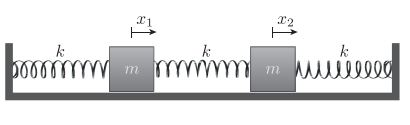
\includegraphics[width=0.6\textwidth]{Figures/A.JPG}
	\end{framed}
	\caption{Two blocks are attached to three springs \cite{Departme83:online}.}
	\label{fig:1}
\end{figure}

 \begin{figure}[hbt!]
	\centering
	\begin{framed}
	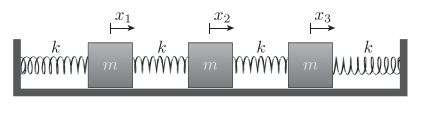
\includegraphics[width=0.6\textwidth]{Figures/E.JPG}
	\end{framed}
	\caption{Three blocks are attached to four springs \cite{Departme83:online}.}
	\label{fig:5}
\end{figure}

So far, we've only worked with masses attached to Hooke's law springs, which are, of course, highly idealised systems. More realistically, for macroscopic one dimensional mechanical motions here we concerned $CO_2$ molecules. As illustrated in Figure \ref{fig:4}, carbon dioxide is a linear molecule with the carbon atom (of mass m and coordinate x2) in the middle and the oxygen atoms (of mass M and coordinates x1 and x3) at the two ends. The behavior of the atoms at the scale of molecules is, of course, governed by quantum mechanics, and hence classical mechanics is merely a rough approximation to the true behaviour of the $CO_2$ molecule.

 \begin{figure}[hbt!]
	\centering
	\begin{framed}
	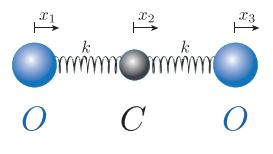
\includegraphics[width=0.35\textwidth]{Figures/D.JPG}
		\end{framed}
	\caption{The carbon dioxide molecule \cite{Departme83:online}.}
	\label{fig:4}
\end{figure}

\subsubsection{Coupled pendulums}

Two m-mass balls are tied to two equal-length $l$ strings to form side-by-side pendulums of equal period. As shown in Figure \ref{fig:2}, a weak spring $k$ is now coupled to the two balls. 

 \begin{figure}[hbt!]
	\centering
	\begin{framed}
	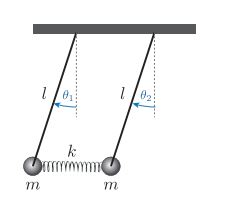
\includegraphics[width=0.38\textwidth]{Figures/B.JPG}
		\end{framed}
	\caption{Coupled pendulum \cite{Departme83:online}.}
	\label{fig:2}
\end{figure}

\subsubsection{ A planar system: masses in an equilateral triangle}

All particles and springs were aligned along a straight line and were only permitted to oscillate along that same straight line. Figure \ref{fig:3} depicts the normal-mode oscillations of a system with three equal masses $m$ and three equal springs $k$ in the shape of an equilateral triangle.

 \begin{figure}[hbt!]
	\centering
	\begin{framed}
	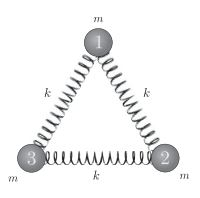
\includegraphics[width=0.33\textwidth]{Figures/C.JPG}
	\end{framed}
	\caption{Masses in an equilateral triangle
 \cite{Departme83:online}.}
	\label{fig:3}
\end{figure}

When a system is aroused into oscillations that are a mixture of normal modes \cite{cochelin20197th}, the motion will alter with time. Perhaps one of the masses will decrease amplitude and transfer energy to another mass, which will then return the energy \cite{kerschen2009nonlinear}. Even if the oscillations are all at the same frequency, such motion is totally distinguishable from simple harmonic motion and hence does not represent a normal mode. The transfer of energy usually occurs at a frequency that is significantly different from the frequency of oscillation.

\subsection{Degree of freedom}

\paragraph{}

Assume there are $N$ particles that can only move in one dimension. Then we define there seem to be N degrees of freedom (DOF) \cite{rosenberg1962normal}, $x_1, x_2,...x_N$, which are the positions observed along each particle's single dimension. If somehow the $N$ particles are instead permitted to travel in two dimensions, there are $2N$ degrees of freedom (DOF), $x_1, y_1,...x_N, y_N$, and so on. In case of that, Degrees of freedom (DOF) relate to the maximum number of logically independent values in a data sample, which are values with the freedom to fluctuate. DOF can be calculated using the below equation \eqref{1} and its corresponding constant values. 

\begin{equation}
    \label{1}
    DOF = (N \times n ) - k
\end{equation}

Where, \\
$n$ =  Number of dimensions \\
$N$ = Number of particles\\
$k$ = Number of constraints


\subsection{Euler-Lagrange equation}
\label{lag}

\paragraph{}

In this section, we'll learn about an entirely new way of seeing the world. Imagine the mass on the end of a spring. Of course, we can evaluate this by using $F = ma$ (Newton's second law) \cite{sharma2014isaac} to write out $m\Ddot{x} = k\Dot{x}$ \cite{zhong2019reliability}. As we all know, the solutions to such an equation are sinusoidal functions. However, we can sort things out by utilising a different strategy that does not reinforce F = ma. This new strategy is preferable to using Newton's second law in many (perhaps most) physical conditions. Here we now look at the lagrangian method. 

\begin{equation}
    \label{2}
    F_i = m\Ddot{x_i}
\end{equation}

The kinetic energy function, which is the time derivative of the momentum $p_1 = \partial T / \partial \Dot{x}$, determines the right side of this equation \eqref{2}. while the right hand side is a derivative of the potential energy, $- \partial U / \partial x_i$. . As $T$ is independent of $x_i$ and $U$ is independent of ˙$x_i$ in these coordinates, In terms of the Lagrangian, we can write both sides. 

\begin{equation}
    \label{3}
    L = T -U 
\end{equation}

Which is then a function of both the coordinates and their velocities. Thus we have established which will be known as Lagrange’s equation

\begin{equation}
    \label{4}
    \frac{d}{dt}(\frac{\partial L}{\partial \dot{xi}})-\frac{\partial L}{\partial xi} = 0 
\end{equation}

Here, $x = (x_1, . . . , x_N )$ and likewise $\dot{x}˙ = (\dot{x_1}, . . . , \dot{x_N})$. And also we can write \eqref{3} where
$T$ is the kinetic energy and $V$ is the potential energy. In the simplest cases, $T = T(\dot{x})$ and $V = V (x)$, The solution to a given mechanical problem is obtained by solving a set of $N$ second-order differential equations known as Euler-Lagrange equations of motion,

\begin{equation}
    \label{5}
    \frac{d}{dt}(\frac{\partial L}{\partial \dot{xi}})-\frac{\partial L}{\partial xi} = 0 
\end{equation}

\subsection{Numerical analysis}
\label{Num}

\paragraph{}
Numerical analysis is a branch of mathematics that teaches computer methods for studying and solving mathematical issues \cite{burden2015numerical}. In this section, we look at numerical approaches for solving the most frequent mathematical problems and analyse the errors that can occur while using these methods. Because practically all computation is now done on digital computers, we also explore the consequences for numerical method implementation.

The investigation of error is vital to numerical analysis. Most numerical approaches produce responses that are simply approximations to the intended genuine solution, and it is critical to understand the associated error and, if feasible, estimate or constrain it \cite{heydari2016theoretical}. This study looks at the numerous errors that can occur in a situation. The representation of numbers in computers, as well as the mistake in computer arithmetic, are investigated \cite{cui2018numerical}. The general results on the propagation of errors in calculations are presented, along with a detailed examination of errors in summing processes. Especially in this study, we will consider the Runge Kutta fourth-order (RK4) method \cite{islam2015accurate}. 

\subsubsection{Runge Kutta fourth order method}
\label{RK}
The fourth-order Runge-Kutta technique explains the lengthy computation of numerous unknowns, and the comprehensive step-by-step derivation and analysis can be found in many publications \cite{tan2012general} \cite{mehdi2017using}. Because of the method's importance in mathematics and applied science/engineering. By reviewing specific, possibly well-known papers, we simplify and minimise the complexity of their derivation and analysis by proposing a step-by-step derivation of the method.

In 1901, two German men, Carl Runge (1856-1927) and Martin Kutta (1867-1944), devised the Runge-Kutta Method \cite{tobies2012iris}. Carl Runge created numerical methods for solving the differential equations that evolved from his research on atomic spectra. These numerical techniques are still in use today. He employed so much mathematics in his studies that physicists mistook him for a mathematician, and he employed so much physics that mathematicians mistook him for a physicist. His name is now synonymous with the Runge-Kutta methods for numerically solving differential equations. Kutta, another German applied mathematician, is well recognised for his contribution to the Kutta-Joukowski theory of airfoil lift in aerodynamics, which is based on differential equations \cite{trefethen2015invented}. 

\newpage

\subsubsection{Runge-Kutta 4th order method to solve differential equation}

Given following inputs \cite{RungeKut7:online}. 

\begin{itemize}
    \item An ordinary differential equation that expresses the value of $dy/dt$ in terms of $t$ and $y$.
    \item Initial value of $y$, i.e., $y(0)$. 
\end{itemize}

\begin{equation}
    {{dy(t)} \over {dt}} = y'(t) = f(y(t),t), \quad \quad {\rm{with\;}} y(t_0)=y_0
\end{equation}

The evolution of the Fourth Order Runge-Kutta method closely parallels that of the second Order and will not be discussed in depth here. The fourth order method, like the second order method, has several variations that all employ four estimates to the slope. To determine the slope at some time t0 (assuming we just have an approximation to $y(t_0)$ (which we call $y^*(t_0)$), we will utilise the following slope approximations.

 \begin{figure}[hbt!]
	\centering
	\begin{framed}
	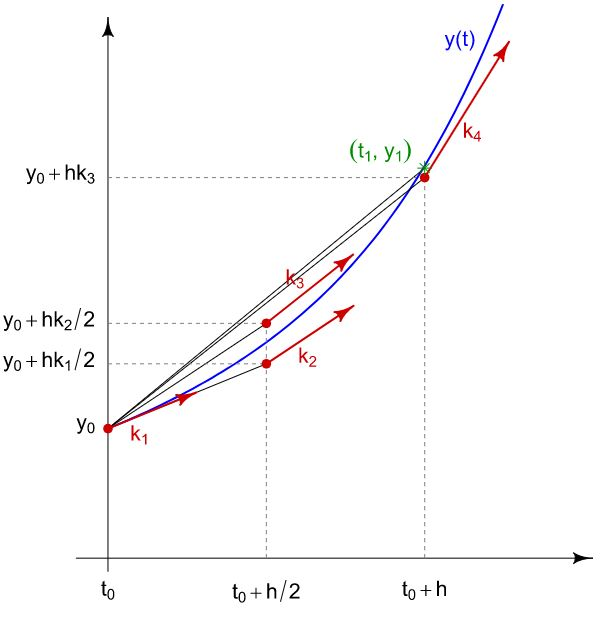
\includegraphics[width=0.6\textwidth]{Figures/F.JPG}
		\end{framed}
	\caption{Slopes used by the classical Runge-Kutta method \cite{hossain2017comparative}.}
	\label{fig:6}
\end{figure}

\newpage

\begin{equation}
    {k_1} = f({y^*}({t_0}),{t_0})
\end{equation}

\begin{equation}
    {k_2} = f\left( {{y^*}({t_0}) + {k_1}{h \over 2},{t_0} + {h \over 2}} \right)
\end{equation}

\begin{equation}
     {k_3} = f\left( {{y^*}({t_0}) + {k_2}{h \over 2},{t_0} + {h \over 2}} \right) 
\end{equation}

\begin{equation}
    {k_4} = f\left( {{y^*}({t_0}) + {k_3}h,{t_0} + h} \right)
\end{equation}

Each one of these slope estimates can be directly explained \cite{FourthOr20:online}.

\begin{itemize}
    \item $k_1$ is the slope at the beginning of the time step (this is the same as $k_1$ in the first and second order methods).
    
\item If we use the slope $k_1$ to step halfway through the time step, then $k_2$ is an estimate of the slope at the midpoint. This is the same as the slope$_2$, from the second order midpoint method. This slope proved to be more accurate than $k_1$ for making new approximations for y(t).

\item If we use the slope $k_2$ to step halfway through the time step, then $k_3$ is another estimate of the slope at the midpoint.

\item Finally, we use the slope, $k_3$, to step all the way across the time step$(t_0, t_0+h)$, and $k_4$ is an estimate of the slope at the endpoint. 
\end{itemize}

We then use a weighted sum of these slopes to get our final estimate of $y^*(t_0+h)$.

\begin{equation}
    {y^*}({t_0} + h) = {y^*}({t_0}) + {{{k_1} + 2{k_2} + 2{k_3} + {k_4}} \over 6}h 
\end{equation}



\begin{equation}
   {y^*}({t_0} + h) = {y^*}({t_0}) + \left( {{1 \over 6}{k_1} + {1 \over 3}{k_2} + {1 \over 3}{k_3} + {1 \over 6}{k_4}} \right)h
\end{equation}

\begin{equation}
   {y^*}({t_0} + h) =  {y^*}({t_0}) + mh
\end{equation}

 {\rm{where\;}}m{\rm{\;is\;a\;weighted\;average\; slope\; approximation.}}

The approach is comparable to the second order endpoint method \cite{dontchev2000second}, which employed an equal weighting of the slopes at the start and end of the interval. The weighting of the midpoint slopes ($k_2$ and $k_3$) is larger than that of the endpoint slopes ($k_1$ and $k_4$) in this case, because we expect these to be a better estimate of the slope while travelling from $y^*(t_0)$ to $y^*(t_0+h)$.


\newpage
\section{Problem statement and objectives}
\paragraph{}
Vibration analysis for frequency response and temporal response has become essential for significant industrial machines and other troubleshooting applications. The computation of natural frequencies for a finite coupled freedom system (one dimension and two dimension)  n-degree freedom system (one dimension and two dimension) and comparative amplitudes of vibrating masses assists the designer in selecting system parameters and allow the implementation for safer operations. As we all know, classical mathematical approaches are insufficient for real-time frequency response processing because they require more time and effort. We sought to examine a few freedom system for natural frequencies and hence pure mode forms in this study. The pure mode patterns can then be placed to obtain the system's real displacement pattern. We created below coupled freedom system by writing a software in the MatLab platform. The project objectives proposed for this study are expected to contribute to the current level of knowledge regarding the dynamic behaviour of coupled spring-mass systems compared to numerical solutions. The objectives
are listed below.

\begin{enumerate}
    \item Investigate the motion for undamped linear systems with  coupled two degrees of freedom.
    \item Investigate the motion for undamped linear systems with coupled many degrees of freedom. 
    \item Investigate the two-dimensional spring motion: the mass
m is free to move in the $XY$ plane. 
\end{enumerate}




\section{Project structure}
\paragraph{}

In the chapter one, introduction into the project and other background of study will be discussed. This chapter is presented coupled oscillations, degree of freedom, Lagrangian and numerical methods. In this chapter problem scope of the project and objectives will be discussed as well.  When it comes to the chapter two, there will be discussed the process and concepts corresponding to the methodology. Behalf of the methodology, above mentioned objectives will be explained under each and each sections. Both 1D and 2D spring mass models are considered their behaviour, assumptions and behind scene of the physics background. This will be demonstrated the both physics and mathematical concepts to explain the given objectives.  After that, in the chapter three,  the before obtaining the results theoretically  all obtained differential equations will be solved and explained by numerical method of Runge kutta fourth order. In chapter four, all the results of spring mass models will be discussed. Finally, chapter six brings the conclusion of the whole project.   
\paragraph{}







































 

 
 
\chapter{Introduction}
\label{chap:01}


\paragraph{}
The vibration phenomenon can be observed in various standard settings, including speaking, vision, auditioning, and other activities involving human interaction owing to mechanical waves and digital communication via electromagnetic waves \cite{tse1963mechanical}. Also, Vibrations are a part of our everyday lives, and individuals encounter them in various ways. This phenomenon is required in various engineering applications, such as car suspension, where vibration increases driver comfort. They range from small-scale motions of atoms in substances to large-scale swaying of buildings and other structures and can be welcomed and intended, or bothersome and, in the worst case, harmful \cite{mori2017mechanical}. Oscillatory motion is joint, and physicists frequently idealise these examples of vibration into instances of a beneficial fiction, the harmonic oscillator. 

A mathematical depiction of a physical, biological, or information system is a simulation \cite{wada1972equivalent}. Models enable us to think about a system and forecast its behaviour. A dynamical system is one in which the consequences of actions do not arise instantly. For example, a headache does not go away immediately after taking aspirin; it takes time to take action. Additional funding for a development project does not enhance profits in the short term, but it may do the same in the longer - term in enterprise applications. All of these are instances of dynamical systems, in which the system's behaviour varies through time. As previously stated, the mass-spring model has been widely utilised to simulate deformable objects for facial animation \cite{keeve1998deformable}, animation of artificial animals \cite{tu1994artificial}, cloth draping \cite{ji2006three}, garment animation \cite{provot1995deformation}, and, more recently, surgical simulations \cite{sorensen2007virtual}. Recent enhancements to this model include the inverse dynamics approach to eliminate super elongation of the springs \cite{mozafary2016study} and the implicit integration method to take substantial time steps. 


The mass-spring model can be considered a discrete approximation method for solving the Lagrange partial differential equation of motion \cite{baleanu2020new}. Because of the extreme discretisation, the mass-spring model will only approximate the continuous object in some ways. The mass-spring model and the finite element method (FEM) \cite{duan2014volume} were compared, and it was determined that an exact simulation using the mass-spring model is unattainable. This project could clarify why there hasn't been much research on optimising the parameters of the mass-spring model. Even though the mass-spring model cannot provide an exact simulation, certain reasonable parameter sets provide more physically realistic simulations than others. The mass-spring model is currently implemented using a trial-and-error approach to determine parameter values for many applications. Aside from the fact that the criteria are highly subjective, the process is extremely laborious and time-consuming.

The capacity to forecast and reduce structural vibrations has recently attracted more attention. Vibrations originate from either external sources, such as wind, or internal sources, including friction between mechanical pieces of a system. The most typical scenario of vibration is break squeal in automobiles \cite{suggs1969application}. As a result, researchers have focused their efforts on studying vibration phenomena and their applicability in real life \cite{levitan1960forced} \cite{pellicer2004analysis} \cite{grandmont2006viscoelastic}. Because their occurrence is inherently dependent on the unique internal properties, the motion can be described mathematically as the unstable homogeneous solution to the homogeneous equations of motion. Furthermore, mathematical solutions will be discussed in detail in future chapters. 

\section{Background of the study}
\label{sec:1.1}

\paragraph{}

The study of linked oscillators has since become an important branch of mathematics, with applications in physics, biology, and chemistry \cite{Chapter427:online}. Coupled oscillators are seen in biological systems as well \cite{winfree1967biological} \cite{hannay2018macroscopic}. Most species directly correspond to numerous patterns in our environment, such as the earth's rotation around the sun, the alternation of night and day, or the tides. Organisms demonstrate periodicities due to their environment and exhibit innate periodic activity. Inhalation, blood circulation, chewing, molecular motion and galloping are all instances of rhythmic motion patterns. Waves are the propagation of oscillations in space caused by the connection of individual oscillators. A straightforward exercise is to strike the right piano note, which sounds the tuning-fork tuned to the same frequency as the key we hit. Another scenario is the powerful sound of the frequency corresponding to the resonance frequency of the glass breaking a delicate wine glass. In this section coupled oscillators, Degree of freedom, Euler's Lagrange, Runge kutta method (fourth order) and other relevant background will be discussed. 


\subsection{Coupled oscillators}

\paragraph{}

Like the small-amplitude swinging of a pendulum, some oscillations are extremely simple and can be approximated by a single mass on the end of a Hooke'slaw spring. And some are more complex but could still be represented by two or more masses and two or more springs. Examples are compound mechanical systems, oscillating electrical circuits with multiple branches, multi-atom molecules, and elastic materials.  Here we display the few example of coupled oscillators used to understand oscillations like these.

\subsubsection{Linear systems of masses and springs}
As shown in Figure \ref{fig:1}, the blocks are attached to three springs, and the outer springs are likewise attached to stationary walls. The outer springs each have a force constant $k$, while the inner spring has a force constant $k'$. When the blocks are at rest, the springs are untethered. Let $x_1$ and $x_2$ represent the displacements of blocks 1 and 2 from their equilibrium locations, positive to the right. Assume three blocks are connected to four springs: In the equilibrium position, the springs are again unstretched, and the blocks can only move horizontally. Each outer spring's far end is linked to a stationary wall. The three blocks' displacements from equilibrium are $x_1$,$x_2$, and $x_3$, all positive to the right. Assume the blocks have the same mass $m$ and the same force constant $k$, as shown in Figure \ref{fig:5}.


 \begin{figure}[hbt!]
	\centering
	\begin{framed}
	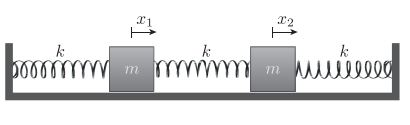
\includegraphics[width=0.6\textwidth]{Figures/A.JPG}
	\end{framed}
	\caption{Two blocks are attached to three springs \cite{Departme83:online}.}
	\label{fig:1}
\end{figure}

 \begin{figure}[hbt!]
	\centering
	\begin{framed}
	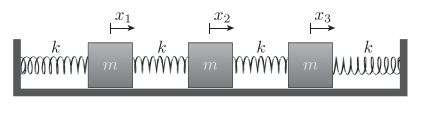
\includegraphics[width=0.6\textwidth]{Figures/E.JPG}
	\end{framed}
	\caption{Three blocks are attached to four springs \cite{Departme83:online}.}
	\label{fig:5}
\end{figure}

So far, we've only worked with masses attached to Hooke's law springs, which are, of course, highly idealised systems. More realistically, for macroscopic one dimensional mechanical motions here we concerned $CO_2$ molecules. As illustrated in Figure \ref{fig:4}, carbon dioxide is a linear molecule with the carbon atom (of mass m and coordinate x2) in the middle and the oxygen atoms (of mass M and coordinates x1 and x3) at the two ends. The behavior of the atoms at the scale of molecules is, of course, governed by quantum mechanics, and hence classical mechanics is merely a rough approximation to the true behaviour of the $CO_2$ molecule.

 \begin{figure}[hbt!]
	\centering
	\begin{framed}
	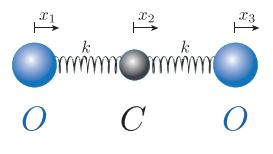
\includegraphics[width=0.35\textwidth]{Figures/D.JPG}
		\end{framed}
	\caption{The carbon dioxide molecule \cite{Departme83:online}.}
	\label{fig:4}
\end{figure}

\subsubsection{Coupled pendulums}

Two m-mass balls are tied to two equal-length $l$ strings to form side-by-side pendulums of equal period. As shown in Figure \ref{fig:2}, a weak spring $k$ is now coupled to the two balls. 

 \begin{figure}[hbt!]
	\centering
	\begin{framed}
	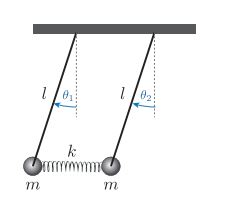
\includegraphics[width=0.38\textwidth]{Figures/B.JPG}
		\end{framed}
	\caption{Coupled pendulum \cite{Departme83:online}.}
	\label{fig:2}
\end{figure}

\subsubsection{ A planar system: masses in an equilateral triangle}

All particles and springs were aligned along a straight line and were only permitted to oscillate along that same straight line. Figure \ref{fig:3} depicts the normal-mode oscillations of a system with three equal masses $m$ and three equal springs $k$ in the shape of an equilateral triangle.

 \begin{figure}[hbt!]
	\centering
	\begin{framed}
	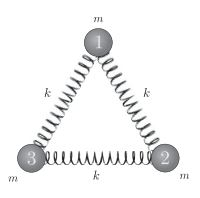
\includegraphics[width=0.33\textwidth]{Figures/C.JPG}
	\end{framed}
	\caption{Masses in an equilateral triangle
 \cite{Departme83:online}.}
	\label{fig:3}
\end{figure}

When a system is aroused into oscillations that are a mixture of normal modes \cite{cochelin20197th}, the motion will alter with time. Perhaps one of the masses will decrease amplitude and transfer energy to another mass, which will then return the energy \cite{kerschen2009nonlinear}. Even if the oscillations are all at the same frequency, such motion is totally distinguishable from simple harmonic motion and hence does not represent a normal mode. The transfer of energy usually occurs at a frequency that is significantly different from the frequency of oscillation.

\subsection{Degree of freedom}

\paragraph{}

Assume there are $N$ particles that can only move in one dimension. Then we define there seem to be N degrees of freedom (DOF) \cite{rosenberg1962normal}, $x_1, x_2,...x_N$, which are the positions observed along each particle's single dimension. If somehow the $N$ particles are instead permitted to travel in two dimensions, there are $2N$ degrees of freedom (DOF), $x_1, y_1,...x_N, y_N$, and so on. In case of that, Degrees of freedom (DOF) relate to the maximum number of logically independent values in a data sample, which are values with the freedom to fluctuate. DOF can be calculated using the below equation \eqref{1} and its corresponding constant values. 

\begin{equation}
    \label{1}
    DOF = (N \times n ) - k
\end{equation}

Where, \\
$n$ =  Number of dimensions \\
$N$ = Number of particles\\
$k$ = Number of constraints


\subsection{Euler-Lagrange equation}
\label{lag}

\paragraph{}

In this section, we'll learn about an entirely new way of seeing the world. Imagine the mass on the end of a spring. Of course, we can evaluate this by using $F = ma$ (Newton's second law) \cite{sharma2014isaac} to write out $m\Ddot{x} = k\Dot{x}$ \cite{zhong2019reliability}. As we all know, the solutions to such an equation are sinusoidal functions. However, we can sort things out by utilising a different strategy that does not reinforce F = ma. This new strategy is preferable to using Newton's second law in many (perhaps most) physical conditions. Here we now look at the lagrangian method. 

\begin{equation}
    \label{2}
    F_i = m\Ddot{x_i}
\end{equation}

The kinetic energy function, which is the time derivative of the momentum $p_1 = \partial T / \partial \Dot{x}$, determines the right side of this equation \eqref{2}. while the right hand side is a derivative of the potential energy, $- \partial U / \partial x_i$. . As $T$ is independent of $x_i$ and $U$ is independent of ˙$x_i$ in these coordinates, In terms of the Lagrangian, we can write both sides. 

\begin{equation}
    \label{3}
    L = T -U 
\end{equation}

Which is then a function of both the coordinates and their velocities. Thus we have established which will be known as Lagrange’s equation

\begin{equation}
    \label{4}
    \frac{d}{dt}(\frac{\partial L}{\partial \dot{xi}})-\frac{\partial L}{\partial xi} = 0 
\end{equation}

Here, $x = (x_1, . . . , x_N )$ and likewise $\dot{x}˙ = (\dot{x_1}, . . . , \dot{x_N})$. And also we can write \eqref{3} where
$T$ is the kinetic energy and $V$ is the potential energy. In the simplest cases, $T = T(\dot{x})$ and $V = V (x)$, The solution to a given mechanical problem is obtained by solving a set of $N$ second-order differential equations known as Euler-Lagrange equations of motion,

\begin{equation}
    \label{5}
    \frac{d}{dt}(\frac{\partial L}{\partial \dot{xi}})-\frac{\partial L}{\partial xi} = 0 
\end{equation}

\subsection{Numerical analysis}
\label{Num}

\paragraph{}
Numerical analysis is a branch of mathematics that teaches computer methods for studying and solving mathematical issues \cite{burden2015numerical}. In this section, we look at numerical approaches for solving the most frequent mathematical problems and analyse the errors that can occur while using these methods. Because practically all computation is now done on digital computers, we also explore the consequences for numerical method implementation.

The investigation of error is vital to numerical analysis. Most numerical approaches produce responses that are simply approximations to the intended genuine solution, and it is critical to understand the associated error and, if feasible, estimate or constrain it \cite{heydari2016theoretical}. This study looks at the numerous errors that can occur in a situation. The representation of numbers in computers, as well as the mistake in computer arithmetic, are investigated \cite{cui2018numerical}. The general results on the propagation of errors in calculations are presented, along with a detailed examination of errors in summing processes. Especially in this study, we will consider the Runge Kutta fourth-order (RK4) method \cite{islam2015accurate}. 

\subsubsection{Runge Kutta fourth order method}
\label{RK}
The fourth-order Runge-Kutta technique explains the lengthy computation of numerous unknowns, and the comprehensive step-by-step derivation and analysis can be found in many publications \cite{tan2012general} \cite{mehdi2017using}. Because of the method's importance in mathematics and applied science/engineering. By reviewing specific, possibly well-known papers, we simplify and minimise the complexity of their derivation and analysis by proposing a step-by-step derivation of the method.

In 1901, two German men, Carl Runge (1856-1927) and Martin Kutta (1867-1944), devised the Runge-Kutta Method \cite{tobies2012iris}. Carl Runge created numerical methods for solving the differential equations that evolved from his research on atomic spectra. These numerical techniques are still in use today. He employed so much mathematics in his studies that physicists mistook him for a mathematician, and he employed so much physics that mathematicians mistook him for a physicist. His name is now synonymous with the Runge-Kutta methods for numerically solving differential equations. Kutta, another German applied mathematician, is well recognised for his contribution to the Kutta-Joukowski theory of airfoil lift in aerodynamics, which is based on differential equations \cite{trefethen2015invented}. 

\newpage

\subsubsection{Runge-Kutta 4th order method to solve differential equation}

Given following inputs \cite{RungeKut7:online}. 

\begin{itemize}
    \item An ordinary differential equation that expresses the value of $dy/dt$ in terms of $t$ and $y$.
    \item Initial value of $y$, i.e., $y(0)$. 
\end{itemize}

\begin{equation}
    {{dy(t)} \over {dt}} = y'(t) = f(y(t),t), \quad \quad {\rm{with\;}} y(t_0)=y_0
\end{equation}

The evolution of the Fourth Order Runge-Kutta method closely parallels that of the second Order and will not be discussed in depth here. The fourth order method, like the second order method, has several variations that all employ four estimates to the slope. To determine the slope at some time t0 (assuming we just have an approximation to $y(t_0)$ (which we call $y^*(t_0)$), we will utilise the following slope approximations.

 \begin{figure}[hbt!]
	\centering
	\begin{framed}
	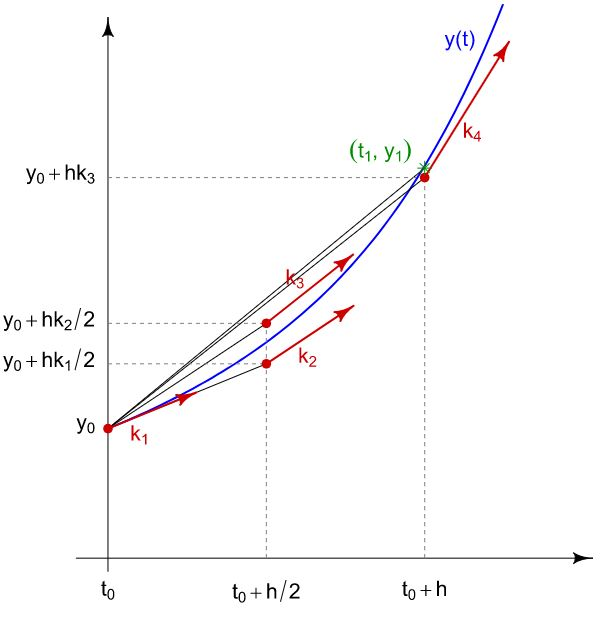
\includegraphics[width=0.6\textwidth]{Figures/F.JPG}
		\end{framed}
	\caption{Slopes used by the classical Runge-Kutta method \cite{hossain2017comparative}.}
	\label{fig:6}
\end{figure}

\newpage

\begin{equation}
    {k_1} = f({y^*}({t_0}),{t_0})
\end{equation}

\begin{equation}
    {k_2} = f\left( {{y^*}({t_0}) + {k_1}{h \over 2},{t_0} + {h \over 2}} \right)
\end{equation}

\begin{equation}
     {k_3} = f\left( {{y^*}({t_0}) + {k_2}{h \over 2},{t_0} + {h \over 2}} \right) 
\end{equation}

\begin{equation}
    {k_4} = f\left( {{y^*}({t_0}) + {k_3}h,{t_0} + h} \right)
\end{equation}

Each one of these slope estimates can be directly explained \cite{FourthOr20:online}.

\begin{itemize}
    \item $k_1$ is the slope at the beginning of the time step (this is the same as $k_1$ in the first and second order methods).
    
\item If we use the slope $k_1$ to step halfway through the time step, then $k_2$ is an estimate of the slope at the midpoint. This is the same as the slope$_2$, from the second order midpoint method. This slope proved to be more accurate than $k_1$ for making new approximations for y(t).

\item If we use the slope $k_2$ to step halfway through the time step, then $k_3$ is another estimate of the slope at the midpoint.

\item Finally, we use the slope, $k_3$, to step all the way across the time step$(t_0, t_0+h)$, and $k_4$ is an estimate of the slope at the endpoint. 
\end{itemize}

We then use a weighted sum of these slopes to get our final estimate of $y^*(t_0+h)$.

\begin{equation}
    {y^*}({t_0} + h) = {y^*}({t_0}) + {{{k_1} + 2{k_2} + 2{k_3} + {k_4}} \over 6}h 
\end{equation}



\begin{equation}
   {y^*}({t_0} + h) = {y^*}({t_0}) + \left( {{1 \over 6}{k_1} + {1 \over 3}{k_2} + {1 \over 3}{k_3} + {1 \over 6}{k_4}} \right)h
\end{equation}

\begin{equation}
   {y^*}({t_0} + h) =  {y^*}({t_0}) + mh
\end{equation}

 {\rm{where\;}}m{\rm{\;is\;a\;weighted\;average\; slope\; approximation.}}

The approach is comparable to the second order endpoint method \cite{dontchev2000second}, which employed an equal weighting of the slopes at the start and end of the interval. The weighting of the midpoint slopes ($k_2$ and $k_3$) is larger than that of the endpoint slopes ($k_1$ and $k_4$) in this case, because we expect these to be a better estimate of the slope while travelling from $y^*(t_0)$ to $y^*(t_0+h)$.


\newpage
\section{Problem statement and objectives}
\paragraph{}
Vibration analysis for frequency response and temporal response has become essential for significant industrial machines and other troubleshooting applications. The computation of natural frequencies for a finite coupled freedom system (one dimension and two dimension)  n-degree freedom system (one dimension and two dimension) and comparative amplitudes of vibrating masses assists the designer in selecting system parameters and allow the implementation for safer operations. As we all know, classical mathematical approaches are insufficient for real-time frequency response processing because they require more time and effort. We sought to examine a few freedom system for natural frequencies and hence pure mode forms in this study. The pure mode patterns can then be placed to obtain the system's real displacement pattern. We created below coupled freedom system by writing a software in the MatLab platform. The project objectives proposed for this study are expected to contribute to the current level of knowledge regarding the dynamic behaviour of coupled spring-mass systems compared to numerical solutions. The objectives
are listed below.

\begin{enumerate}
    \item Investigate the motion for undamped linear systems with  coupled two degrees of freedom.
    \item Investigate the motion for undamped linear systems with coupled many degrees of freedom. 
    \item Investigate the two-dimensional spring motion: the mass
m is free to move in the $XY$ plane. 
\end{enumerate}




\section{Project structure}
\paragraph{}

In the chapter one, introduction into the project and other background of study will be discussed. This chapter is presented coupled oscillations, degree of freedom, Lagrangian and numerical methods. In this chapter problem scope of the project and objectives will be discussed as well.  When it comes to the chapter two, there will be discussed the process and concepts corresponding to the methodology. Behalf of the methodology, above mentioned objectives will be explained under each and each sections. Both 1D and 2D spring mass models are considered their behaviour, assumptions and behind scene of the physics background. This will be demonstrated the both physics and mathematical concepts to explain the given objectives.  After that, in the chapter three,  the before obtaining the results theoretically  all obtained differential equations will be solved and explained by numerical method of Runge kutta fourth order. In chapter four, all the results of spring mass models will be discussed. Finally, chapter six brings the conclusion of the whole project.   
\paragraph{}







































%\chapter{Introduction}
\label{chap:01}


\paragraph{}
The vibration phenomenon can be observed in various standard settings, including speaking, vision, auditioning, and other activities involving human interaction owing to mechanical waves and digital communication via electromagnetic waves \cite{tse1963mechanical}. Also, Vibrations are a part of our everyday lives, and individuals encounter them in various ways. This phenomenon is required in various engineering applications, such as car suspension, where vibration increases driver comfort. They range from small-scale motions of atoms in substances to large-scale swaying of buildings and other structures and can be welcomed and intended, or bothersome and, in the worst case, harmful \cite{mori2017mechanical}. Oscillatory motion is joint, and physicists frequently idealise these examples of vibration into instances of a beneficial fiction, the harmonic oscillator. 

A mathematical depiction of a physical, biological, or information system is a simulation \cite{wada1972equivalent}. Models enable us to think about a system and forecast its behaviour. A dynamical system is one in which the consequences of actions do not arise instantly. For example, a headache does not go away immediately after taking aspirin; it takes time to take action. Additional funding for a development project does not enhance profits in the short term, but it may do the same in the longer - term in enterprise applications. All of these are instances of dynamical systems, in which the system's behaviour varies through time. As previously stated, the mass-spring model has been widely utilised to simulate deformable objects for facial animation \cite{keeve1998deformable}, animation of artificial animals \cite{tu1994artificial}, cloth draping \cite{ji2006three}, garment animation \cite{provot1995deformation}, and, more recently, surgical simulations \cite{sorensen2007virtual}. Recent enhancements to this model include the inverse dynamics approach to eliminate super elongation of the springs \cite{mozafary2016study} and the implicit integration method to take substantial time steps. 


The mass-spring model can be considered a discrete approximation method for solving the Lagrange partial differential equation of motion \cite{baleanu2020new}. Because of the extreme discretisation, the mass-spring model will only approximate the continuous object in some ways. The mass-spring model and the finite element method (FEM) \cite{duan2014volume} were compared, and it was determined that an exact simulation using the mass-spring model is unattainable. This project could clarify why there hasn't been much research on optimising the parameters of the mass-spring model. Even though the mass-spring model cannot provide an exact simulation, certain reasonable parameter sets provide more physically realistic simulations than others. The mass-spring model is currently implemented using a trial-and-error approach to determine parameter values for many applications. Aside from the fact that the criteria are highly subjective, the process is extremely laborious and time-consuming.

The capacity to forecast and reduce structural vibrations has recently attracted more attention. Vibrations originate from either external sources, such as wind, or internal sources, including friction between mechanical pieces of a system. The most typical scenario of vibration is break squeal in automobiles \cite{suggs1969application}. As a result, researchers have focused their efforts on studying vibration phenomena and their applicability in real life \cite{levitan1960forced} \cite{pellicer2004analysis} \cite{grandmont2006viscoelastic}. Because their occurrence is inherently dependent on the unique internal properties, the motion can be described mathematically as the unstable homogeneous solution to the homogeneous equations of motion. Furthermore, mathematical solutions will be discussed in detail in future chapters. 

\section{Background of the study}
\label{sec:1.1}

\paragraph{}

The study of linked oscillators has since become an important branch of mathematics, with applications in physics, biology, and chemistry \cite{Chapter427:online}. Coupled oscillators are seen in biological systems as well \cite{winfree1967biological} \cite{hannay2018macroscopic}. Most species directly correspond to numerous patterns in our environment, such as the earth's rotation around the sun, the alternation of night and day, or the tides. Organisms demonstrate periodicities due to their environment and exhibit innate periodic activity. Inhalation, blood circulation, chewing, molecular motion and galloping are all instances of rhythmic motion patterns. Waves are the propagation of oscillations in space caused by the connection of individual oscillators. A straightforward exercise is to strike the right piano note, which sounds the tuning-fork tuned to the same frequency as the key we hit. Another scenario is the powerful sound of the frequency corresponding to the resonance frequency of the glass breaking a delicate wine glass. In this section coupled oscillators, Degree of freedom, Euler's Lagrange, Runge kutta method (fourth order) and other relevant background will be discussed. 


\subsection{Coupled oscillators}

\paragraph{}

Like the small-amplitude swinging of a pendulum, some oscillations are extremely simple and can be approximated by a single mass on the end of a Hooke'slaw spring. And some are more complex but could still be represented by two or more masses and two or more springs. Examples are compound mechanical systems, oscillating electrical circuits with multiple branches, multi-atom molecules, and elastic materials.  Here we display the few example of coupled oscillators used to understand oscillations like these.

\subsubsection{Linear systems of masses and springs}
As shown in Figure \ref{fig:1}, the blocks are attached to three springs, and the outer springs are likewise attached to stationary walls. The outer springs each have a force constant $k$, while the inner spring has a force constant $k'$. When the blocks are at rest, the springs are untethered. Let $x_1$ and $x_2$ represent the displacements of blocks 1 and 2 from their equilibrium locations, positive to the right. Assume three blocks are connected to four springs: In the equilibrium position, the springs are again unstretched, and the blocks can only move horizontally. Each outer spring's far end is linked to a stationary wall. The three blocks' displacements from equilibrium are $x_1$,$x_2$, and $x_3$, all positive to the right. Assume the blocks have the same mass $m$ and the same force constant $k$, as shown in Figure \ref{fig:5}.


 \begin{figure}[hbt!]
	\centering
	\begin{framed}
	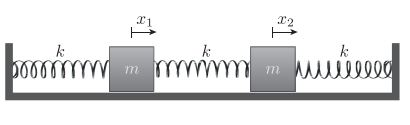
\includegraphics[width=0.6\textwidth]{Figures/A.JPG}
	\end{framed}
	\caption{Two blocks are attached to three springs \cite{Departme83:online}.}
	\label{fig:1}
\end{figure}

 \begin{figure}[hbt!]
	\centering
	\begin{framed}
	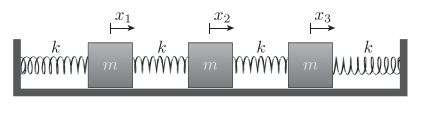
\includegraphics[width=0.6\textwidth]{Figures/E.JPG}
	\end{framed}
	\caption{Three blocks are attached to four springs \cite{Departme83:online}.}
	\label{fig:5}
\end{figure}

So far, we've only worked with masses attached to Hooke's law springs, which are, of course, highly idealised systems. More realistically, for macroscopic one dimensional mechanical motions here we concerned $CO_2$ molecules. As illustrated in Figure \ref{fig:4}, carbon dioxide is a linear molecule with the carbon atom (of mass m and coordinate x2) in the middle and the oxygen atoms (of mass M and coordinates x1 and x3) at the two ends. The behavior of the atoms at the scale of molecules is, of course, governed by quantum mechanics, and hence classical mechanics is merely a rough approximation to the true behaviour of the $CO_2$ molecule.

 \begin{figure}[hbt!]
	\centering
	\begin{framed}
	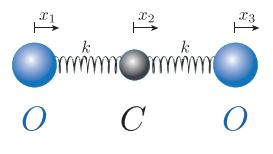
\includegraphics[width=0.35\textwidth]{Figures/D.JPG}
		\end{framed}
	\caption{The carbon dioxide molecule \cite{Departme83:online}.}
	\label{fig:4}
\end{figure}

\subsubsection{Coupled pendulums}

Two m-mass balls are tied to two equal-length $l$ strings to form side-by-side pendulums of equal period. As shown in Figure \ref{fig:2}, a weak spring $k$ is now coupled to the two balls. 

 \begin{figure}[hbt!]
	\centering
	\begin{framed}
	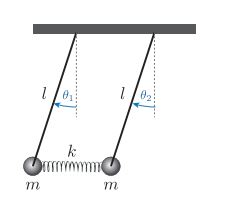
\includegraphics[width=0.38\textwidth]{Figures/B.JPG}
		\end{framed}
	\caption{Coupled pendulum \cite{Departme83:online}.}
	\label{fig:2}
\end{figure}

\subsubsection{ A planar system: masses in an equilateral triangle}

All particles and springs were aligned along a straight line and were only permitted to oscillate along that same straight line. Figure \ref{fig:3} depicts the normal-mode oscillations of a system with three equal masses $m$ and three equal springs $k$ in the shape of an equilateral triangle.

 \begin{figure}[hbt!]
	\centering
	\begin{framed}
	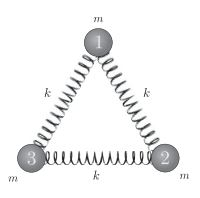
\includegraphics[width=0.33\textwidth]{Figures/C.JPG}
	\end{framed}
	\caption{Masses in an equilateral triangle
 \cite{Departme83:online}.}
	\label{fig:3}
\end{figure}

When a system is aroused into oscillations that are a mixture of normal modes \cite{cochelin20197th}, the motion will alter with time. Perhaps one of the masses will decrease amplitude and transfer energy to another mass, which will then return the energy \cite{kerschen2009nonlinear}. Even if the oscillations are all at the same frequency, such motion is totally distinguishable from simple harmonic motion and hence does not represent a normal mode. The transfer of energy usually occurs at a frequency that is significantly different from the frequency of oscillation.

\subsection{Degree of freedom}

\paragraph{}

Assume there are $N$ particles that can only move in one dimension. Then we define there seem to be N degrees of freedom (DOF) \cite{rosenberg1962normal}, $x_1, x_2,...x_N$, which are the positions observed along each particle's single dimension. If somehow the $N$ particles are instead permitted to travel in two dimensions, there are $2N$ degrees of freedom (DOF), $x_1, y_1,...x_N, y_N$, and so on. In case of that, Degrees of freedom (DOF) relate to the maximum number of logically independent values in a data sample, which are values with the freedom to fluctuate. DOF can be calculated using the below equation \eqref{1} and its corresponding constant values. 

\begin{equation}
    \label{1}
    DOF = (N \times n ) - k
\end{equation}

Where, \\
$n$ =  Number of dimensions \\
$N$ = Number of particles\\
$k$ = Number of constraints


\subsection{Euler-Lagrange equation}
\label{lag}

\paragraph{}

In this section, we'll learn about an entirely new way of seeing the world. Imagine the mass on the end of a spring. Of course, we can evaluate this by using $F = ma$ (Newton's second law) \cite{sharma2014isaac} to write out $m\Ddot{x} = k\Dot{x}$ \cite{zhong2019reliability}. As we all know, the solutions to such an equation are sinusoidal functions. However, we can sort things out by utilising a different strategy that does not reinforce F = ma. This new strategy is preferable to using Newton's second law in many (perhaps most) physical conditions. Here we now look at the lagrangian method. 

\begin{equation}
    \label{2}
    F_i = m\Ddot{x_i}
\end{equation}

The kinetic energy function, which is the time derivative of the momentum $p_1 = \partial T / \partial \Dot{x}$, determines the right side of this equation \eqref{2}. while the right hand side is a derivative of the potential energy, $- \partial U / \partial x_i$. . As $T$ is independent of $x_i$ and $U$ is independent of ˙$x_i$ in these coordinates, In terms of the Lagrangian, we can write both sides. 

\begin{equation}
    \label{3}
    L = T -U 
\end{equation}

Which is then a function of both the coordinates and their velocities. Thus we have established which will be known as Lagrange’s equation

\begin{equation}
    \label{4}
    \frac{d}{dt}(\frac{\partial L}{\partial \dot{xi}})-\frac{\partial L}{\partial xi} = 0 
\end{equation}

Here, $x = (x_1, . . . , x_N )$ and likewise $\dot{x}˙ = (\dot{x_1}, . . . , \dot{x_N})$. And also we can write \eqref{3} where
$T$ is the kinetic energy and $V$ is the potential energy. In the simplest cases, $T = T(\dot{x})$ and $V = V (x)$, The solution to a given mechanical problem is obtained by solving a set of $N$ second-order differential equations known as Euler-Lagrange equations of motion,

\begin{equation}
    \label{5}
    \frac{d}{dt}(\frac{\partial L}{\partial \dot{xi}})-\frac{\partial L}{\partial xi} = 0 
\end{equation}

\subsection{Numerical analysis}
\label{Num}

\paragraph{}
Numerical analysis is a branch of mathematics that teaches computer methods for studying and solving mathematical issues \cite{burden2015numerical}. In this section, we look at numerical approaches for solving the most frequent mathematical problems and analyse the errors that can occur while using these methods. Because practically all computation is now done on digital computers, we also explore the consequences for numerical method implementation.

The investigation of error is vital to numerical analysis. Most numerical approaches produce responses that are simply approximations to the intended genuine solution, and it is critical to understand the associated error and, if feasible, estimate or constrain it \cite{heydari2016theoretical}. This study looks at the numerous errors that can occur in a situation. The representation of numbers in computers, as well as the mistake in computer arithmetic, are investigated \cite{cui2018numerical}. The general results on the propagation of errors in calculations are presented, along with a detailed examination of errors in summing processes. Especially in this study, we will consider the Runge Kutta fourth-order (RK4) method \cite{islam2015accurate}. 

\subsubsection{Runge Kutta fourth order method}
\label{RK}
The fourth-order Runge-Kutta technique explains the lengthy computation of numerous unknowns, and the comprehensive step-by-step derivation and analysis can be found in many publications \cite{tan2012general} \cite{mehdi2017using}. Because of the method's importance in mathematics and applied science/engineering. By reviewing specific, possibly well-known papers, we simplify and minimise the complexity of their derivation and analysis by proposing a step-by-step derivation of the method.

In 1901, two German men, Carl Runge (1856-1927) and Martin Kutta (1867-1944), devised the Runge-Kutta Method \cite{tobies2012iris}. Carl Runge created numerical methods for solving the differential equations that evolved from his research on atomic spectra. These numerical techniques are still in use today. He employed so much mathematics in his studies that physicists mistook him for a mathematician, and he employed so much physics that mathematicians mistook him for a physicist. His name is now synonymous with the Runge-Kutta methods for numerically solving differential equations. Kutta, another German applied mathematician, is well recognised for his contribution to the Kutta-Joukowski theory of airfoil lift in aerodynamics, which is based on differential equations \cite{trefethen2015invented}. 

\newpage

\subsubsection{Runge-Kutta 4th order method to solve differential equation}

Given following inputs \cite{RungeKut7:online}. 

\begin{itemize}
    \item An ordinary differential equation that expresses the value of $dy/dt$ in terms of $t$ and $y$.
    \item Initial value of $y$, i.e., $y(0)$. 
\end{itemize}

\begin{equation}
    {{dy(t)} \over {dt}} = y'(t) = f(y(t),t), \quad \quad {\rm{with\;}} y(t_0)=y_0
\end{equation}

The evolution of the Fourth Order Runge-Kutta method closely parallels that of the second Order and will not be discussed in depth here. The fourth order method, like the second order method, has several variations that all employ four estimates to the slope. To determine the slope at some time t0 (assuming we just have an approximation to $y(t_0)$ (which we call $y^*(t_0)$), we will utilise the following slope approximations.

 \begin{figure}[hbt!]
	\centering
	\begin{framed}
	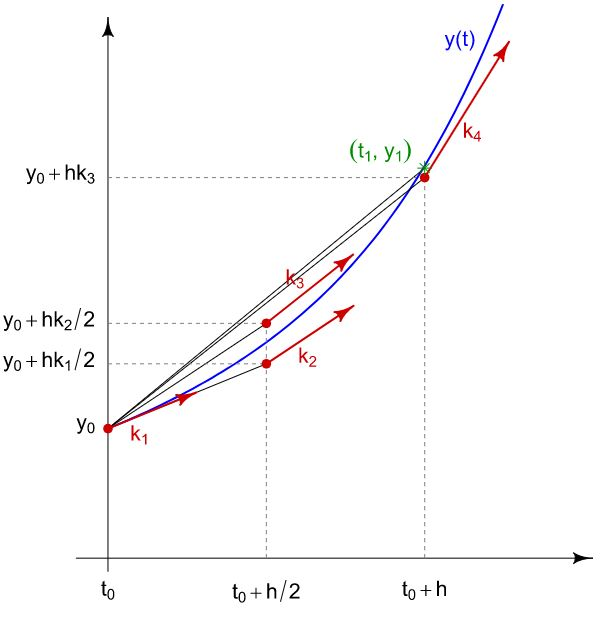
\includegraphics[width=0.6\textwidth]{Figures/F.JPG}
		\end{framed}
	\caption{Slopes used by the classical Runge-Kutta method \cite{hossain2017comparative}.}
	\label{fig:6}
\end{figure}

\newpage

\begin{equation}
    {k_1} = f({y^*}({t_0}),{t_0})
\end{equation}

\begin{equation}
    {k_2} = f\left( {{y^*}({t_0}) + {k_1}{h \over 2},{t_0} + {h \over 2}} \right)
\end{equation}

\begin{equation}
     {k_3} = f\left( {{y^*}({t_0}) + {k_2}{h \over 2},{t_0} + {h \over 2}} \right) 
\end{equation}

\begin{equation}
    {k_4} = f\left( {{y^*}({t_0}) + {k_3}h,{t_0} + h} \right)
\end{equation}

Each one of these slope estimates can be directly explained \cite{FourthOr20:online}.

\begin{itemize}
    \item $k_1$ is the slope at the beginning of the time step (this is the same as $k_1$ in the first and second order methods).
    
\item If we use the slope $k_1$ to step halfway through the time step, then $k_2$ is an estimate of the slope at the midpoint. This is the same as the slope$_2$, from the second order midpoint method. This slope proved to be more accurate than $k_1$ for making new approximations for y(t).

\item If we use the slope $k_2$ to step halfway through the time step, then $k_3$ is another estimate of the slope at the midpoint.

\item Finally, we use the slope, $k_3$, to step all the way across the time step$(t_0, t_0+h)$, and $k_4$ is an estimate of the slope at the endpoint. 
\end{itemize}

We then use a weighted sum of these slopes to get our final estimate of $y^*(t_0+h)$.

\begin{equation}
    {y^*}({t_0} + h) = {y^*}({t_0}) + {{{k_1} + 2{k_2} + 2{k_3} + {k_4}} \over 6}h 
\end{equation}



\begin{equation}
   {y^*}({t_0} + h) = {y^*}({t_0}) + \left( {{1 \over 6}{k_1} + {1 \over 3}{k_2} + {1 \over 3}{k_3} + {1 \over 6}{k_4}} \right)h
\end{equation}

\begin{equation}
   {y^*}({t_0} + h) =  {y^*}({t_0}) + mh
\end{equation}

 {\rm{where\;}}m{\rm{\;is\;a\;weighted\;average\; slope\; approximation.}}

The approach is comparable to the second order endpoint method \cite{dontchev2000second}, which employed an equal weighting of the slopes at the start and end of the interval. The weighting of the midpoint slopes ($k_2$ and $k_3$) is larger than that of the endpoint slopes ($k_1$ and $k_4$) in this case, because we expect these to be a better estimate of the slope while travelling from $y^*(t_0)$ to $y^*(t_0+h)$.


\newpage
\section{Problem statement and objectives}
\paragraph{}
Vibration analysis for frequency response and temporal response has become essential for significant industrial machines and other troubleshooting applications. The computation of natural frequencies for a finite coupled freedom system (one dimension and two dimension)  n-degree freedom system (one dimension and two dimension) and comparative amplitudes of vibrating masses assists the designer in selecting system parameters and allow the implementation for safer operations. As we all know, classical mathematical approaches are insufficient for real-time frequency response processing because they require more time and effort. We sought to examine a few freedom system for natural frequencies and hence pure mode forms in this study. The pure mode patterns can then be placed to obtain the system's real displacement pattern. We created below coupled freedom system by writing a software in the MatLab platform. The project objectives proposed for this study are expected to contribute to the current level of knowledge regarding the dynamic behaviour of coupled spring-mass systems compared to numerical solutions. The objectives
are listed below.

\begin{enumerate}
    \item Investigate the motion for undamped linear systems with  coupled two degrees of freedom.
    \item Investigate the motion for undamped linear systems with coupled many degrees of freedom. 
    \item Investigate the two-dimensional spring motion: the mass
m is free to move in the $XY$ plane. 
\end{enumerate}




\section{Project structure}
\paragraph{}

In the chapter one, introduction into the project and other background of study will be discussed. This chapter is presented coupled oscillations, degree of freedom, Lagrangian and numerical methods. In this chapter problem scope of the project and objectives will be discussed as well.  When it comes to the chapter two, there will be discussed the process and concepts corresponding to the methodology. Behalf of the methodology, above mentioned objectives will be explained under each and each sections. Both 1D and 2D spring mass models are considered their behaviour, assumptions and behind scene of the physics background. This will be demonstrated the both physics and mathematical concepts to explain the given objectives.  After that, in the chapter three,  the before obtaining the results theoretically  all obtained differential equations will be solved and explained by numerical method of Runge kutta fourth order. In chapter four, all the results of spring mass models will be discussed. Finally, chapter six brings the conclusion of the whole project.   
\paragraph{}







































%\input{ch2.tex}
%\include{ch2.tex}
\chapter{Methodology}
\label{chap:03}
\paragraph{}

Several ideas must be known in order to determine dynamic vibration analysis. There are several elements that impact which model is applied and understood. To determine which model to utilise, the complexity of the system and the number of influencing parameters must be determined. This chapter will go over the different coupled spring mass systems oscillations vibration involving many objects (usually without damping or driving) and how they behave with different parameter values, as well as complex analysis using the Runge Kutta fourth order method (section \ref{RK}) and how to obtain the numerical analysis using software MATLAB. Roughly working, the count of the degree of freedom goes as follows: two and $n^{th}$ for linear systems. To obtain vibration of the two dimensional (2D) spring mass system, which has  one mass and  $n^{th}$ mass respectively. 




\section{Investigate the motion for undamped linear spring mass system with  coupled two degrees of freedom}
\label{2DOF}

The simple one degree of freedom (1DOF) \cite{tsai2020design} systems examined in the preceding section are pretty helpful in developing an understanding of the general properties of vibrating systems. They are far too simplistic to approximate the majority of real-world systems. Real systems have multiple degrees of freedom. Real-world systems are almost never linear. It turns out that they are, but you will not be convinced unless you know how to evaluate more genuine issues and notice how they frequently behave just like the simple idealizations. As early stated in this section spring system of two degrees of freedom (2DOF) \cite{eiss1964vibration} will be discussed with details. 

\subsection{Equations of motion for undamped linear spring mass system with 2DOF }

\paragraph{}
Newton’s second law of motion tells us how a point mass moves in response to a force. But as early stated in this project we use only Lagrange equation (section \ref{lag}) to obtain the equations of motion given coupled systems. In this section, we are given two masses, each of mass $m_1$ and $m_2$, sitting on a frictionless horizontal surface.  The blocks are attached to three springs, and the outer springs are also attached to stationary walls, as shown in figure \ref{fig:7}. The two outer springs each have force constant $k_1$ and $k_3$ respectively, and the inner spring has force constant $k_2$. When the blocks are at rest the springs are unstretched.

Let $_1$ and $x_2$ represent the displacements of mass 1 and 2 from their equilibrium locations, positive to the right. Our goal is to determine the differential equations of motion for each mass and then solve them to determine $x_1(t)$ and $x_2 (t)$. In given figure \ref{fig:6} Degree of freedom (DOF) = 3$\times$2-4 =2 from equation \eqref{1}. Therefore we can say in the figure \ref{fig:6} has two body degree of freedom.



 \begin{figure}[hbt!]
	\centering
	\begin{framed}
	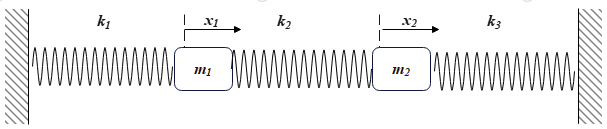
\includegraphics[width=0.7\textwidth]{Figures/G.png}
		\end{framed}
	\caption{ Undamped linear spring mass systems with 2DOF.}
	\label{fig:7}
\end{figure}

In the section, given figure \ref{fig:6} is a two degree of freedom system (2DOF), governed by two differential equations. The governing equations can also be achieved by following Lagrange's Equation directly. The expression for kinetic energy is,

\begin{equation}
    T = \frac{1}{2}m_1\dot{x_1}^2 + \frac{1}{2}m_2\dot{x_2}^2
\end{equation}
And also, the expression for potential energy is,
\begin{equation}
    V = \frac{1}{2}k_1x^2+\frac{1}{2}k_2(x_2-x_1)^2+\frac{1}{2}k_3x_3^2
\end{equation}

 Consider the following seemingly silly combination of the kinetic and potential energies ($T$ and $V$ , respectively), It is denoted by $L$,
\begin{equation}
\label{aaa}
    L = T-V
\end{equation}


Applying Lagrange’s equation to equation \eqref{aaa},
\begin{equation}
    \frac{d}{dt}(\frac{\partial L}{\partial \dot{x1}})-\frac{\partial L}{\partial x1} = 0 
\end{equation}
\begin{equation}
     \frac{d}{dt}(\frac{\partial L}{\partial \dot{x2}})-\frac{\partial L}{\partial x2} = 0
\end{equation}

Governing differential equations \cite{cartwright1945non} are based on balance laws for mass and momentum, and completed by constitutive relations for the fluid and solid phases as well as their mutual interactions. In the section  equation \eqref{aaa} its results we can obtain the governing equations as,

\newpage

\begin{equation}
\label{aab}
    m_1\dot{x_1}+(k_1+k_2)x_1-k_2x_2=0
\end{equation}
\begin{equation}
\label{aac}
    m_2\dot{x_2}-k_2x_1+(k_2+k_3)x_2 = 0
\end{equation}

Clearly,  we were able to realised for multi degree of freedom systems, this approach (Lagrangian) has advantages over the force balancing approach using Newton’s law.

\subsection{Matrix form of equations of motion}

\paragraph{}

To approach vibration problems, we always put the equations of motion (\eqref{aab} and \eqref{aac}) in matrix form. The matrix form of the system of governing equations of motion is as follows and the component matrices are commonly named as listed below. 
\begin{equation}
    M \frac{d\dot{x^2}}{dt}+ Kx = 0
\end{equation}

\begin{equation}
\label{aad}
    [M]{\dot{X}}+[K]{X} = 0
\end{equation}

\begin{gather}
 \begin{bmatrix} m_1 & 0 \\ 0 & m_2 \end{bmatrix} \frac{d^2}{dt^2} \begin{bmatrix}
  x_1 \\ x_2
 \end{bmatrix} + \begin{bmatrix}
  k_1+k_2 & -k_2 \\ -k_2 & k_2+k_3
 \end{bmatrix}
 \begin{bmatrix}
  x_1 \\ x_2
 \end{bmatrix}
 =
  \begin{bmatrix}
0 \\0
   \end{bmatrix}
\end{gather}

\begin{gather}
    \begin{bmatrix}
m_1 & 0\\0& m_2 
\end{bmatrix}{\dot{X}} +
\begin{bmatrix}
k_1+k_2 &-k_2\\-k_2&k_2+k_3
\end{bmatrix}{X} = 0
\end{gather}


Where $x$ is a vector of the variables describing the motion,  $M$ is called the ‘mass matrix’ and $K$ is called the ‘Stiffness matrix’ for the system. $M$ and $K$ are 2$\times$2 matrices for a system with two masses (or, more broadly, two degrees of freedom). They are $n \times n$ matrices for a system with $n$ degrees of freedom.

\subsection{Natural frequencies and mode shapes for 2-degrees-of-freedom undamped linear system}
\paragraph{}

First. now let us go over the definitions of natural frequencies and mode shapes first. Remember that we may make a system vibrate by slightly pushing it from its static equilibrium state and then releasing it. The resulting motion will not be harmonic in general. Certain special initial displacements, on the other hand, will result in harmonic vibrations. These unique initial deflections are known as mode shapes, and the accompanying vibrational frequencies are known as natural frequencies \cite{kuether2014numerical} \cite{gigerenzer2011natural}. A vibrating system's natural frequencies are its most essential attribute. It is useful to have a straightforward method for calculating them.

To continue, we need to make the crucial assumption that the system has specific motions in which both masses oscillate at the same frequency. We will observe that for one-dimensional chains, there seem to be exactly as many normal modes as there are masses in the system. Each and every normal mode corresponds to a single frequency of motion, but the frequencies of normal modes can be vary. We may represent the general motion of any mass in terms of a superposition of normal modes once we have identified the movements associated with the normal modes and determined the normal mode frequencies. Assume that both masses move at the same frequency to find the normal mode frequencies.

\begin{equation}
\label{x1}
    x_1 = A_1e^{i\omega t}
\end{equation}

\begin{equation}
\label{x2}
    x_2 = A_2e^{i\omega t}
\end{equation}

Consider the double derivation of equation \eqref{x1} and \eqref{x2},

\begin{equation}
\label{x1}
    \Ddot{x_1}  = - \omega^2 A_1e^{i\omega t} = -\omega^2 x_1
\end{equation}

\begin{equation}
\label{x2}
   \Ddot{x_2}  = - \omega^2 A_2e^{i\omega t} = -\omega^2 x_2
\end{equation}
 
Where $A_1$ and $A_2$ are arbitrary constants.
 
Substituting these into the equations of motion \eqref{aab} and \eqref{aac}  gives us,

\begin{equation}
\label{x3}
    -\omega^2 m_1 A_1e^{i\omega t} +(k_1 + k_2) A_1e^{i\omega t}- k_2A_2e^{i\omega t}= 0
\end{equation}

\begin{equation}
    \label{x4}
    -\omega^2 m_2 A_2e^{i\omega t} - k_2 A_1 e^{i\omega t} + (k_2 + k_3)A_2e^{i\omega t} = 0 
\end{equation}

From equation \eqref{x3} and \eqref{x4}, since the exponential factor is common to all terms, we omit it and simplify, 

\begin{equation}
\label{x5}
    (\omega^2 m_1  -(k_1 + k_2)) A_1e^{i\omega t}+ k_2A_2e^{i\omega t}= 0
\end{equation}

\begin{equation}
    \label{x6}
   k_2 A_1 e^{i\omega t}  +(\omega^2 m_2  - (k_2 + k_3))A_2e^{i\omega t} = 0 
\end{equation}

And in matrix representation,

\begin{gather}
    \begin{bmatrix}
(\omega^2 m_1  -(k_1 + k_2)) & k_2\\k_2& (\omega^2 m_2  - (k_2 + k_3))
\end{bmatrix}\begin{bmatrix}
A_1 \\ A_2
\end{bmatrix}
 = 0
\end{gather}


For arbitrary frequencies the only solution of the equation is the “trivial” solution $A_1 = A_2 = 0$,  where both blocks remain at rest at their equilibrium positions. But from linear algebra we know that with just the right choice(s) of $\omega$ there are also non-trivial solution(s) if and only if the determinant of the coefficients vanishes, i.e., if and only if, 

\begin{gather}
    \begin{vmatrix}
(\omega^2 m_1  -(k_1 + k_2)) & k_2 \\
k_2 & (\omega^2 m_2  - (k_2 + k_3))
\end{vmatrix} = 0
\end{gather}

\begin{equation}
   \left( {{\omega ^2} - \frac{{{k_1} + {k_2}}}{{{m_1}}}} \right) \left( {{\omega ^2} - \frac{{{k_2} + {k_3}}}{{{m_2}}}} \right) - \frac{{k_2^2}}{{{m_1}{m_2}}} = 0
\end{equation}

\begin{equation}
    {\omega ^4} - \frac{{{k_1} + {k_2}}}{{{m_1}}}{\omega ^2} - \frac{{{k_2} + {k_3}}}{{{m_2}}}{\omega ^2}
+ \frac{{\left( {{k_1} + {k_2}} \right)\left( {{k_2} + {k_3}} \right)}}{{{m_1}{m_2}}} - \frac{{k_2^2}}{{{m_1}{m_2}}} = 0
\end{equation}

\begin{equation}
    {\omega ^4} - \left( {\frac{{{k_1} + {k_2}}}{{{m_1}}} + \frac{{{k_2} + {k_3}}}{{{m_2}}}} \right){\omega ^2}
+ \frac{{\left( {{k_1} + {k_2}} \right)\left( {{k_2} + {k_3}} \right)}}{{{m_1}{m_2}}} - \frac{{k_2^2}}{{{m_1}{m_2}}} = 0
\end{equation}

Finding solution this biquadratic equation, we find the eigen frequencies. Let us first obtain the discriminant. 

\begin{equation}
    D = {\left( {\frac{{{k_1} + {k_2}}}{{{m_1}}} + \frac{{{k_2} + {k_3}}}{{{m_2}}}} \right)^2}
- 4\left[ {\frac{{\left( {{k_1} + {k_2}} \right)\left( {{k_2} + {k_3}} \right)}}{{{m_1}{m_2}}} - \frac{{k_2^2}}{{{m_1}{m_2}}}} \right]
\end{equation}

\begin{equation}
    D ={\left( {\frac{{{k_1} + {k_2}}}{{{m_1}}}} \right)^2} + {\left( {\frac{{{k_2} + {k_3}}}{{{m_2}}}} \right)^2}
+ \frac{{2\left( {{k_1} + {k_2}} \right)\left( {{k_2} + {k_3}} \right)}}{{{m_1}{m_2}}}
- \frac{{4\left( {{k_1} + {k_2}} \right)\left( {{k_2} + {k_3}} \right)}}{{{m_1}{m_2}}}
+ \frac{{4k_2^2}}{{{m_1}{m_2}}}
\end{equation}

\begin{equation}
    D = {\left( {\frac{{{k_1} + {k_2}}}{{{m_1}}} - \frac{{{k_2} + {k_3}}}{{{m_2}}}} \right)^2}
+ \frac{{4k_2^2}}{{{m_1}{m_2}}}
\end{equation}

The formula will then explain the square of the eigen frequencies.

\begin{equation}
    {\omega ^2} = \frac{1}{2}\left\{ {\left( {\frac{{{k_1} + {k_2}}}{{{m_1}}} + \frac{{{k_2} + {k_3}}}{{{m_2}}}} \right) \pm {{\left[ {{{\left( {\frac{{{k_1} + {k_2}}}{{{m_1}}} - \frac{{{k_2} + {k_3}}}{{{m_2}}}} \right)}^2} + \frac{{4k_2^2}}{{{m_1}{m_2}}}} \right]}^{\frac{1}{2}}}} \right\}
\end{equation}

To prevent complicated formulas, we now consider the simpler case in which the stiffness of all springs is the same: ${k_1} = {k_2} ={k_3} = k$. And also mass ratio was introduced as: $\mu  = {\frac{{{m_2}}}{{{m_1}}}}.$ Then perhaps the equation for the square of oscillation frequency takes the form as this given equation \eqref{W2}.

\begin{equation}
    {\omega ^2} = \frac{1}{2}\left[ {\left( {\frac{{2k}}{{{m_1}}} + \frac{{2k}}{{{m_2}}}} \right) \pm \sqrt {{{\left( {\frac{{2k}}{{{m_1}}} - \frac{{2k}}{{{m_2}}}} \right)}^2} + \frac{{4{k^2}}}{{{m_1}{m_2}}}} } \right] 
\end{equation}

\begin{equation}
    \label{W1}
   {\omega ^2} = k\left[ {\left( {\frac{1}{{{m_1}}} + \frac{1}{{{m_2}}}} \right) \pm \sqrt {{{\left( {\frac{1}{{{m_1}}} - \frac{1}{{{m_2}}}} \right)}^2} + \frac{1}{{{m_1}{m_2}}}} } \right] 
\end{equation}

\begin{equation}
\label{W2}
  {\omega ^2}  = \frac{k}{{{m_2}}}\left[ {\mu  + 1 \pm \sqrt {{{\left( {\mu  - 1} \right)}^2} + \mu } } \right]
\end{equation}

The  earlier obtained expression \eqref{W1} and \eqref{W2} describe  eigen frequencies, ${\omega _1}$ (with the plus sign) and ${\omega _2}$ (with the minus sign). The following  formulas \eqref{w1} and \eqref{w2} describe  the eigen frequencies in the case of equal masses $\left( {\mu  = 1} \right)$.  


\begin{equation}
\label{w1}
    {\omega _1} = \sqrt {\frac{{3k}}{m}} 
\end{equation}

\begin{equation}
\label{w2}
    {\omega _2} = \sqrt {\frac{k}{m}} 
\end{equation}



The eigen frequencies actually depend on the $\left( {\mu } \right)$. Let's consider how it could be determined by using the $\mu$ values. It should be noted that the frequencies $(\omega_1 )$ and $(\omega_1 )$ have always been real numbers. This is a result of general physical concerns. Consequently, in the scenario of the imaginary frequency, there would be energy leakage, which defies the system's energy conservation assumption. This fact, on the other hand, can be proven mathematically. In actuality, the question simply pertains to frequency $\omega_2$.



The condition for non-negativity ${\omega _2}^2$ is stated by, 

\begin{equation}
\label{om1}
   \omega _2^2 > 0
\end{equation}

Applying \eqref{W2} into the equation \eqref{om1}.

\begin{equation}
\Rightarrow \mu + 1 - \sqrt {{{\left( {\mu - 1} \right)}^2} + \mu } > 0 
\end{equation}

\begin{equation}
    \Rightarrow \mu + 1 > \sqrt {{{\left( {\mu - 1} \right)}^2} + \mu}  
\end{equation}

The inequality's left side and the expression under the square root's right side are always positive. After squaring both sides, we obtain. 

\begin{equation}
    {\left( {\mu + 1} \right)^2} > {\left( {\mu - 1} \right)^2} + \mu 
\end{equation}

\begin{equation}
\Rightarrow \cancel{\mu ^2} + 2\mu + \cancel{1} > \cancel{\mu ^2} - 2\mu + \cancel{1} + \mu 
\end{equation}

\begin{equation}
    \Rightarrow 3\mu > 0 
\end{equation}

\begin{equation}
    \Rightarrow \mu > 0
\end{equation}

Consequently which always holds the requirements.



\section{Investigate the motion for undamped linear spring mass system with coupled many degrees of freedom}
\label{XY2}

\paragraph{}

Substances are made up of a large number of less or more organised fundamental components such as molecules, atoms, or ions. Solids and liquids are formed by particles that have a strong enough attraction to one another to form a compact entity \cite{chaudhari2016molecular}. Each and every component of a solid or liquid substance has an equilibrium condition that is determined by the force of the particles around it. The equilibrium position correlates to the minimal potential energy, and each particle oscillates around the minimum potential energy \cite{guvench2008comparison}. As an example. we will utilise an infinite chain of bonded particles arranged in a single line as a simplified crystal model.

\subsection{Equations of motion for many degree of freedom spring mass system}

\paragraph{}
In the previous section we considered only motion of two degrees of freedom spring mass system. Inside this section, we will rapidly show that the identical equations that we discovered in the previous section also apply to longitudinal waves. To examine the behavior of vibrational motion in an infinite one dimension (1D) chain of diatomic masses \cite{chen2020active},we suppose that the distance between the equilibrium position of nearest-neighboring masses is a such that the total number of masses $n$ in the chain is very large. The $x$-axis is supposed to run through the 1D-chain of masses \cite{lucovsky1970extension}. Consider the given figure \ref{fig:N} a horizontal spring system with $n$ masses connected by comparable springs and a spring constant $k$. 

 \begin{figure}[hbt!]
	\centering
	\begin{framed}
	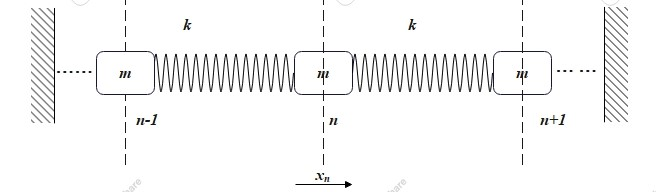
\includegraphics[width=1\textwidth]{Figures/N.jpg}
		\end{framed}
	\caption{ Linear chain of coupled $n$ mass oscillators .}
	\label{fig:N}
\end{figure}

After some time, all the particles of the system oscillate in harmonic oscillating motion with the same angular frequency of $\omega$, but different amplitudes and different
phases. Interestingly, only longitudinal motion (along the chain) in one dimension is considered. We will assume for the time being that all masses $(m)$ and spring constants $(k)$ are equal. Assuming up is the displacement ($x_n$) from equilibrium of mass $n$, then the equation of movements for each mass is given by following equations. 
Consider three adjacent particles with indexes $n - 1$, $n$ and $n + 1$ indicated by in the figure \ref{fig:N}. The equation of motion of the $n^{th}$, $(n-1)^{th}$ and $(n+1)^{th}$  of the particles which is given by,  

\begin{equation}
    m\Ddot{x_{n-1}} = k(2x_{n-1}+x_{n-2} + x_{n} )=0
\end{equation}

\begin{equation}
\label{Jo}
       m\Ddot{x_{n}} = k(x_{n-1}+2x_n - x_{n+1} )=0
\end{equation}

\begin{equation}
       m\Ddot{x_{n+1}} = k(x_{n-1}+ x_n - 2x_{n+1} )=0
\end{equation}

The periodic solutions to the equation of motion, so we might expect the solution to have the form.

\begin{equation}
\label{j1}
    x_{n-1} = Aexp[i(\omega t - k_p(c-1)d)]
\end{equation}

\begin{equation}
\label{j2}
    x_{n} = Aexp[i(\omega t - k_pcd)]
\end{equation}

\begin{equation}
\label{j3}
    x_{n+1} = Aexp[i(\omega t - k_p(c+1)d)]
\end{equation}

$A$ = number of particles in the system \\
$\omega$ = angular frequency \\
$k_p$ = propagation constant \\
$k$ = spring constant

Note that the mass are situated on equally spaced sites with a separation distance $d$. 

\subsection{Dispersion Relation}
\paragraph{}
The acceleration of a specific mass is determined not only by its own displacement, but also by the displacements of its neighbours. And also, the displacement of mass $n$ for a specific normal mode with frequency $\omega$ can be represented as  equation in \eqref{j2}. The coefficients $A$ give the amplitudes of the oscillations for the various masses $n$. Furthermore, substitution of equations \eqref{j1}, \eqref{j2} and \eqref{j3} into equation \eqref{Jo} results in,

\begin{equation}
    -m\omega^2 = k[(exp(ik_p d) + exp(-ik_P d)-2]
\end{equation}

\begin{equation}
    -m\omega^2 = 2k[cos(k_pd)-1]
\end{equation}

\begin{equation}
    \omega = \sqrt{\frac{4k}{m}}sin(\frac{k_pd}{2})
\end{equation}

\begin{equation}
    \omega_0 = \sqrt{\frac{4k}{m}}
\end{equation}

The maximum angular velocity is $\omega_0$. And  phase velocity is $v_p$ and maximum phase velocity we can say $v_{max}$ by substitution \eqref{vp}. 

\begin{equation}
\label{vp}
    v_P = \frac{\omega}{k_p}
\end{equation}

\begin{equation}
    v_{max} = v_0 = d\sqrt{\frac{k}{m}}
\end{equation}

In general, a wave is a superposition of its harmonic components. The envelope or the group of waves are seen to move forward with a velocity $d\omega /  dt$ which is termed the group velocity. 

\begin{equation}
    v_G = \frac{d\omega}{dt}
\end{equation}
\begin{equation}
    V_G = v_0 cos(\frac{k_p d}{2})
\end{equation}

\newpage

\section{Investigate  the two-dimensional spring motion: the mass m is free to move in the $XY$ plane}
\label{XY}
\paragraph{}

It is not insignificant to extend our view of oscillators to other dimensions. In the real world there are many applications that we can see corresponding two-dimensional (2D) systems. Furthermore, this section the two-dimensional spring motion which is about the mass m is free to move in the $xy$ plane will be discussed.

\subsection{Motion for 2D spring motion of a single mass}

\paragraph{}

To obtain the results of 2D spring motion of a single mass we are given a simple task. As early stated in this, the mass m is free to move in the $xy$ plane. It is attached to the solid walls by two unstretched massless springs of spring constant, $k$ aligned along the $x$-axis and by the unstretched massless springs of spring constant $k$ oriented along the $y$-axis. Which means a block (mass $m$) is attached to the sides of a square box by 4 springs. The initial length of each spring is $l$. Place the block (mass $m$) at (0,0). The box is placed horizontally on a frictionless surface (ignore gravity). Let $x(t),y(t)$ the position of the block in time. Considering the given initial conditions and parameters the motion of the mass in the $xy$ plane in the small oscillation approximation will be investigated.

 
\begin{table}[hbt!]
\begin{center}
    \begin{tabular}{|p{8cm}|p{2cm}|}
    \hline
    \textbf{Description of constant} & \textbf{Constant} 
    \\
    \hline
      Spring constant   & $k$ \\
      \hline
     Initial length of each string & $l$ \\
     \hline
     Single mass & $m$ \\
     \hline
     Position of the block in time $x$ direction & $x(t)$ \\
     \hline
     Position of the block in time $y$ direction & $y(t)$ \\
     \hline
    \end{tabular}
    \caption{Description of the constant}
    \label{tab1}
    \end{center}
\end{table}

In the given above table \ref{tab1} explained the meaning of each and each constants that we have been using during our experiment. The place of block (mass $m$) at position (0,0) shown as given below figure \ref{fig:8}. After the change of lengths of the springs when the block is removed from the central position despicts in figure \ref{fig:9}. 

\newpage

\begin{figure}[hbt!]
	\centering
	\begin{framed}
	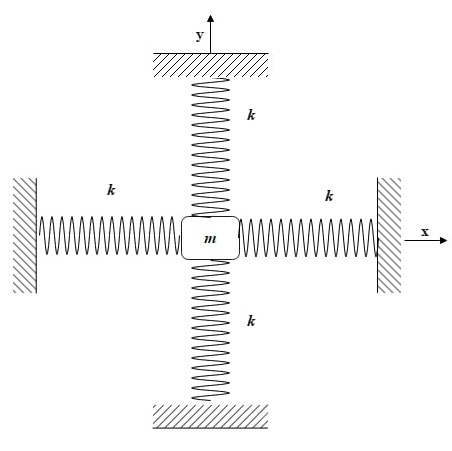
\includegraphics[width=0.5\textwidth]{Figures/H.jpeg}
	\end{framed}
	\caption{ The place of block (mass $m$) at position (0,0).}
	\label{fig:8}
\end{figure}

\begin{figure}[hbt!]
	\centering
	\begin{framed}
	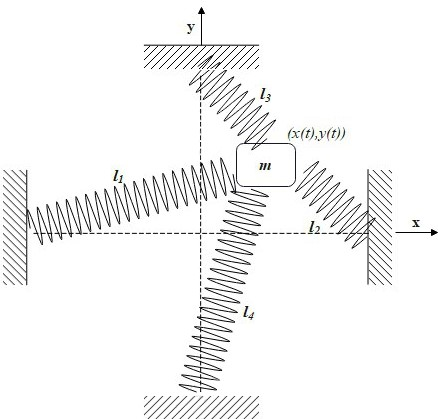
\includegraphics[width=0.53\textwidth]{Figures/I.jpeg}
	\end{framed}
	\caption{ The place of block (mass $m$) at position $(x(t),y(t))$.}
	\label{fig:9}
\end{figure}

\newpage 

Let's consider the stretched length of the given four strings. Those are called as $l_1,l_2,l_3$ and $l_4$ in respectively. 

\begin{equation}
    \label{s1}
    l^2_1 = (x+l)^2+y^2
\end{equation}

\begin{equation}
    \label{s2}
    l^2_2 = (x-l)^2+y^2
\end{equation}

\begin{equation}
    \label{s3}
    l^2_3 = (y+l)^2+x^2
\end{equation}

\begin{equation}
    \label{s4}
    l^2_4 = (y-l)^2+x^2
\end{equation}

Thus, $l_1,l_2,l_3$ and $l_4$ we can write as, 

\begin{equation}
    \label{s11}
    l_1 = \sqrt{(x+l)^2+y^2}
\end{equation}

\begin{equation}
    \label{s22}
    l_2 = \sqrt{(x-l)^2+y^2}
\end{equation}

\begin{equation}
    \label{s33}
    l_3 = \sqrt{(y+l)^2+x^2}
\end{equation}

\begin{equation}
    \label{s44}
    l_4 = \sqrt{(y-l)^2+x^2}
\end{equation}

Since we have stretched length of each springs $l_1,l_2,l_3$ and $l_4$, now we consider the each tension of which all are deforming during the experiment. Each of tension were defined as below. 


\begin{equation}
    \label{t1}
    F_1 = k(\sqrt{(x+l)^2+y^2}- l^2 )^2
\end{equation}

\begin{equation}
    \label{t2}
    F_2 = k(\sqrt{(x-l)^2+y^2}- l^2 )^2
\end{equation}

\begin{equation}
    \label{t3}
    F_3 = k(\sqrt{x^2+(y+l)^2}- l^2 )^2
\end{equation}

\begin{equation}
    \label{t4}
    F_4 = k(\sqrt{x^2+(y-l)^2}- l^2 )^2
\end{equation}

As early discussed, in this project we are not solving given tasks by using Newton's second law \cite{ghayesh2012nonlinear}. Therefore we have to use an alternative option which is called as Euler's lagrange equation. We discussed more details and much needed background about Euler's lagrange in section \ref{lag}. As early stated Euler's lagrange has two major components. Which is known as kinetic energy and potential energy. During the this kind of problems kinetic energy and potential energy play a major role. Therefore, before the solve obtained differential equations it would be prefer to look at governing equations (which may obtained using Euler's lagrange equations ) as much as possible. Because final outputs and their accuracy depend on the initial steps, what we have been used.  

\newpage 

\subsection{Equations of motion for 2D spring motion of a single mass}
\label{xo}

In this section, more details regarding Euler's lagrange equation, governing equations and scientific background about deriving relevant equations will be discussed. As mentioned earlier, before the obtain governing equations we have to be concerned about identifying kinetic energy and potential energy. Therefore, the terms of kinetic energy and potential energy are listed below. Let $V_1,V_2,V_3$ and $V_4$ are potential energies and $T$ is kinetic energy of particle (mass $m$). 

The kinetic energy due to the motion of the mass,

\begin{equation}
\label{k1}
    T = \frac{1}{2}m(\dot{x}^2 + \dot{y}^2)
\end{equation}

The potential energy due to the motion of the mass,

\begin{equation}
    \label{v1}
    V_1 = \frac{1}{2}k(\sqrt{(x+l)^2+y^2}- l^2 )^2
\end{equation}

\begin{equation}
    \label{v2}
    V_2 = \frac{1}{2}k(\sqrt{(x-l)^2+y^2}- l^2 )^2 
\end{equation}

\begin{equation}
    \label{v3}
    V_3 = \frac{1}{2}k(\sqrt{x^2+(y+l)^2}- l^2 )^2 
\end{equation}

\begin{equation}
    \label{v4}
    V_4 =  \frac{1}{2}k(\sqrt{x^2+(y-l)^2}- l^2 )^2
\end{equation}

Let, we can write total potential energy due to the motion of the particle (mass $m$) as shown equation \eqref{V}.

\begin{equation}
    V = V_1+V_2+V_3+V_4
\end{equation}

\begin{align}
\label{V}
\begin{split}
    V = \frac{1}{2}k(\sqrt{x^2+(y-l)^2}- l^2 )^2+ \frac{1}{2}k(\sqrt{(x+l)^2+y^2}- l^2 )^2 +  \frac{1}{2}k(\sqrt{x^2+(y+l)^2}- l^2 )^2    \\ + \frac{1}{2}k(\sqrt{(x-l)^2+y^2}- l^2 )^2 
    \end{split}
\end{align}

Then applying both equations \eqref{k1} and \eqref{V} into the lagrange equation \eqref{3}. 



\begin{align}
\label{L1}
    \begin{split}
        L = \frac{1}{2}m(\dot{x}^2 + \dot{y}^2) - \bigg ( \frac{1}{2}k(\sqrt{x^2+(y-l)^2}- l^2 )^2 + \\ \frac{1}{2}k(\sqrt{(x+l)^2+y^2}- l^2 )^2 + \\ \frac{1}{2}k(\sqrt{x^2+(y+l)^2}- l^2 )^2  + \\\frac{1}{2}k(\sqrt{(x-l)^2+y^2}- l^2 )^2 \bigg )
    \end{split}
\end{align}

In this special case (2D motion for 2D spring motion of a single mass) we have define lagrange equations as below. 

\begin{equation}
    \label{X}
    \frac{d}{dt}(\frac{\partial L}{\partial \dot{x}})-\frac{\partial L}{\partial x}  = 0 
\end{equation}

\begin{equation}
    \label{Y}
     \frac{d}{dt}(\frac{\partial L}{\partial \dot{y}})-\frac{\partial L}{\partial y} = 0
\end{equation}

First, consider both equation \eqref{L1} and equation \eqref{X} simultaneously to obtain motion of particle (mass $m$) direction to $x$.

\begin{align*}
  \frac{d}{dt}(\frac{\partial L}{\partial \dot{x}})-\frac{\partial L}{\partial x}  = 0  
\end{align*}

\begin{align}
\label{X1}
\begin{split}
      m \Dot{x} - \bigg[ \dfrac{kx\left(\sqrt{x^2+\left(y-l\right)^2}-l^2\right)}{\sqrt{x^2+\left(y-l\right)^2}} +   { \dfrac{k\left(x+l\right)\left(\sqrt{\left(x+l\right)^2+y^2}-l^2\right)}{\sqrt{\left(x+l\right)^2+y^2}}
} +  \dfrac{kx\left(\sqrt{x^2+\left(y+l\right)^2}-l^2\right)}{\sqrt{x^2+\left(y+l\right)^2}} \\ + \dfrac{k\left(\sqrt{\left(x-l\right)^2+y^2}-l^2\right)^2}{2}
\bigg]& = 0 
    \end{split}
\end{align}

After that, consider both equation \eqref{L1} and equation \eqref{Y} simultaneously to obtain motion of particle (mass $m$) direction to $y$.

\begin{align*}
   \frac{d}{dt}(\frac{\partial L}{\partial \dot{y}})-\frac{\partial L}{\partial y} = 0
\end{align*}


\begin{align}
\label{Y1}
    \begin{split}
          m \Dot{y} - \bigg[ \dfrac{k\left(y-l\right)\left(\sqrt{\left(y-l\right)^2+x^2}-l^2\right)}{\sqrt{\left(y-l\right)^2+x^2}}  + \dfrac{ky\left(\sqrt{y^2+\left(x+l\right)^2}-l^2\right)}{\sqrt{y^2+\left(x+l\right)^2}} + \dfrac{k\left(y+l\right)\left(\sqrt{\left(y+l\right)^2+x^2}-l^2\right)}{\sqrt{\left(y+l\right)^2+x^2}}\\+ \dfrac{ky\left(\sqrt{y^2+\left(x-l\right)^2}-l^2\right)}{\sqrt{y^2+\left(x-l\right)^2}}
\bigg]& = 0   \\
    \end{split}
\end{align}

\newpage

The tension in the first spring of length $l_1$ is $F_1 \approx k (a+ x – l) = kx$. Magnitude of  $x$-component of this tension is $F_1 cosθ_1 \approx F_1 = kx$ since the angle $\theta_1$ made by $l_1$ with the x-axis is small. Therefore, we find that the x-component of the return force is entirely due to the two springs of lengths $l_1$ and $l_2$. 
\begin{equation}
    F_x = -2kx
\end{equation}

The two springs of lengths $l_3$ and $l_4$ are also totally responsible for the y-component of the return force,

\begin{equation}
     F_y = -2ky
\end{equation}

As a result,  two uncoupled differential equations for the mass m along the x- and y-axes were obtained as below shown.

\begin{equation}
    m\Ddot{x} = -2kx
\end{equation}

\begin{equation}
    m\Ddot{y} = -2ky
\end{equation}

The solutions of these two equations were determined as shown in equations \eqref{so1} and \eqref{so2}.

\begin{equation}
    \label{so1}
    x = A cos(\omega t + \delta_1)
\end{equation}

\begin{equation}
    \label{so2}
    Y = B cos(\omega t + \delta_2)
\end{equation}

In here, $A$, $B$, $\delta_1$, and $\delta_2$ are arbitrary integration constants. We can significantly shorten the previous equations by changing the origin of time. 

\begin{equation}
t\rightarrow t' + \delta_1/\omega
\end{equation}

Hence, we obtain,

\begin{equation}
\label{f1}
    x = A\,\cos(\omega\,t')
\end{equation}

\begin{equation}
\label{f2}
    y = B\,\cos(\omega\,t'-\Delta)
\end{equation}

where ${\mit\Delta}=\phi_2-\phi_1$. 

It is important to note that the motion is obviously periodic in time, with a period of $T=2\pi/ \omega$. As a result, the particle must follow a closed route in the $x$-$y$ plane.














%\chapter{Methodology}
\label{chap:03}
\paragraph{}

Several ideas must be known in order to determine dynamic vibration analysis. There are several elements that impact which model is applied and understood. To determine which model to utilise, the complexity of the system and the number of influencing parameters must be determined. This chapter will go over the different coupled spring mass systems oscillations vibration involving many objects (usually without damping or driving) and how they behave with different parameter values, as well as complex analysis using the Runge Kutta fourth order method (section \ref{RK}) and how to obtain the numerical analysis using software MATLAB. Roughly working, the count of the degree of freedom goes as follows: two and $n^{th}$ for linear systems. To obtain vibration of the two dimensional (2D) spring mass system, which has  one mass and  $n^{th}$ mass respectively. 




\section{Investigate the motion for undamped linear spring mass system with  coupled two degrees of freedom}
\label{2DOF}

The simple one degree of freedom (1DOF) \cite{tsai2020design} systems examined in the preceding section are pretty helpful in developing an understanding of the general properties of vibrating systems. They are far too simplistic to approximate the majority of real-world systems. Real systems have multiple degrees of freedom. Real-world systems are almost never linear. It turns out that they are, but you will not be convinced unless you know how to evaluate more genuine issues and notice how they frequently behave just like the simple idealizations. As early stated in this section spring system of two degrees of freedom (2DOF) \cite{eiss1964vibration} will be discussed with details. 

\subsection{Equations of motion for undamped linear spring mass system with 2DOF }

\paragraph{}
Newton’s second law of motion tells us how a point mass moves in response to a force. But as early stated in this project we use only Lagrange equation (section \ref{lag}) to obtain the equations of motion given coupled systems. In this section, we are given two masses, each of mass $m_1$ and $m_2$, sitting on a frictionless horizontal surface.  The blocks are attached to three springs, and the outer springs are also attached to stationary walls, as shown in figure \ref{fig:7}. The two outer springs each have force constant $k_1$ and $k_3$ respectively, and the inner spring has force constant $k_2$. When the blocks are at rest the springs are unstretched.

Let $_1$ and $x_2$ represent the displacements of mass 1 and 2 from their equilibrium locations, positive to the right. Our goal is to determine the differential equations of motion for each mass and then solve them to determine $x_1(t)$ and $x_2 (t)$. In given figure \ref{fig:6} Degree of freedom (DOF) = 3$\times$2-4 =2 from equation \eqref{1}. Therefore we can say in the figure \ref{fig:6} has two body degree of freedom.



 \begin{figure}[hbt!]
	\centering
	\begin{framed}
	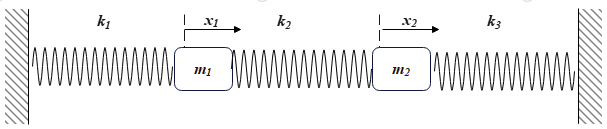
\includegraphics[width=0.7\textwidth]{Figures/G.png}
		\end{framed}
	\caption{ Undamped linear spring mass systems with 2DOF.}
	\label{fig:7}
\end{figure}

In the section, given figure \ref{fig:6} is a two degree of freedom system (2DOF), governed by two differential equations. The governing equations can also be achieved by following Lagrange's Equation directly. The expression for kinetic energy is,

\begin{equation}
    T = \frac{1}{2}m_1\dot{x_1}^2 + \frac{1}{2}m_2\dot{x_2}^2
\end{equation}
And also, the expression for potential energy is,
\begin{equation}
    V = \frac{1}{2}k_1x^2+\frac{1}{2}k_2(x_2-x_1)^2+\frac{1}{2}k_3x_3^2
\end{equation}

 Consider the following seemingly silly combination of the kinetic and potential energies ($T$ and $V$ , respectively), It is denoted by $L$,
\begin{equation}
\label{aaa}
    L = T-V
\end{equation}


Applying Lagrange’s equation to equation \eqref{aaa},
\begin{equation}
    \frac{d}{dt}(\frac{\partial L}{\partial \dot{x1}})-\frac{\partial L}{\partial x1} = 0 
\end{equation}
\begin{equation}
     \frac{d}{dt}(\frac{\partial L}{\partial \dot{x2}})-\frac{\partial L}{\partial x2} = 0
\end{equation}

Governing differential equations \cite{cartwright1945non} are based on balance laws for mass and momentum, and completed by constitutive relations for the fluid and solid phases as well as their mutual interactions. In the section  equation \eqref{aaa} its results we can obtain the governing equations as,

\newpage

\begin{equation}
\label{aab}
    m_1\dot{x_1}+(k_1+k_2)x_1-k_2x_2=0
\end{equation}
\begin{equation}
\label{aac}
    m_2\dot{x_2}-k_2x_1+(k_2+k_3)x_2 = 0
\end{equation}

Clearly,  we were able to realised for multi degree of freedom systems, this approach (Lagrangian) has advantages over the force balancing approach using Newton’s law.

\subsection{Matrix form of equations of motion}

\paragraph{}

To approach vibration problems, we always put the equations of motion (\eqref{aab} and \eqref{aac}) in matrix form. The matrix form of the system of governing equations of motion is as follows and the component matrices are commonly named as listed below. 
\begin{equation}
    M \frac{d\dot{x^2}}{dt}+ Kx = 0
\end{equation}

\begin{equation}
\label{aad}
    [M]{\dot{X}}+[K]{X} = 0
\end{equation}

\begin{gather}
 \begin{bmatrix} m_1 & 0 \\ 0 & m_2 \end{bmatrix} \frac{d^2}{dt^2} \begin{bmatrix}
  x_1 \\ x_2
 \end{bmatrix} + \begin{bmatrix}
  k_1+k_2 & -k_2 \\ -k_2 & k_2+k_3
 \end{bmatrix}
 \begin{bmatrix}
  x_1 \\ x_2
 \end{bmatrix}
 =
  \begin{bmatrix}
0 \\0
   \end{bmatrix}
\end{gather}

\begin{gather}
    \begin{bmatrix}
m_1 & 0\\0& m_2 
\end{bmatrix}{\dot{X}} +
\begin{bmatrix}
k_1+k_2 &-k_2\\-k_2&k_2+k_3
\end{bmatrix}{X} = 0
\end{gather}


Where $x$ is a vector of the variables describing the motion,  $M$ is called the ‘mass matrix’ and $K$ is called the ‘Stiffness matrix’ for the system. $M$ and $K$ are 2$\times$2 matrices for a system with two masses (or, more broadly, two degrees of freedom). They are $n \times n$ matrices for a system with $n$ degrees of freedom.

\subsection{Natural frequencies and mode shapes for 2-degrees-of-freedom undamped linear system}
\paragraph{}

First. now let us go over the definitions of natural frequencies and mode shapes first. Remember that we may make a system vibrate by slightly pushing it from its static equilibrium state and then releasing it. The resulting motion will not be harmonic in general. Certain special initial displacements, on the other hand, will result in harmonic vibrations. These unique initial deflections are known as mode shapes, and the accompanying vibrational frequencies are known as natural frequencies \cite{kuether2014numerical} \cite{gigerenzer2011natural}. A vibrating system's natural frequencies are its most essential attribute. It is useful to have a straightforward method for calculating them.

To continue, we need to make the crucial assumption that the system has specific motions in which both masses oscillate at the same frequency. We will observe that for one-dimensional chains, there seem to be exactly as many normal modes as there are masses in the system. Each and every normal mode corresponds to a single frequency of motion, but the frequencies of normal modes can be vary. We may represent the general motion of any mass in terms of a superposition of normal modes once we have identified the movements associated with the normal modes and determined the normal mode frequencies. Assume that both masses move at the same frequency to find the normal mode frequencies.

\begin{equation}
\label{x1}
    x_1 = A_1e^{i\omega t}
\end{equation}

\begin{equation}
\label{x2}
    x_2 = A_2e^{i\omega t}
\end{equation}

Consider the double derivation of equation \eqref{x1} and \eqref{x2},

\begin{equation}
\label{x1}
    \Ddot{x_1}  = - \omega^2 A_1e^{i\omega t} = -\omega^2 x_1
\end{equation}

\begin{equation}
\label{x2}
   \Ddot{x_2}  = - \omega^2 A_2e^{i\omega t} = -\omega^2 x_2
\end{equation}
 
Where $A_1$ and $A_2$ are arbitrary constants.
 
Substituting these into the equations of motion \eqref{aab} and \eqref{aac}  gives us,

\begin{equation}
\label{x3}
    -\omega^2 m_1 A_1e^{i\omega t} +(k_1 + k_2) A_1e^{i\omega t}- k_2A_2e^{i\omega t}= 0
\end{equation}

\begin{equation}
    \label{x4}
    -\omega^2 m_2 A_2e^{i\omega t} - k_2 A_1 e^{i\omega t} + (k_2 + k_3)A_2e^{i\omega t} = 0 
\end{equation}

From equation \eqref{x3} and \eqref{x4}, since the exponential factor is common to all terms, we omit it and simplify, 

\begin{equation}
\label{x5}
    (\omega^2 m_1  -(k_1 + k_2)) A_1e^{i\omega t}+ k_2A_2e^{i\omega t}= 0
\end{equation}

\begin{equation}
    \label{x6}
   k_2 A_1 e^{i\omega t}  +(\omega^2 m_2  - (k_2 + k_3))A_2e^{i\omega t} = 0 
\end{equation}

And in matrix representation,

\begin{gather}
    \begin{bmatrix}
(\omega^2 m_1  -(k_1 + k_2)) & k_2\\k_2& (\omega^2 m_2  - (k_2 + k_3))
\end{bmatrix}\begin{bmatrix}
A_1 \\ A_2
\end{bmatrix}
 = 0
\end{gather}


For arbitrary frequencies the only solution of the equation is the “trivial” solution $A_1 = A_2 = 0$,  where both blocks remain at rest at their equilibrium positions. But from linear algebra we know that with just the right choice(s) of $\omega$ there are also non-trivial solution(s) if and only if the determinant of the coefficients vanishes, i.e., if and only if, 

\begin{gather}
    \begin{vmatrix}
(\omega^2 m_1  -(k_1 + k_2)) & k_2 \\
k_2 & (\omega^2 m_2  - (k_2 + k_3))
\end{vmatrix} = 0
\end{gather}

\begin{equation}
   \left( {{\omega ^2} - \frac{{{k_1} + {k_2}}}{{{m_1}}}} \right) \left( {{\omega ^2} - \frac{{{k_2} + {k_3}}}{{{m_2}}}} \right) - \frac{{k_2^2}}{{{m_1}{m_2}}} = 0
\end{equation}

\begin{equation}
    {\omega ^4} - \frac{{{k_1} + {k_2}}}{{{m_1}}}{\omega ^2} - \frac{{{k_2} + {k_3}}}{{{m_2}}}{\omega ^2}
+ \frac{{\left( {{k_1} + {k_2}} \right)\left( {{k_2} + {k_3}} \right)}}{{{m_1}{m_2}}} - \frac{{k_2^2}}{{{m_1}{m_2}}} = 0
\end{equation}

\begin{equation}
    {\omega ^4} - \left( {\frac{{{k_1} + {k_2}}}{{{m_1}}} + \frac{{{k_2} + {k_3}}}{{{m_2}}}} \right){\omega ^2}
+ \frac{{\left( {{k_1} + {k_2}} \right)\left( {{k_2} + {k_3}} \right)}}{{{m_1}{m_2}}} - \frac{{k_2^2}}{{{m_1}{m_2}}} = 0
\end{equation}

Finding solution this biquadratic equation, we find the eigen frequencies. Let us first obtain the discriminant. 

\begin{equation}
    D = {\left( {\frac{{{k_1} + {k_2}}}{{{m_1}}} + \frac{{{k_2} + {k_3}}}{{{m_2}}}} \right)^2}
- 4\left[ {\frac{{\left( {{k_1} + {k_2}} \right)\left( {{k_2} + {k_3}} \right)}}{{{m_1}{m_2}}} - \frac{{k_2^2}}{{{m_1}{m_2}}}} \right]
\end{equation}

\begin{equation}
    D ={\left( {\frac{{{k_1} + {k_2}}}{{{m_1}}}} \right)^2} + {\left( {\frac{{{k_2} + {k_3}}}{{{m_2}}}} \right)^2}
+ \frac{{2\left( {{k_1} + {k_2}} \right)\left( {{k_2} + {k_3}} \right)}}{{{m_1}{m_2}}}
- \frac{{4\left( {{k_1} + {k_2}} \right)\left( {{k_2} + {k_3}} \right)}}{{{m_1}{m_2}}}
+ \frac{{4k_2^2}}{{{m_1}{m_2}}}
\end{equation}

\begin{equation}
    D = {\left( {\frac{{{k_1} + {k_2}}}{{{m_1}}} - \frac{{{k_2} + {k_3}}}{{{m_2}}}} \right)^2}
+ \frac{{4k_2^2}}{{{m_1}{m_2}}}
\end{equation}

The formula will then explain the square of the eigen frequencies.

\begin{equation}
    {\omega ^2} = \frac{1}{2}\left\{ {\left( {\frac{{{k_1} + {k_2}}}{{{m_1}}} + \frac{{{k_2} + {k_3}}}{{{m_2}}}} \right) \pm {{\left[ {{{\left( {\frac{{{k_1} + {k_2}}}{{{m_1}}} - \frac{{{k_2} + {k_3}}}{{{m_2}}}} \right)}^2} + \frac{{4k_2^2}}{{{m_1}{m_2}}}} \right]}^{\frac{1}{2}}}} \right\}
\end{equation}

To prevent complicated formulas, we now consider the simpler case in which the stiffness of all springs is the same: ${k_1} = {k_2} ={k_3} = k$. And also mass ratio was introduced as: $\mu  = {\frac{{{m_2}}}{{{m_1}}}}.$ Then perhaps the equation for the square of oscillation frequency takes the form as this given equation \eqref{W2}.

\begin{equation}
    {\omega ^2} = \frac{1}{2}\left[ {\left( {\frac{{2k}}{{{m_1}}} + \frac{{2k}}{{{m_2}}}} \right) \pm \sqrt {{{\left( {\frac{{2k}}{{{m_1}}} - \frac{{2k}}{{{m_2}}}} \right)}^2} + \frac{{4{k^2}}}{{{m_1}{m_2}}}} } \right] 
\end{equation}

\begin{equation}
    \label{W1}
   {\omega ^2} = k\left[ {\left( {\frac{1}{{{m_1}}} + \frac{1}{{{m_2}}}} \right) \pm \sqrt {{{\left( {\frac{1}{{{m_1}}} - \frac{1}{{{m_2}}}} \right)}^2} + \frac{1}{{{m_1}{m_2}}}} } \right] 
\end{equation}

\begin{equation}
\label{W2}
  {\omega ^2}  = \frac{k}{{{m_2}}}\left[ {\mu  + 1 \pm \sqrt {{{\left( {\mu  - 1} \right)}^2} + \mu } } \right]
\end{equation}

The  earlier obtained expression \eqref{W1} and \eqref{W2} describe  eigen frequencies, ${\omega _1}$ (with the plus sign) and ${\omega _2}$ (with the minus sign). The following  formulas \eqref{w1} and \eqref{w2} describe  the eigen frequencies in the case of equal masses $\left( {\mu  = 1} \right)$.  


\begin{equation}
\label{w1}
    {\omega _1} = \sqrt {\frac{{3k}}{m}} 
\end{equation}

\begin{equation}
\label{w2}
    {\omega _2} = \sqrt {\frac{k}{m}} 
\end{equation}



The eigen frequencies actually depend on the $\left( {\mu } \right)$. Let's consider how it could be determined by using the $\mu$ values. It should be noted that the frequencies $(\omega_1 )$ and $(\omega_1 )$ have always been real numbers. This is a result of general physical concerns. Consequently, in the scenario of the imaginary frequency, there would be energy leakage, which defies the system's energy conservation assumption. This fact, on the other hand, can be proven mathematically. In actuality, the question simply pertains to frequency $\omega_2$.



The condition for non-negativity ${\omega _2}^2$ is stated by, 

\begin{equation}
\label{om1}
   \omega _2^2 > 0
\end{equation}

Applying \eqref{W2} into the equation \eqref{om1}.

\begin{equation}
\Rightarrow \mu + 1 - \sqrt {{{\left( {\mu - 1} \right)}^2} + \mu } > 0 
\end{equation}

\begin{equation}
    \Rightarrow \mu + 1 > \sqrt {{{\left( {\mu - 1} \right)}^2} + \mu}  
\end{equation}

The inequality's left side and the expression under the square root's right side are always positive. After squaring both sides, we obtain. 

\begin{equation}
    {\left( {\mu + 1} \right)^2} > {\left( {\mu - 1} \right)^2} + \mu 
\end{equation}

\begin{equation}
\Rightarrow \cancel{\mu ^2} + 2\mu + \cancel{1} > \cancel{\mu ^2} - 2\mu + \cancel{1} + \mu 
\end{equation}

\begin{equation}
    \Rightarrow 3\mu > 0 
\end{equation}

\begin{equation}
    \Rightarrow \mu > 0
\end{equation}

Consequently which always holds the requirements.



\section{Investigate the motion for undamped linear spring mass system with coupled many degrees of freedom}
\label{XY2}

\paragraph{}

Substances are made up of a large number of less or more organised fundamental components such as molecules, atoms, or ions. Solids and liquids are formed by particles that have a strong enough attraction to one another to form a compact entity \cite{chaudhari2016molecular}. Each and every component of a solid or liquid substance has an equilibrium condition that is determined by the force of the particles around it. The equilibrium position correlates to the minimal potential energy, and each particle oscillates around the minimum potential energy \cite{guvench2008comparison}. As an example. we will utilise an infinite chain of bonded particles arranged in a single line as a simplified crystal model.

\subsection{Equations of motion for many degree of freedom spring mass system}

\paragraph{}
In the previous section we considered only motion of two degrees of freedom spring mass system. Inside this section, we will rapidly show that the identical equations that we discovered in the previous section also apply to longitudinal waves. To examine the behavior of vibrational motion in an infinite one dimension (1D) chain of diatomic masses \cite{chen2020active},we suppose that the distance between the equilibrium position of nearest-neighboring masses is a such that the total number of masses $n$ in the chain is very large. The $x$-axis is supposed to run through the 1D-chain of masses \cite{lucovsky1970extension}. Consider the given figure \ref{fig:N} a horizontal spring system with $n$ masses connected by comparable springs and a spring constant $k$. 

 \begin{figure}[hbt!]
	\centering
	\begin{framed}
	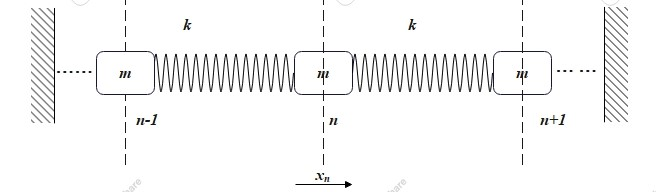
\includegraphics[width=1\textwidth]{Figures/N.jpg}
		\end{framed}
	\caption{ Linear chain of coupled $n$ mass oscillators .}
	\label{fig:N}
\end{figure}

After some time, all the particles of the system oscillate in harmonic oscillating motion with the same angular frequency of $\omega$, but different amplitudes and different
phases. Interestingly, only longitudinal motion (along the chain) in one dimension is considered. We will assume for the time being that all masses $(m)$ and spring constants $(k)$ are equal. Assuming up is the displacement ($x_n$) from equilibrium of mass $n$, then the equation of movements for each mass is given by following equations. 
Consider three adjacent particles with indexes $n - 1$, $n$ and $n + 1$ indicated by in the figure \ref{fig:N}. The equation of motion of the $n^{th}$, $(n-1)^{th}$ and $(n+1)^{th}$  of the particles which is given by,  

\begin{equation}
    m\Ddot{x_{n-1}} = k(2x_{n-1}+x_{n-2} + x_{n} )=0
\end{equation}

\begin{equation}
\label{Jo}
       m\Ddot{x_{n}} = k(x_{n-1}+2x_n - x_{n+1} )=0
\end{equation}

\begin{equation}
       m\Ddot{x_{n+1}} = k(x_{n-1}+ x_n - 2x_{n+1} )=0
\end{equation}

The periodic solutions to the equation of motion, so we might expect the solution to have the form.

\begin{equation}
\label{j1}
    x_{n-1} = Aexp[i(\omega t - k_p(c-1)d)]
\end{equation}

\begin{equation}
\label{j2}
    x_{n} = Aexp[i(\omega t - k_pcd)]
\end{equation}

\begin{equation}
\label{j3}
    x_{n+1} = Aexp[i(\omega t - k_p(c+1)d)]
\end{equation}

$A$ = number of particles in the system \\
$\omega$ = angular frequency \\
$k_p$ = propagation constant \\
$k$ = spring constant

Note that the mass are situated on equally spaced sites with a separation distance $d$. 

\subsection{Dispersion Relation}
\paragraph{}
The acceleration of a specific mass is determined not only by its own displacement, but also by the displacements of its neighbours. And also, the displacement of mass $n$ for a specific normal mode with frequency $\omega$ can be represented as  equation in \eqref{j2}. The coefficients $A$ give the amplitudes of the oscillations for the various masses $n$. Furthermore, substitution of equations \eqref{j1}, \eqref{j2} and \eqref{j3} into equation \eqref{Jo} results in,

\begin{equation}
    -m\omega^2 = k[(exp(ik_p d) + exp(-ik_P d)-2]
\end{equation}

\begin{equation}
    -m\omega^2 = 2k[cos(k_pd)-1]
\end{equation}

\begin{equation}
    \omega = \sqrt{\frac{4k}{m}}sin(\frac{k_pd}{2})
\end{equation}

\begin{equation}
    \omega_0 = \sqrt{\frac{4k}{m}}
\end{equation}

The maximum angular velocity is $\omega_0$. And  phase velocity is $v_p$ and maximum phase velocity we can say $v_{max}$ by substitution \eqref{vp}. 

\begin{equation}
\label{vp}
    v_P = \frac{\omega}{k_p}
\end{equation}

\begin{equation}
    v_{max} = v_0 = d\sqrt{\frac{k}{m}}
\end{equation}

In general, a wave is a superposition of its harmonic components. The envelope or the group of waves are seen to move forward with a velocity $d\omega /  dt$ which is termed the group velocity. 

\begin{equation}
    v_G = \frac{d\omega}{dt}
\end{equation}
\begin{equation}
    V_G = v_0 cos(\frac{k_p d}{2})
\end{equation}

\newpage

\section{Investigate  the two-dimensional spring motion: the mass m is free to move in the $XY$ plane}
\label{XY}
\paragraph{}

It is not insignificant to extend our view of oscillators to other dimensions. In the real world there are many applications that we can see corresponding two-dimensional (2D) systems. Furthermore, this section the two-dimensional spring motion which is about the mass m is free to move in the $xy$ plane will be discussed.

\subsection{Motion for 2D spring motion of a single mass}

\paragraph{}

To obtain the results of 2D spring motion of a single mass we are given a simple task. As early stated in this, the mass m is free to move in the $xy$ plane. It is attached to the solid walls by two unstretched massless springs of spring constant, $k$ aligned along the $x$-axis and by the unstretched massless springs of spring constant $k$ oriented along the $y$-axis. Which means a block (mass $m$) is attached to the sides of a square box by 4 springs. The initial length of each spring is $l$. Place the block (mass $m$) at (0,0). The box is placed horizontally on a frictionless surface (ignore gravity). Let $x(t),y(t)$ the position of the block in time. Considering the given initial conditions and parameters the motion of the mass in the $xy$ plane in the small oscillation approximation will be investigated.

 
\begin{table}[hbt!]
\begin{center}
    \begin{tabular}{|p{8cm}|p{2cm}|}
    \hline
    \textbf{Description of constant} & \textbf{Constant} 
    \\
    \hline
      Spring constant   & $k$ \\
      \hline
     Initial length of each string & $l$ \\
     \hline
     Single mass & $m$ \\
     \hline
     Position of the block in time $x$ direction & $x(t)$ \\
     \hline
     Position of the block in time $y$ direction & $y(t)$ \\
     \hline
    \end{tabular}
    \caption{Description of the constant}
    \label{tab1}
    \end{center}
\end{table}

In the given above table \ref{tab1} explained the meaning of each and each constants that we have been using during our experiment. The place of block (mass $m$) at position (0,0) shown as given below figure \ref{fig:8}. After the change of lengths of the springs when the block is removed from the central position despicts in figure \ref{fig:9}. 

\newpage

\begin{figure}[hbt!]
	\centering
	\begin{framed}
	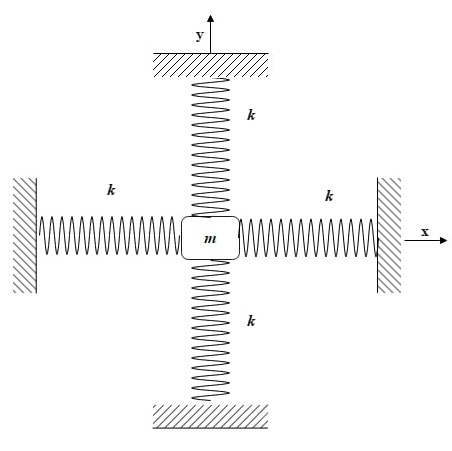
\includegraphics[width=0.5\textwidth]{Figures/H.jpeg}
	\end{framed}
	\caption{ The place of block (mass $m$) at position (0,0).}
	\label{fig:8}
\end{figure}

\begin{figure}[hbt!]
	\centering
	\begin{framed}
	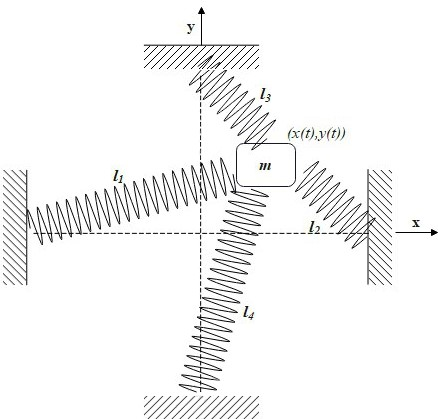
\includegraphics[width=0.53\textwidth]{Figures/I.jpeg}
	\end{framed}
	\caption{ The place of block (mass $m$) at position $(x(t),y(t))$.}
	\label{fig:9}
\end{figure}

\newpage 

Let's consider the stretched length of the given four strings. Those are called as $l_1,l_2,l_3$ and $l_4$ in respectively. 

\begin{equation}
    \label{s1}
    l^2_1 = (x+l)^2+y^2
\end{equation}

\begin{equation}
    \label{s2}
    l^2_2 = (x-l)^2+y^2
\end{equation}

\begin{equation}
    \label{s3}
    l^2_3 = (y+l)^2+x^2
\end{equation}

\begin{equation}
    \label{s4}
    l^2_4 = (y-l)^2+x^2
\end{equation}

Thus, $l_1,l_2,l_3$ and $l_4$ we can write as, 

\begin{equation}
    \label{s11}
    l_1 = \sqrt{(x+l)^2+y^2}
\end{equation}

\begin{equation}
    \label{s22}
    l_2 = \sqrt{(x-l)^2+y^2}
\end{equation}

\begin{equation}
    \label{s33}
    l_3 = \sqrt{(y+l)^2+x^2}
\end{equation}

\begin{equation}
    \label{s44}
    l_4 = \sqrt{(y-l)^2+x^2}
\end{equation}

Since we have stretched length of each springs $l_1,l_2,l_3$ and $l_4$, now we consider the each tension of which all are deforming during the experiment. Each of tension were defined as below. 


\begin{equation}
    \label{t1}
    F_1 = k(\sqrt{(x+l)^2+y^2}- l^2 )^2
\end{equation}

\begin{equation}
    \label{t2}
    F_2 = k(\sqrt{(x-l)^2+y^2}- l^2 )^2
\end{equation}

\begin{equation}
    \label{t3}
    F_3 = k(\sqrt{x^2+(y+l)^2}- l^2 )^2
\end{equation}

\begin{equation}
    \label{t4}
    F_4 = k(\sqrt{x^2+(y-l)^2}- l^2 )^2
\end{equation}

As early discussed, in this project we are not solving given tasks by using Newton's second law \cite{ghayesh2012nonlinear}. Therefore we have to use an alternative option which is called as Euler's lagrange equation. We discussed more details and much needed background about Euler's lagrange in section \ref{lag}. As early stated Euler's lagrange has two major components. Which is known as kinetic energy and potential energy. During the this kind of problems kinetic energy and potential energy play a major role. Therefore, before the solve obtained differential equations it would be prefer to look at governing equations (which may obtained using Euler's lagrange equations ) as much as possible. Because final outputs and their accuracy depend on the initial steps, what we have been used.  

\newpage 

\subsection{Equations of motion for 2D spring motion of a single mass}
\label{xo}

In this section, more details regarding Euler's lagrange equation, governing equations and scientific background about deriving relevant equations will be discussed. As mentioned earlier, before the obtain governing equations we have to be concerned about identifying kinetic energy and potential energy. Therefore, the terms of kinetic energy and potential energy are listed below. Let $V_1,V_2,V_3$ and $V_4$ are potential energies and $T$ is kinetic energy of particle (mass $m$). 

The kinetic energy due to the motion of the mass,

\begin{equation}
\label{k1}
    T = \frac{1}{2}m(\dot{x}^2 + \dot{y}^2)
\end{equation}

The potential energy due to the motion of the mass,

\begin{equation}
    \label{v1}
    V_1 = \frac{1}{2}k(\sqrt{(x+l)^2+y^2}- l^2 )^2
\end{equation}

\begin{equation}
    \label{v2}
    V_2 = \frac{1}{2}k(\sqrt{(x-l)^2+y^2}- l^2 )^2 
\end{equation}

\begin{equation}
    \label{v3}
    V_3 = \frac{1}{2}k(\sqrt{x^2+(y+l)^2}- l^2 )^2 
\end{equation}

\begin{equation}
    \label{v4}
    V_4 =  \frac{1}{2}k(\sqrt{x^2+(y-l)^2}- l^2 )^2
\end{equation}

Let, we can write total potential energy due to the motion of the particle (mass $m$) as shown equation \eqref{V}.

\begin{equation}
    V = V_1+V_2+V_3+V_4
\end{equation}

\begin{align}
\label{V}
\begin{split}
    V = \frac{1}{2}k(\sqrt{x^2+(y-l)^2}- l^2 )^2+ \frac{1}{2}k(\sqrt{(x+l)^2+y^2}- l^2 )^2 +  \frac{1}{2}k(\sqrt{x^2+(y+l)^2}- l^2 )^2    \\ + \frac{1}{2}k(\sqrt{(x-l)^2+y^2}- l^2 )^2 
    \end{split}
\end{align}

Then applying both equations \eqref{k1} and \eqref{V} into the lagrange equation \eqref{3}. 



\begin{align}
\label{L1}
    \begin{split}
        L = \frac{1}{2}m(\dot{x}^2 + \dot{y}^2) - \bigg ( \frac{1}{2}k(\sqrt{x^2+(y-l)^2}- l^2 )^2 + \\ \frac{1}{2}k(\sqrt{(x+l)^2+y^2}- l^2 )^2 + \\ \frac{1}{2}k(\sqrt{x^2+(y+l)^2}- l^2 )^2  + \\\frac{1}{2}k(\sqrt{(x-l)^2+y^2}- l^2 )^2 \bigg )
    \end{split}
\end{align}

In this special case (2D motion for 2D spring motion of a single mass) we have define lagrange equations as below. 

\begin{equation}
    \label{X}
    \frac{d}{dt}(\frac{\partial L}{\partial \dot{x}})-\frac{\partial L}{\partial x}  = 0 
\end{equation}

\begin{equation}
    \label{Y}
     \frac{d}{dt}(\frac{\partial L}{\partial \dot{y}})-\frac{\partial L}{\partial y} = 0
\end{equation}

First, consider both equation \eqref{L1} and equation \eqref{X} simultaneously to obtain motion of particle (mass $m$) direction to $x$.

\begin{align*}
  \frac{d}{dt}(\frac{\partial L}{\partial \dot{x}})-\frac{\partial L}{\partial x}  = 0  
\end{align*}

\begin{align}
\label{X1}
\begin{split}
      m \Dot{x} - \bigg[ \dfrac{kx\left(\sqrt{x^2+\left(y-l\right)^2}-l^2\right)}{\sqrt{x^2+\left(y-l\right)^2}} +   { \dfrac{k\left(x+l\right)\left(\sqrt{\left(x+l\right)^2+y^2}-l^2\right)}{\sqrt{\left(x+l\right)^2+y^2}}
} +  \dfrac{kx\left(\sqrt{x^2+\left(y+l\right)^2}-l^2\right)}{\sqrt{x^2+\left(y+l\right)^2}} \\ + \dfrac{k\left(\sqrt{\left(x-l\right)^2+y^2}-l^2\right)^2}{2}
\bigg]& = 0 
    \end{split}
\end{align}

After that, consider both equation \eqref{L1} and equation \eqref{Y} simultaneously to obtain motion of particle (mass $m$) direction to $y$.

\begin{align*}
   \frac{d}{dt}(\frac{\partial L}{\partial \dot{y}})-\frac{\partial L}{\partial y} = 0
\end{align*}


\begin{align}
\label{Y1}
    \begin{split}
          m \Dot{y} - \bigg[ \dfrac{k\left(y-l\right)\left(\sqrt{\left(y-l\right)^2+x^2}-l^2\right)}{\sqrt{\left(y-l\right)^2+x^2}}  + \dfrac{ky\left(\sqrt{y^2+\left(x+l\right)^2}-l^2\right)}{\sqrt{y^2+\left(x+l\right)^2}} + \dfrac{k\left(y+l\right)\left(\sqrt{\left(y+l\right)^2+x^2}-l^2\right)}{\sqrt{\left(y+l\right)^2+x^2}}\\+ \dfrac{ky\left(\sqrt{y^2+\left(x-l\right)^2}-l^2\right)}{\sqrt{y^2+\left(x-l\right)^2}}
\bigg]& = 0   \\
    \end{split}
\end{align}

\newpage

The tension in the first spring of length $l_1$ is $F_1 \approx k (a+ x – l) = kx$. Magnitude of  $x$-component of this tension is $F_1 cosθ_1 \approx F_1 = kx$ since the angle $\theta_1$ made by $l_1$ with the x-axis is small. Therefore, we find that the x-component of the return force is entirely due to the two springs of lengths $l_1$ and $l_2$. 
\begin{equation}
    F_x = -2kx
\end{equation}

The two springs of lengths $l_3$ and $l_4$ are also totally responsible for the y-component of the return force,

\begin{equation}
     F_y = -2ky
\end{equation}

As a result,  two uncoupled differential equations for the mass m along the x- and y-axes were obtained as below shown.

\begin{equation}
    m\Ddot{x} = -2kx
\end{equation}

\begin{equation}
    m\Ddot{y} = -2ky
\end{equation}

The solutions of these two equations were determined as shown in equations \eqref{so1} and \eqref{so2}.

\begin{equation}
    \label{so1}
    x = A cos(\omega t + \delta_1)
\end{equation}

\begin{equation}
    \label{so2}
    Y = B cos(\omega t + \delta_2)
\end{equation}

In here, $A$, $B$, $\delta_1$, and $\delta_2$ are arbitrary integration constants. We can significantly shorten the previous equations by changing the origin of time. 

\begin{equation}
t\rightarrow t' + \delta_1/\omega
\end{equation}

Hence, we obtain,

\begin{equation}
\label{f1}
    x = A\,\cos(\omega\,t')
\end{equation}

\begin{equation}
\label{f2}
    y = B\,\cos(\omega\,t'-\Delta)
\end{equation}

where ${\mit\Delta}=\phi_2-\phi_1$. 

It is important to note that the motion is obviously periodic in time, with a period of $T=2\pi/ \omega$. As a result, the particle must follow a closed route in the $x$-$y$ plane.














\chapter{Numerical Method for Ordinary Differential Equations}
\label{chap:04}

\paragraph{}

Differential equations can define almost any system that is changing. They are common in science and engineering, economics, social science, biology, business, and health care, among other fields. Numerous mathematicians have explained the structure of these equations, and many complex systems can indeed be precisely described using compact mathematical expressions \cite{atkinson2019data,braun1983differential}. Furthermore, most differential equation-based systems are so complicated, or the systems they depict are so large, that a purely mathematical description is impossible. Therefore, computer simulations and numerical approximations are helpful in these complex systems.

 Before programmable computer systems, technology for solving differential equations based on numerical approximations was formed. It was widespread to see equations being solved in rooms full of people using mechanical calculators. Since computer speed and cost have risen, increasingly complicated systems of differential equations can be remedied on a single computer \cite{epperson2021introduction}. This section will go over some fundamental strategies and processes for solving differential equations with your hands and MATLAB. We will go over the fundamentals of differential equations of several spring mass systems corresponding to relevant tasks. Following that, we will  introduce the Runge-Kutta fourth order method to obtain to numerical results. 


\section{Numerical analysis for the motion of undamped linear systems with coupled two degrees of freedom}
\label{sec:4.1}
\paragraph{}

In this section, all the details about numerical analysis for the motion of undamped linear systems with coupled two degrees of freedom are presented.  As earlier stated, two differential equations ( equation \eqref{aab} and equation \eqref{aac}) of motion are coupled with two degrees of freedom and will be discussed. To the obatain the of the numerical results, first we have to define the value of other parameters. Such as mass 1 ($m_1$), mass 2 ($m_2$), spring constants ($k_1,k_2,k_3$), initial position of the mass 1 ($x_1$) and initial position of the mass 2 ($x_2$). Therefore, all the parameters' values were more explained in the given table. 

\begin{table}[hbt!]
\begin{center}
    \begin{tabular}{p{6cm}|p{2cm}|p{3cm}}
    \hline
    \textbf{Description of constant} & \textbf{Constant} & \textbf{Values}
    \\
    \hline \hline
    Mass 1 & $m_1$ & 0.815 $(kg)$\\
    Mass 1 & $m_1$ & 0.815 $(kg)$\\
      Spring constant 1  & $k_1$ & 41.5 $(N/m)$\\
      Spring constant 2  & $k_2$  &138 $(N/m)$\\
    Spring constant 3  & $k_3$ & 157.8 $(N/m)$\\
     Initial position of mass 1 & $x_1$ & $*$ \\
     Initial position of mass 1 & $x_2$ & $*$  \\
     Initial velocity of mass 1 & $\dot{x_1}$ & $*$ \\
     Initial velocity of mass 2 & $\dot{x_2}$ & $*$  \\
     Step size & $h$ & $*$  \\
     Time period & $t$ & 100 $(s)$ \\
     \hline
    \end{tabular}
    \caption{Description of the constant. Values were taken from \cite{JETIRRes28:online}. During the experiment $*$ will be varied. }
    \label{tab1}
    \end{center}
\end{table}

%\subsection{Convert the second order differential equation of spring mass system into first order differential equation}

The motion of equations observed in section \ref{2DOF}.  

\begin{equation}
\label{aab}
    m_1\dot{x_1}+(k_1+k_2)x_1-k_2x_2=0
\end{equation}
\begin{equation}
\label{aac}
    m_2\dot{x_2}-k_2x_1+(k_2+k_3)x_2 = 0
\end{equation}

Changing variables and replacing them in equation \eqref{aab} and equation \eqref{aac}. 

Let, $x_1 = y_1$, \quad $\dot{x_1} = y_2 $, \quad $x_2 = y_3$ \quad and \quad $\dot{x_2} = y_4$

\begin{equation}
\label{r1}
    m_1\dot{y_2}+(k_1+k_2)y_1-k_2y_3=0
\end{equation}
\begin{equation}
\label{r2}
    m_2\dot{y_4}-k_2y_1+(k_2+k_3)y_3 = 0
\end{equation}

Taking equations \eqref{r1} and \eqref{r2}, the system can be written as a matrix as follows, 

\begin{equation}
\label{matrixeq}
        \left[ {\begin{array}{c}
         \dot{y_1}\\
         \dot{y_2}\\
         \dot{y_3}\\
        \dot{y_4}\\
         \end{array} } \right] =
         \left[ {\begin{array}{c}
       y_2 \\
         \frac{-(k_1+k_2)y_1+k_2y_3}{m_1}\\
       y_4\\
         \frac{+k_2y_1-(k_2+k_3)y_3 }{m_2}\\
         \end{array}} \right],
\end{equation}

\section{ Numerical integration technique for Runge-Kutta fourth order method}
\paragraph{}

In this section, we apply the numerical integration technique for Runge-Kutta fourth order method to solve above two degree of freedom spring mass system. The technique of Runge-Kutta fourth order method was discussed more in detail in section \ref{Num}. Before going to solve above equations \eqref{matrixeq} each of these equations equal to some function of three variables. After that, each and every $K$ (different from spring constant) values will be updated in every Runge-Kutta iteration.  

Let consider the $\dot{y_1}$ and $\dot{y_2}$. 
\begin{equation}
\label{y1}
    \dot{y_1} = y_2 = F_1(t,y_1,y_2)
\end{equation}

\begin{equation}
\label{y2}
    \dot{y_2} = \frac{-(k_1+k_2)y_1+k_2y_3}{m_1} = F_2(t,y_1,y_2)
\end{equation}

Considering above equations \eqref{y1} and \eqref{y2} we can write Runge-Kutta iterations as below. Let consider the $F_1$ function. 


\begin{equation}
    {K_{1y_1}} = F_1(t_i,{y_1}_i,{y_2}_i)
\end{equation}

\begin{equation}
    {K_{2y_1}} = F_1\left( {{t_i}+\frac{h}{2} + {y_1}_i+{h K_{1y_1} \over 2},{y_2}_i + {h K_{1y_1} \over 2}} \right)
\end{equation}

\begin{equation}
    {K_{3y_1}} = F_1\left( {{t_i}+\frac{h}{2} + {y_1}_i+{h K_{2y_1} \over 2},{y_2}_i + {h K_{2y_1} \over 2}} \right)
\end{equation}

\begin{equation}
    {K_{4y_1}} = F_1\left( {{t_i}+h, {y_1}_i+{h K_{3y_1}},{y_2}_i + {h K_{3y_1}}} \right)
\end{equation}

\begin{equation}
    {y_1}_{i+1} = {y_1}_i +h \left( K_{1y_1}+ 2K_{2y_1} + 2k_{3y_1} +K_{4y_1}  \over 6 \right)
\end{equation}

Let consider the $F_2$ function. 

\begin{equation}
    {K_{1y_2}} = F_2(t_i,{y_1}_i,{y_2}_i)
\end{equation}

\begin{equation}
    {K_{2y_2}} = F_2\left( {{t_i}+\frac{h}{2} + {y_1}_i+{h K_{1y_2} \over 2},{y_2}_i + {h K_{1y_2} \over 2}} \right)
\end{equation}

\begin{equation}
    {K_{3y_2}} = F_2\left( {{t_i}+\frac{h}{2} + {y_1}_i+{h K_{2y_2} \over 2},{y_2}_i + {h K_{2y_1} \over 2}} \right)
\end{equation}

\begin{equation}
    {K_{4y_2}} = F_2\left( {{t_i}+h, {y_1}_i+{h K_{3y_2}},{y_2}_i + {h K_{3y_2}}} \right)
\end{equation}

\begin{equation}
    {y_2}_{i+1} = {y_2}_i +h \left( K_{1y_2}+ 2K_{2y_2} + 2k_{3y_2} +K_{4y_2}  \over 6 \right)
\end{equation}



Now let consider the $\dot{y_3}$ and $\dot{y_4}$. 

\begin{equation}
\label{y3}
    \dot{y_3} = y_4 = F_3(t,y_3,y_4)
\end{equation} 

\begin{equation}
\label{y4}
    \dot{y_4} = \frac{+k_2y_1-(k_2+k_3)y_3 }{m_2} = F_4(t,y_3,y_4)
\end{equation}

Considering above equations \eqref{y3} and \eqref{y4} we can write Runge-Kutta iterations as below. Let consider the $F_3$ function.

\begin{equation}
    {K_{1y_3}} = F_3(t_i,{y_3}_i,{y_4}_i)
\end{equation}

\begin{equation}
    {K_{2y_3}} = F_3\left( {{t_i}+\frac{h}{2} + {y_3}_i+{h K_{1y_3} \over 2},{y_4}_i + {h K_{1y_3} \over 2}} \right)
\end{equation}

\begin{equation}
    {K_{3y_3}} = F_3\left( {{t_i}+\frac{h}{2} + {y_3}_i+{h K_{2y_3} \over 2},{y_4}_i + {h K_{2y_3} \over 2}} \right)
\end{equation}

\begin{equation}
    {K_{4y_3}} = F_3\left( {{t_i}+h, {y_3}_i+{h K_{3y_3}},{y_4}_i + {h K_{3y_3}}} \right)
\end{equation}

\begin{equation}
    {y_3}_{i+1} = {y_3}_i +h \left( K_{1y_3}+ 2K_{2y_3} + 2k_{3y_3} +K_{4y_3}  \over 6 \right)
\end{equation}

Let consider the $F_4$ function. 

\begin{equation}
    {K_{1y_4}} = F_4(t_i,{y_3}_i,{y_4}_i)
\end{equation}

\begin{equation}
    {K_{2y_4}} = F_4\left( {{t_i}+\frac{h}{2} + {y_3}_i+{h K_{1y_4} \over 2},{y_4}_i + {h K_{1y_4} \over 2}} \right)
\end{equation}

\begin{equation}
    {K_{3y_4}} = F_4\left( {{t_i}+\frac{h}{2} + {y_3}_i+{h K_{2y_4} \over 2},{y_4}_i + {h K_{2y_4} \over 2}} \right)
\end{equation}

\begin{equation}
    {K_{4y_4}} = F_4\left( {{t_i}+h, {y_3}_i+{h K_{3y_4}},{y_4}_i + {h K_{3y_4}}} \right)
\end{equation}

\begin{equation}
    {y_4}_{i+1} = {y_4}_i +h \left( K_{1y_4}+ 2K_{2y_4} + 2k_{3y_4} +K_{4y_4}  \over 6 \right)
\end{equation}

In this section, the mathematical model development of the mass coupled with spring for two degree freedom system was introduced using the Runge-Kutta method of fourth order. It should always be noted that the strategy performs with first-order differential equations, so the system of equations must be managed to bring it to that level eventually. 

\section{Numerical analysis of two-dimensional spring mass system}
\paragraph{}

 This section shows the mathematical modeling process of a mechanical system of a mass coupled by four springs and which is fixed at the four rigid body. The mass $m$ is free to move in the $XY$ plan. The process of movement of the mass system (2D) was described in section \ref{XY}. Eventually, we were able to obtain two second order ordinary differential equations corresponding to $x$ and $y$ coordinates. With the last method we discussed, With this case, it is also expected to achieve better precision modelling of the initial value problem. Finally, as discussed in section \ref{sec:4.1}, an analysis of the two mathematical models will be performed using the same procedure with the Runge-Kutta fourth order method.

%\chapter{Numerical Method for Ordinary Differential Equations}
\label{chap:04}

\paragraph{}

Differential equations can define almost any system that is changing. They are common in science and engineering, economics, social science, biology, business, and health care, among other fields. Numerous mathematicians have explained the structure of these equations, and many complex systems can indeed be precisely described using compact mathematical expressions \cite{atkinson2019data,braun1983differential}. Furthermore, most differential equation-based systems are so complicated, or the systems they depict are so large, that a purely mathematical description is impossible. Therefore, computer simulations and numerical approximations are helpful in these complex systems.

 Before programmable computer systems, technology for solving differential equations based on numerical approximations was formed. It was widespread to see equations being solved in rooms full of people using mechanical calculators. Since computer speed and cost have risen, increasingly complicated systems of differential equations can be remedied on a single computer \cite{epperson2021introduction}. This section will go over some fundamental strategies and processes for solving differential equations with your hands and MATLAB. We will go over the fundamentals of differential equations of several spring mass systems corresponding to relevant tasks. Following that, we will  introduce the Runge-Kutta fourth order method to obtain to numerical results. 


\section{Numerical analysis for the motion of undamped linear systems with coupled two degrees of freedom}
\label{sec:4.1}
\paragraph{}

In this section, all the details about numerical analysis for the motion of undamped linear systems with coupled two degrees of freedom are presented.  As earlier stated, two differential equations ( equation \eqref{aab} and equation \eqref{aac}) of motion are coupled with two degrees of freedom and will be discussed. To the obatain the of the numerical results, first we have to define the value of other parameters. Such as mass 1 ($m_1$), mass 2 ($m_2$), spring constants ($k_1,k_2,k_3$), initial position of the mass 1 ($x_1$) and initial position of the mass 2 ($x_2$). Therefore, all the parameters' values were more explained in the given table. 

\begin{table}[hbt!]
\begin{center}
    \begin{tabular}{p{6cm}|p{2cm}|p{3cm}}
    \hline
    \textbf{Description of constant} & \textbf{Constant} & \textbf{Values}
    \\
    \hline \hline
    Mass 1 & $m_1$ & 0.815 $(kg)$\\
    Mass 1 & $m_1$ & 0.815 $(kg)$\\
      Spring constant 1  & $k_1$ & 41.5 $(N/m)$\\
      Spring constant 2  & $k_2$  &138 $(N/m)$\\
    Spring constant 3  & $k_3$ & 157.8 $(N/m)$\\
     Initial position of mass 1 & $x_1$ & $*$ \\
     Initial position of mass 1 & $x_2$ & $*$  \\
     Initial velocity of mass 1 & $\dot{x_1}$ & $*$ \\
     Initial velocity of mass 2 & $\dot{x_2}$ & $*$  \\
     Step size & $h$ & $*$  \\
     Time period & $t$ & 100 $(s)$ \\
     \hline
    \end{tabular}
    \caption{Description of the constant. Values were taken from \cite{JETIRRes28:online}. During the experiment $*$ will be varied. }
    \label{tab1}
    \end{center}
\end{table}

%\subsection{Convert the second order differential equation of spring mass system into first order differential equation}

The motion of equations observed in section \ref{2DOF}.  

\begin{equation}
\label{aab}
    m_1\dot{x_1}+(k_1+k_2)x_1-k_2x_2=0
\end{equation}
\begin{equation}
\label{aac}
    m_2\dot{x_2}-k_2x_1+(k_2+k_3)x_2 = 0
\end{equation}

Changing variables and replacing them in equation \eqref{aab} and equation \eqref{aac}. 

Let, $x_1 = y_1$, \quad $\dot{x_1} = y_2 $, \quad $x_2 = y_3$ \quad and \quad $\dot{x_2} = y_4$

\begin{equation}
\label{r1}
    m_1\dot{y_2}+(k_1+k_2)y_1-k_2y_3=0
\end{equation}
\begin{equation}
\label{r2}
    m_2\dot{y_4}-k_2y_1+(k_2+k_3)y_3 = 0
\end{equation}

Taking equations \eqref{r1} and \eqref{r2}, the system can be written as a matrix as follows, 

\begin{equation}
\label{matrixeq}
        \left[ {\begin{array}{c}
         \dot{y_1}\\
         \dot{y_2}\\
         \dot{y_3}\\
        \dot{y_4}\\
         \end{array} } \right] =
         \left[ {\begin{array}{c}
       y_2 \\
         \frac{-(k_1+k_2)y_1+k_2y_3}{m_1}\\
       y_4\\
         \frac{+k_2y_1-(k_2+k_3)y_3 }{m_2}\\
         \end{array}} \right],
\end{equation}

\section{ Numerical integration technique for Runge-Kutta fourth order method}
\paragraph{}

In this section, we apply the numerical integration technique for Runge-Kutta fourth order method to solve above two degree of freedom spring mass system. The technique of Runge-Kutta fourth order method was discussed more in detail in section \ref{Num}. Before going to solve above equations \eqref{matrixeq} each of these equations equal to some function of three variables. After that, each and every $K$ (different from spring constant) values will be updated in every Runge-Kutta iteration.  

Let consider the $\dot{y_1}$ and $\dot{y_2}$. 
\begin{equation}
\label{y1}
    \dot{y_1} = y_2 = F_1(t,y_1,y_2)
\end{equation}

\begin{equation}
\label{y2}
    \dot{y_2} = \frac{-(k_1+k_2)y_1+k_2y_3}{m_1} = F_2(t,y_1,y_2)
\end{equation}

Considering above equations \eqref{y1} and \eqref{y2} we can write Runge-Kutta iterations as below. Let consider the $F_1$ function. 


\begin{equation}
    {K_{1y_1}} = F_1(t_i,{y_1}_i,{y_2}_i)
\end{equation}

\begin{equation}
    {K_{2y_1}} = F_1\left( {{t_i}+\frac{h}{2} + {y_1}_i+{h K_{1y_1} \over 2},{y_2}_i + {h K_{1y_1} \over 2}} \right)
\end{equation}

\begin{equation}
    {K_{3y_1}} = F_1\left( {{t_i}+\frac{h}{2} + {y_1}_i+{h K_{2y_1} \over 2},{y_2}_i + {h K_{2y_1} \over 2}} \right)
\end{equation}

\begin{equation}
    {K_{4y_1}} = F_1\left( {{t_i}+h, {y_1}_i+{h K_{3y_1}},{y_2}_i + {h K_{3y_1}}} \right)
\end{equation}

\begin{equation}
    {y_1}_{i+1} = {y_1}_i +h \left( K_{1y_1}+ 2K_{2y_1} + 2k_{3y_1} +K_{4y_1}  \over 6 \right)
\end{equation}

Let consider the $F_2$ function. 

\begin{equation}
    {K_{1y_2}} = F_2(t_i,{y_1}_i,{y_2}_i)
\end{equation}

\begin{equation}
    {K_{2y_2}} = F_2\left( {{t_i}+\frac{h}{2} + {y_1}_i+{h K_{1y_2} \over 2},{y_2}_i + {h K_{1y_2} \over 2}} \right)
\end{equation}

\begin{equation}
    {K_{3y_2}} = F_2\left( {{t_i}+\frac{h}{2} + {y_1}_i+{h K_{2y_2} \over 2},{y_2}_i + {h K_{2y_1} \over 2}} \right)
\end{equation}

\begin{equation}
    {K_{4y_2}} = F_2\left( {{t_i}+h, {y_1}_i+{h K_{3y_2}},{y_2}_i + {h K_{3y_2}}} \right)
\end{equation}

\begin{equation}
    {y_2}_{i+1} = {y_2}_i +h \left( K_{1y_2}+ 2K_{2y_2} + 2k_{3y_2} +K_{4y_2}  \over 6 \right)
\end{equation}



Now let consider the $\dot{y_3}$ and $\dot{y_4}$. 

\begin{equation}
\label{y3}
    \dot{y_3} = y_4 = F_3(t,y_3,y_4)
\end{equation} 

\begin{equation}
\label{y4}
    \dot{y_4} = \frac{+k_2y_1-(k_2+k_3)y_3 }{m_2} = F_4(t,y_3,y_4)
\end{equation}

Considering above equations \eqref{y3} and \eqref{y4} we can write Runge-Kutta iterations as below. Let consider the $F_3$ function.

\begin{equation}
    {K_{1y_3}} = F_3(t_i,{y_3}_i,{y_4}_i)
\end{equation}

\begin{equation}
    {K_{2y_3}} = F_3\left( {{t_i}+\frac{h}{2} + {y_3}_i+{h K_{1y_3} \over 2},{y_4}_i + {h K_{1y_3} \over 2}} \right)
\end{equation}

\begin{equation}
    {K_{3y_3}} = F_3\left( {{t_i}+\frac{h}{2} + {y_3}_i+{h K_{2y_3} \over 2},{y_4}_i + {h K_{2y_3} \over 2}} \right)
\end{equation}

\begin{equation}
    {K_{4y_3}} = F_3\left( {{t_i}+h, {y_3}_i+{h K_{3y_3}},{y_4}_i + {h K_{3y_3}}} \right)
\end{equation}

\begin{equation}
    {y_3}_{i+1} = {y_3}_i +h \left( K_{1y_3}+ 2K_{2y_3} + 2k_{3y_3} +K_{4y_3}  \over 6 \right)
\end{equation}

Let consider the $F_4$ function. 

\begin{equation}
    {K_{1y_4}} = F_4(t_i,{y_3}_i,{y_4}_i)
\end{equation}

\begin{equation}
    {K_{2y_4}} = F_4\left( {{t_i}+\frac{h}{2} + {y_3}_i+{h K_{1y_4} \over 2},{y_4}_i + {h K_{1y_4} \over 2}} \right)
\end{equation}

\begin{equation}
    {K_{3y_4}} = F_4\left( {{t_i}+\frac{h}{2} + {y_3}_i+{h K_{2y_4} \over 2},{y_4}_i + {h K_{2y_4} \over 2}} \right)
\end{equation}

\begin{equation}
    {K_{4y_4}} = F_4\left( {{t_i}+h, {y_3}_i+{h K_{3y_4}},{y_4}_i + {h K_{3y_4}}} \right)
\end{equation}

\begin{equation}
    {y_4}_{i+1} = {y_4}_i +h \left( K_{1y_4}+ 2K_{2y_4} + 2k_{3y_4} +K_{4y_4}  \over 6 \right)
\end{equation}

In this section, the mathematical model development of the mass coupled with spring for two degree freedom system was introduced using the Runge-Kutta method of fourth order. It should always be noted that the strategy performs with first-order differential equations, so the system of equations must be managed to bring it to that level eventually. 

\section{Numerical analysis of two-dimensional spring mass system}
\paragraph{}

 This section shows the mathematical modeling process of a mechanical system of a mass coupled by four springs and which is fixed at the four rigid body. The mass $m$ is free to move in the $XY$ plan. The process of movement of the mass system (2D) was described in section \ref{XY}. Eventually, we were able to obtain two second order ordinary differential equations corresponding to $x$ and $y$ coordinates. With the last method we discussed, With this case, it is also expected to achieve better precision modelling of the initial value problem. Finally, as discussed in section \ref{sec:4.1}, an analysis of the two mathematical models will be performed using the same procedure with the Runge-Kutta fourth order method.

\chapter{Results and Discussion}
\label{chap:05}
\paragraph{}

At last, Runge-Kutta fourth order iteration can be used to optimise and enhance the spring mass model's key parameters and performance. The corresponding relationship between the initial conditions and other parameters of the mass can then be determined. As a result, the spring stiffness of mass and other coefficients can be predicted under different conditions, and the dynamic characteristics can be calculated using the numerical method of Runge-Kutta fourth order method. Therefore, the masses dynamic characteristics are precisely estimated during the masses movemnt processes, and the different processes under various given conditions can be described effectively. The numerical results in this section regarding frequency values and outcomes associated with period and other effective parameters yield the following results for the different spring-mass systems presented in the previous section.

\section{Numerical results for the motion of undamped linear spring mass system with coupled two degrees of freedom}
\paragraph{}

In this section, there are three case studies will discussed with analysis results. Results will be interpreted corresponding to the  different parameter values and initial values. As a result, which helps to identify the precise values of parameters during the experiment. 

\subsection{Case Study 01: Equal initial displacement}
\paragraph{}
 In this subsection, equal initial displacement with different mass values and spring stiffness values will be discussed. The following this method can be used to convert that system into a linear system. To obtain the numerical results earlier stated equations will be used. During this process, mass displacement is the same. Which means $x_1$ and $x_2$ have equal values. And also, with this process, initial velocities ($\Dot{x_1}$ and $\Dot{x_2}$) describe neutral moments, which both have zero values. As given table \ref{tabR1} explains the more details about values of the model's parameters.    
\newpage

 \begin{table}[hbt!]
\begin{center}
    \begin{tabular}{p{6cm}|p{2cm}|p{3cm}}
    \hline
    \textbf{Description of constant} & \textbf{Constant} & \textbf{Values}
    \\
    \hline \hline
    Mass 1 & $m_1$ & 0.815 $(kg)$\\
    Mass 1 & $m_1$ & 3.099 $(kg)$\\
      Spring constant 1  & $k_1$ & 41.5 $(N/m)$\\
      Spring constant 2  & $k_2$  &138 $(N/m)$\\
    Spring constant 3  & $k_3$ & 157.8 $(N/m)$\\
     Initial position of mass 1 & $x_1$ & 0.005 $(m)$ \\
     Initial position of mass 2 & $x_2$ & 0.005 $(m)$  \\
     Initial velocity of mass 1 & $\dot{x_1}$ & 0 $m/s$ \\
     Initial velocity of mass 2 & $\dot{x_2}$ & 0 $m/s$  \\
     Step size & $h$ & 0.1  \\
     Time period & $t$ & 100 $(s)$ \\
     \hline
    \end{tabular}
    \caption{Values of the constant corresponding to the case 01. Values were taken from \cite{JETIRRes28:online}. }
    \label{tabR1}
    \end{center}
\end{table}
  

 \begin{figure}[hbt!]
	\centering
	\begin{framed}
	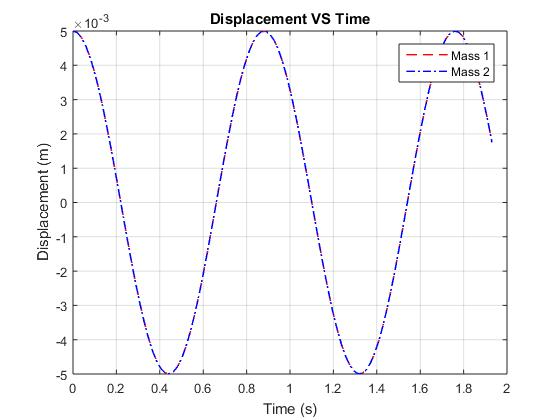
\includegraphics[width=0.7\textwidth]{Figures/R1D.jpg}
		\end{framed}
	\caption{ The displacement of block (mass $m_1$ and mass $m_2$) corresponding to the value from table \ref{tabR1} (case 01).}
	\label{fig:R1}
\end{figure}
 
In this case study 01, equal initial displacement was discussed. As previous stated, in order to analysis this task, initial displacements are 0.005 $m$ both in mass $m_1$ and $m_2$. Figure \ref{fig:R1} depicts the behaviour of displacement over time both masses $m_1$ and $m_2$. Red colour describes the mass 1 ($m_1$) and Blue colour describes the mass 2 ($m_2$). Interestingly, when both masses have same initial displacement which tends to coincide as following figure \ref{fig:R1}. The behaviour of velocity over time both masses $m_1$ and $m_2$ was described in figure \ref{fig:R2}. The velocity curves of the $m_1$ and $m_2$ also tend to coincide with each curve as previous result. 

 \begin{figure}[hbt!]
	\centering
	\begin{framed}
	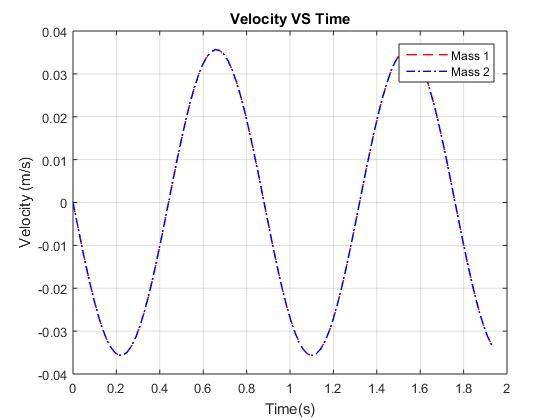
\includegraphics[width=0.7\textwidth]{Figures/R1V.jpg}
		\end{framed}
	\caption{ The velocity of block (mass $m_1$ and mass $m_2$) corresponding to the values from table \ref{tabR1} (case 01).}
	\label{fig:R2}
\end{figure}

\subsection{Case Study 02: Different initial displacement}
\paragraph{}

Now, consider the changing initial conditions and keep the other parameters the same. In this case, only initial displacement of mass 2 ($m_2$) changes into as 0 $m$. Mass 1 ($m_1$) value keeps remain during the process. As earlier used in case 01, in here also initial velocities were kept value as 0 $ms^{-1}$. As a result, figure \ref{fig:R3} was obtained by changing the initial displacement, and this describes the behaviour of the displacement of the $m_1$ and $m_2$. Mass 1 ($m_1$) does have nasty oscillating behaviour during the process, better than mass 2 ($m_2$). Looking at the mass 1 ($m_1$) values, which is less than mass 2 ($m_2$). The smaller amount of $m_1$ displayed a quick, precise behaviour rather than the other mass. When we look at the figure \ref{fig:R4}, the behavior is similar to the behavior discussed in the previous result. The same can be confirmed from the behaviour of mass 1  and mass 2  shown in figure \ref{fig:R4} but it can be observed that they more than oscillated with each other in the previous  velocity described image. Since both masses do not have initial velocities, they both started at zero and ended at the same value. The result we got from this proved to be correct. It can be observed that the eigen frequencies $\omega_1 = 50.9198$ $rads^{-1}$ and $\omega_2 = 264.7758$ $rads^{-1}$ are in this process. Maximum frequency ($f_{max}$) is 2.5898 $Hz$. 



 \begin{figure}[hbt!]
	\centering
	\begin{framed}
	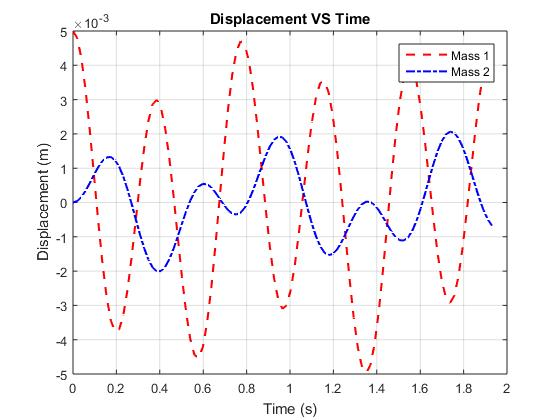
\includegraphics[width=0.7\textwidth]{Figures/R2D.jpg}
	\end{framed}
	\caption{ The displacement of block corresponding to the values from table \ref{tabR1} (case 02). }
	\label{fig:R3}
\end{figure}

\begin{figure}[hbt!]
	\centering
	\begin{framed}
	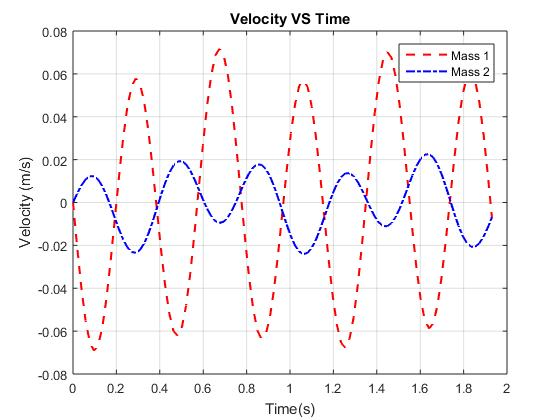
\includegraphics[width=0.7\textwidth]{Figures/R2V.jpg}
		\end{framed}
	\caption{ The velocity of block  corresponding to the values from table \ref{tabR1} (case 02). }
	\label{fig:R4}
\end{figure}

\subsection{Case Study 03: Behavior at the same mass and spring constant values}
\paragraph{}
Now, in order to convert that system into linear system following two method can be implementing. In first case study if
masses having equal initial displacement and, other second case study was change value of $m_2$'s initial displacement. Here, we discuss the interesting case where masses and springs contain the same values.

 \begin{table}[hbt!]
\begin{center}
    \begin{tabular}{p{6cm}|p{2cm}|p{3cm}}
    \hline
    \textbf{Description of constant} & \textbf{Constant} & \textbf{Values}
    \\
    \hline \hline
    Mass 1 & $m_1$ & 0.815 $(kg)$\\
    Mass 1 & $m_1$ & 0.815 $(kg)$\\
    Spring constant 1  & $k_1$ & 41.5 $(N/m)$\\
    Spring constant 2  & $k_2$ & 41.5$(N/m)$\\
    Spring constant 3  & $k_3$ & 41.5 $(N/m)$\\
     Initial position of mass 1 & $x_1$ & 0.005 $(m)$ \\
     Initial position of mass 2 & $x_2$ & 0 $(m)$  \\
     Initial velocity of mass 1 & $\dot{x_1}$ & 0 $m/s$ \\
     Initial velocity of mass 2 & $\dot{x_2}$ & 0 $m/s$  \\
     Time period & $t$ & 100 $(s)$ \\
     \hline
    \end{tabular}
    \caption{Values of the constant corresponding to the case 03. Values were taken from \cite{JETIRRes28:online}. }
    \label{tabR1}
    \end{center}
\end{table}
  
  \begin{figure}[hbt!]
	\centering
	\begin{framed}
	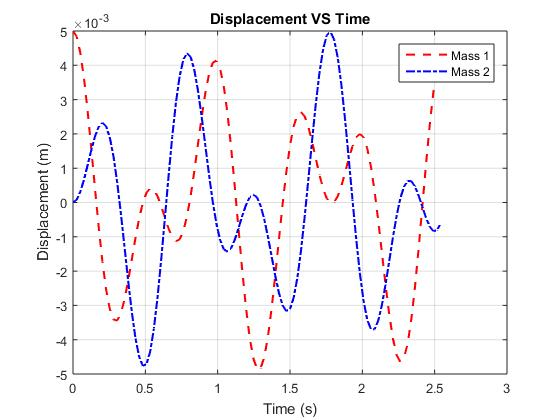
\includegraphics[width=0.7\textwidth]{Figures/R3D.jpg}
		\end{framed}
	\caption{ The displacement of block corresponding to the values from table \ref{tabR1} (case 03). }
	\label{fig:R5}
\end{figure}

  \newpage
  
  
  \begin{figure}[hbt!]
	\centering
	\begin{framed}
	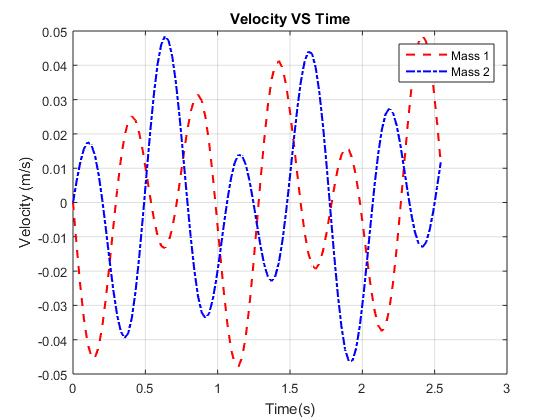
\includegraphics[width=0.7\textwidth]{Figures/R3V.jpg}
		\end{framed}
	\caption{ The velocity of block corresponding to the values from table \ref{tabR1} (case 03). }
	\label{fig:R6}
\end{figure}

When both masses are equal, the obtained expressions are significantly simplified. It can be seen these figure \ref{fig:R5} and figure \ref{fig:R6}. In this case, The mass of the system was set as 0.815 $kg$ in the model.  And the stiffness were set as 41.5 $Nm^{-1}$.  It is interesting to note that the system demonstrates a beating phenomenon, in which energy is transferred cyclically from one mass to the next. It is seen that when the two eigen frequencies are approximately equal. 

\subsection{Summary}
\paragraph{}

 Following table \ref{tbo} explains the details of the each case studies that we have been studied. Looking at the table we realised, the results were obtained by changing a few parameters. 

\begin{table}[h]
\begin{center}
\begin{tabular}{@{}|l|l|l|l|l|l|l|l|l|@{}}
\toprule
Case & $m_1$ $(kg)$ & $m_2$ $(kg)$ & $k_1$ $(N/m)$ & $k_2$ $(N/m)$ & $k_3$ $(N/m)$& $\omega_1$ $(rad/s)$ & $\omega_2$ $(rad/s)$ & $f_{max}$ ($Hz$) \\
\midrule \hline
 1    & 0.815  & 3.099 & 41.5 & 138 & 157.8 & 50.9198 &  264.7758 & 2.5898  \\ 
\hline
2    & 0.815  & 3.099 \footnotemark[1]  & 41.5 & 138 & 157.8 & 50.9198 & 264.7758 & 2.5898 \\ \hline
3    & 0.815  & 0.815  & 41.5 & 41.5 & 41.5 & 50.9202 & 152.7607& 1.9671  \\
\hline
\end{tabular}
\caption{Comparison results}
\label{tbo}
\end{center}
\end{table}

\newpage

\section{Investigate the longitudinal vibrational motion of a (1D) chain}
\paragraph{}
To investigate the dynamics of the vibrational motion in an infinite 1D-chain of identical masses, there are several conditions were considered. To obtain the results, vibration of a linear array of identical atoms corresponding their relevant values will be discussed. In this special case, all the masses are same with its value 0.815 $kg$. And also. in here all the spring constants are same as masses (41.5 $N/m$). The equilibrium separation distance between masses is 0.01 $m$. Using the dispersion relation in above equation discussed in previous section we can calculate their numerical values considering with 100 masses. Following figures will be observed the behaviour of corresponding masses. 


  \begin{figure}[hbt!]
	\centering
	\begin{framed}
	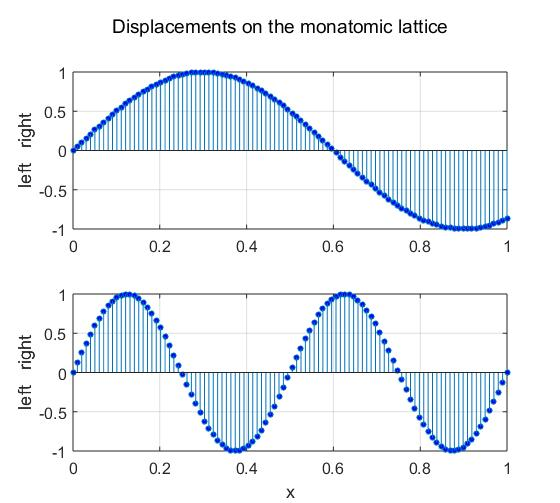
\includegraphics[width=0.8\textwidth]{Figures/N1.jpg}
		\end{framed}
	\caption{ Atomic displacements on the monatomic lattice for a long and short wavelength wave. }
	\label{fig:Lat1}
\end{figure}

Figure \ref{fig:Lat1} shows the results of running the Matlab  with the input parameters: number of masses $n = 100$, separation distance between atoms $d = 0.01$ $m$, mass of each particle $m = 0.815$ $kg$ and spring constant for each spring $k = 10$ $N/m$. In this figure \ref{fig:Lat1} masses displacements on the monatomic lattice for a long and short wavelength wave were displayed. A positive displacement corresponds to a movement to the right and a negative displacement a movement to the left with respect to the equilibrium positions. 

  \begin{figure}[hbt!]
	\centering
	\begin{framed}
	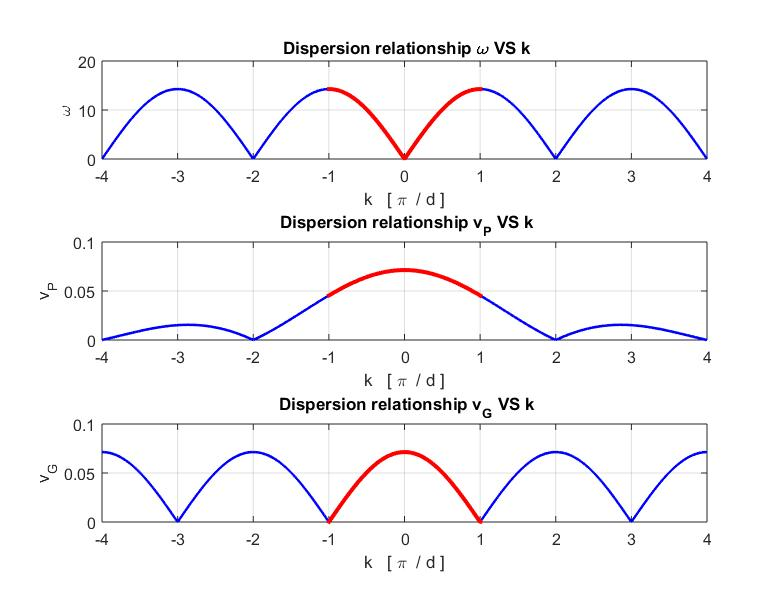
\includegraphics[width=0.9\textwidth]{Figures/N2.jpg}
	\end{framed}
	\caption{ Dispersion relationships for the monatomic lattice. }
	\label{fig:Lat2}
\end{figure}

In this figure \ref{fig:Lat2}, it is seen that particles have been displayed different behaviours due to different conditions. It explains the behaviour of frequency ($\omega$), the behaviour of phase velocity ($V_P$) and the behaviour of group velocity ($V_G$)  with respect to $k_p$. The absolute values must be used, since the frequency is a positive quantity, regardless of whether $k_p$ is positive or negative (which means wave moving to the right or left along the chain). In this process, the maximum angular velocity is $\omega_0$. Above dispersion curve in sub figure 01 clearly shows that for one value of $\omega$ there are several values of wave-vector $k_p$. Therefore we have defined the brillouin zones as first brillouin zone and second brillouin zone. The phase velocity  of a wave is the rate of advance of a point of constant phase along the direction of propagation. In the sub figure 02 explains the phase velocity of the system. A wave is, in general, a superposition of its harmonic components. The ensemble or group of waves is observed to move ahead with a velocity ($d\omega/dt$) known as the group velocity ($V_G$). The group velocity is the velocity with which the wave transmits energy along the propagation direction. No energy can ever be transported past a node in a wave train because the medium at the nodal point is stationary. For the standing waves, the group velocity is zero, and there is zero net energy flow.



\section{Numerical results of two-dimensional spring motion system}
\paragraph{}

This section describes the motion results obtained using Euler's Lagrange equation for a two-dimensional, two-DOF support system comprised of four bilinear springs. The system was obtained by a point mass in a top-view of the four spring mass system, seen in figure \ref{fig:8}. Although, figure \ref{fig:9} depicts the general schematic. As earlier stated, the connector points where one end of every spring connects are considered fixed in space and in line with the two-dimensional plane's $X$ and $Y$ axes. The alignment of the buckles will transform with respect to the original configuration as shown in figure \ref{fig:9} as the mass moves in the two-dimensional plane. These dimensional non linearities will be addressed by calculating the motion's steps at each iteration using Rungre-Kutta fourth order method and updating the equations of motion accordingly. 

\subsection{Case study 01: Behaviour of the mass initial displacement towards the positive $ X $ axis}
\paragraph{}

Case study 01 is defined by the parameters given in
Table 4.1. It is created from the earlier discussed model in section \ref{XY2} and which is only concerned its initial displacement of $X$ axis keeping initial displacement of $Y$ axis zero. 


 \begin{table}[hbt!]
\begin{center}
    \begin{tabular}{p{6cm}|p{2cm}|p{3cm}}
    \hline
    \textbf{Description of constant} & \textbf{Constant} & \textbf{Values}
    \\
    \hline \hline
    Mass of particle  & $m$ & 0.815 $(kg)$\\
      Spring constant of particle  & $k$ & 41.5 $(N/m)$\\
     Initial position of mass $X$ axis & $x$ & 0.005 $(m)$ \\
     Initial position of mass $Y$ axis  & $y$ & 0 $(m)$  \\
     Initial position of mass $X$ axis & $\dot{x}$ & 0 ($m/s$) \\
     Initial position of mass $Y$ axis & $\dot{y}$ & 0 ($m/s$)  \\
     Length of the spring & $l$ & 0.01 ($m$) \\
     Step size & $h$ & 0.01  \\
     Time period & $t$ & 100 $(s)$ \\
     \hline
    \end{tabular}
    \caption{Values of the constant corresponding to the  2D case 01. Mass is moving in $XY$ plane. Several values were taken from \cite{JETIRRes28:online}. }
    \label{tab2D1}
    \end{center}
\end{table}

\newpage 

 \begin{figure}[hbt!]
	\centering
	\begin{framed}
	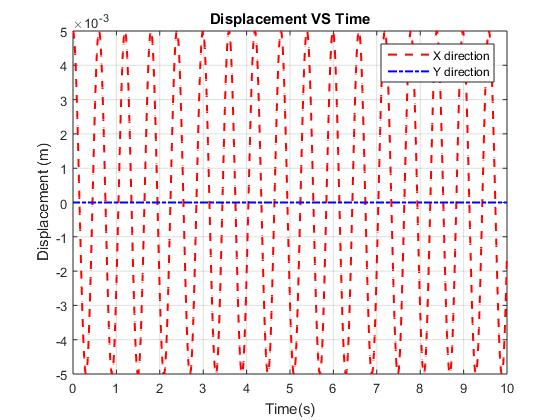
\includegraphics[width=0.66\textwidth]{Figures/2DD.jpg}
		\end{framed}
	\caption{ The displacement of block corresponding to the values from table \ref{tab2D1} (case 01). }
	\label{fig:R5}
\end{figure}

 \begin{figure}[hbt!]
	\centering
	\begin{framed}
	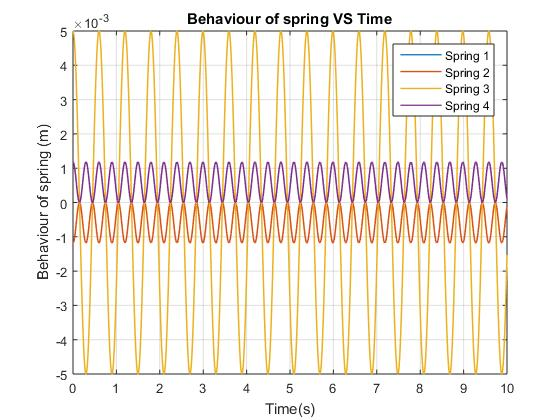
\includegraphics[width=0.66\textwidth]{Figures/2DA.jpg}
	\end{framed}
	\caption{ The displacement of all springs corresponding to the values from table \ref{tab2D1} (case 01). }
	\label{fig:R5}
\end{figure}

 \begin{figure}[hbt!]
	\centering
	\begin{framed}
	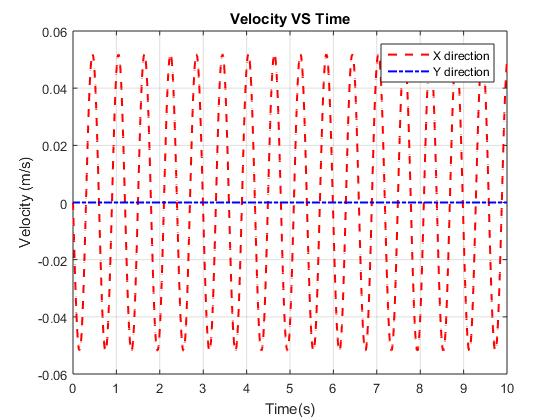
\includegraphics[width=0.7\textwidth]{Figures/2DV.jpg}
		\end{framed}
	\caption{ The velocity of block (mass $m$) corresponding to the values from table \ref{tab2D1} (case 01). }
	\label{fig:R5}
\end{figure}

\newpage

\subsection{Case 02:  Behaviour of the mass initial displacement towards the both positive $X$ and $Y$ axis }
\paragraph{}

In this scenario, Mass has different initial displacements towards both $X$ and $Y$ axis. In the previous case, which has only positive initial displacement  towards $X$  direction. It was set as 0.01 $m$. %To obtain the results, towards $X$ axis displacement and $Y$ axis displacement were assigned as 0.005 $m$ respectively.   

 \begin{table}[hbt!]
\begin{center}
    \begin{tabular}{p{6cm}|p{2cm}|p{3cm}}
    \hline
    \textbf{Description of constant} & \textbf{Constant} & \textbf{Values}
    \\
    \hline \hline
    Mass of particle  & $m$ & 0.815 $(kg)$\\
      Spring constant of particle  & $k$ & 41.5 $(N/m)$\\
     Initial position of mass $X$ axis & $x$ & 0.005 $(m)$ \\
     Initial position of mass $Y$ axis  & $y$ & 0.03 $(m)$  \\
     Initial position of mass $X$ axis & $\dot{x}$ & 0 ($m/s$) \\
     Initial position of mass $Y$ axis & $\dot{y}$ & 0 ($m/s$)  \\
     Length of the spring & $l$ & 0.01 ($m$) \\
     Step size & $h$ & 0.01  \\
     Time period & $t$ & 100 $(s)$ \\
     \hline
    \end{tabular}
    \caption{Values of the constant corresponding to the  2D case 02. Mass is moving in $XY$ plane. Several values were taken from \cite{JETIRRes28:online}. }
    \label{tab2D2}
    \end{center}
\end{table}

\newpage

 \begin{figure}[hbt!]
	\centering
	\begin{framed}
	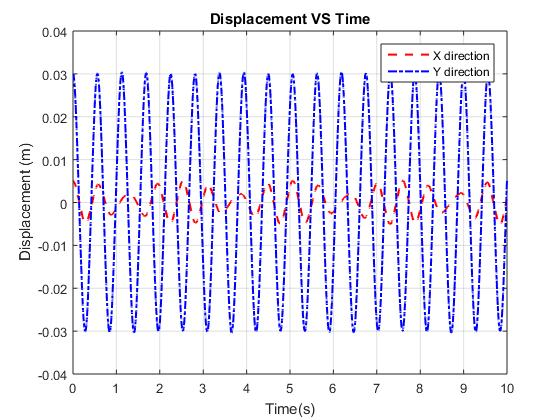
\includegraphics[width=0.66\textwidth]{Figures/2DD2.jpg}
		\end{framed}
	\caption{ The displacement of block corresponding to the values from table \ref{tab2D2} (case 02). }
	\label{fig:221}
\end{figure}

 \begin{figure}[hbt!]
	\centering
	\begin{framed}
	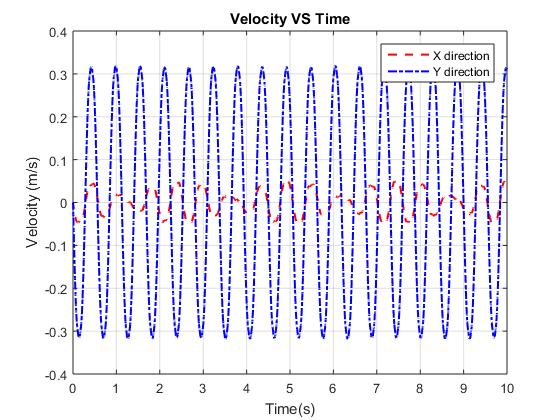
\includegraphics[width=0.66\textwidth]{Figures/2DV2.jpg}
	\end{framed}
	\caption{ The velocity of block corresponding to the values from table \ref{tab2D2} (case 02). }
	\label{fig:222}
\end{figure}

\newpage


 \begin{figure}[hbt!]
	\centering
	\begin{framed}
	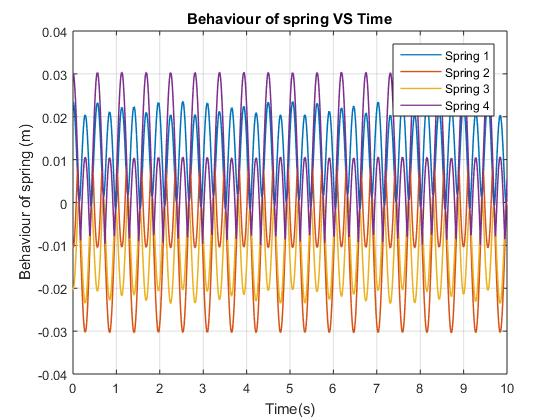
\includegraphics[width=0.7\textwidth]{Figures/2DA2.jpg}
		\end{framed}
	\caption{ The displacement of all springs together corresponding to the values from table \ref{tab2D1} (case 02). }
	\label{fig:223}
\end{figure}

Corresponding to the table \ref{tab2D2} the above results were observed. As shown in figure \ref{fig:221} it can be seen that the displacement of  mass along both $X$ and $Y$ directions. As shown in table  \ref{tab2D2} initial conditions of $x$ and $y$ were defined as 0.005 $m$ and 0.03 $m$ respectively. $y$ has a bigger value than $x$ value. It occurs graphical quality lines corresponding to the given $y$ value. Figure \ref{fig:222} shows the velocity of  mass along both $X$ and $Y$ directions and which depicts the same result that earlier discussed. 

\subsection{Case study 03: Isotropic oscillations 
}
\paragraph{}

In this section, Isotropic oscillations of mass $m$ moving in the two-dimensional will be discussed. To obtain the results, equations \eqref{f1} and \eqref{f2} from section \ref{xo} will be used. In this results phase difference ($\Delta$) will play a major role. The real data of the system are shown in table.  The experimental analysis for the movement of the mass system was done with given values.  

\begin{table}[h]
\begin{center}

\begin{tabular}{@{}|l|l|l|l|l|l|l|l|@{}}
\toprule
 $m$ $(kg)$  & $k$ $(N/m)$ & $l$ $(m)$ & $\omega$ $(rad/s)$& $T (s)$ & $A$ & $B$  & $\Delta$ \\
\midrule \hline
 0.815    & 41.5  & 0.01 & 10.30 & 0.61&  1 &  1& $ 0, \pi/4, \pi/2, 3\pi/4  $  \\ 
\hline
\end{tabular}
\caption{Real data of the system \cite{JETIRRes28:online,levitan1960forced}}
\label{phase1}%
\end{center}
\end{table}

\newpage


 \begin{figure}[hbt!]
	\centering
	\begin{framed}
	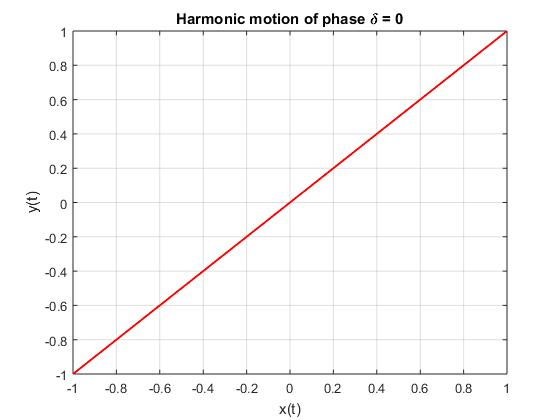
\includegraphics[width=0.68\textwidth]{Figures/0.jpg}
	\end{framed}
	\caption{ Trajectories in a two-dimensional harmonic oscillator potential when $\Delta = 0$. }
	\label{fig:O1}
\end{figure}

 \begin{figure}[hbt!]
	\centering
	\begin{framed}
	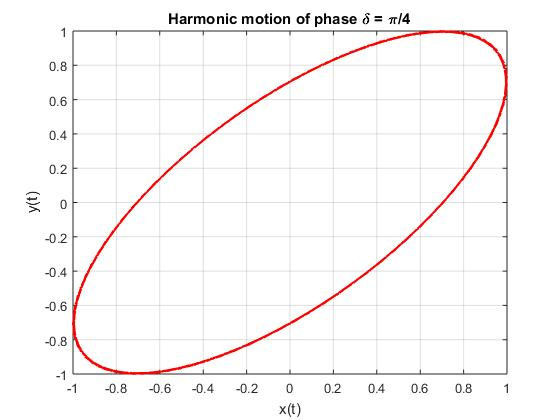
\includegraphics[width=0.68\textwidth]{Figures/p4.jpg}
		\end{framed}
	\caption{ Trajectories in a two-dimensional harmonic oscillator potential when $\Delta = \pi/4 $. }
	\label{fig:O2}
\end{figure}

\newpage

 \begin{figure}[hbt!]
	\centering
	\begin{framed}
	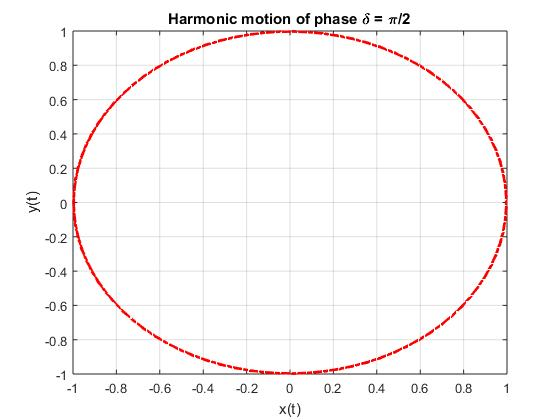
\includegraphics[width=0.68\textwidth]{Figures/p2.jpg}
		\end{framed}
	\caption{ Trajectories in a two-dimensional harmonic oscillator  when $\Delta = \pi/2 $.). }
	\label{fig:03}
\end{figure}


 \begin{figure}[hbt!]
	\centering
	\begin{framed}
	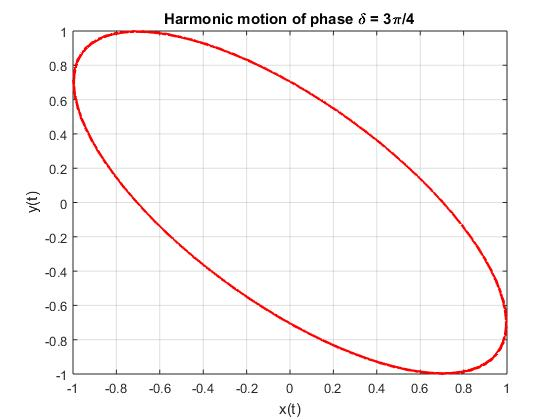
\includegraphics[width=0.68\textwidth]{Figures/3p.jpg}
	\end{framed}
	\caption{ Trajectories in a two-dimensional harmonic oscillator  when $\Delta = 3\pi/4 $. }
	\label{fig:04}
\end{figure}

\newpage

Thus, the combined motion of two simple-harmonics oscillators, one along each axis, with the same angular frequency but differing amplitudes and phase angles, will ensue. The above results prove that they will differ according to their relevant phase difference. Two-dimensional motion of a simple-harmonic oscillator with $A=B=1 m$ and $\Delta= 0$ is shown in figure \ref{fig:O1}. When $\Delta = 0$, the elliptical path of a two-dimensional isotropic oscillator illustrated as shown in figure \ref{fig:O2}. In particular, if the phase difference is equal to $\pi/2$ and $3\pi/4$ in respectively, the results were displayed as shown in figure \ref{fig:03} and  figure \ref{fig:04}. 

\subsection{Case study 04: Anisotropic oscillations}
\paragraph{}
The dynamics of a mass coupled springs are depicted by the  anisotropic oscillator model. In this section, anisotropic oscillations the combined motion of two simple-harmonics oscillators and trajectory map  will be discussed. In this process, both angular frequencies are not same during the process. But other initial conditions keep remain as discussed in table \ref{phase1}. Further, results will be observed two different situations of angular frequencies. The cases can be described as $\omega_x = 2\omega_y$ and $\omega_x = \sqrt{2}\omega_y$.  


 \begin{figure}[hbt!]
	\centering
	\begin{framed}
	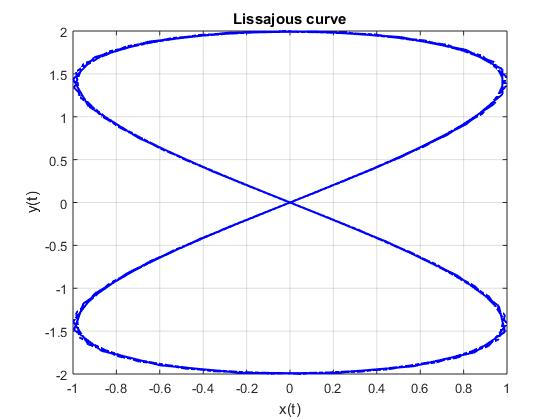
\includegraphics[width=0.7\textwidth]{Figures/Lissajous curve.jpg}
	\end{framed}
	\caption{ Anisotropic oscillations when $\omega_x = 2\omega_y$. }
	\label{fig:O5}
\end{figure}

\newpage

 \begin{figure}[hbt!]
	\centering
	\begin{framed}
	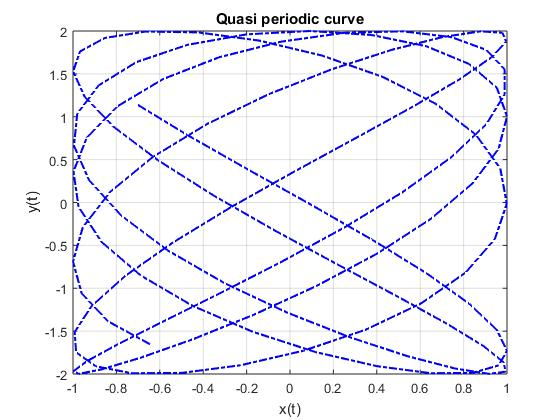
\includegraphics[width=0.7\textwidth]{Figures/quasi periodic.jpg}
	\end{framed}
	\caption{ Quasi periodic curve when $\omega_x = \sqrt{2}\omega_y$. }
	\label{fig:O6}
\end{figure}

The above results were obtained corresponding to the different angular frequencies ($\omega_x \neq \omega_y$). The first result, figure \ref{fig:O5} displayed motion of particle hen $\omega_x = 2\omega_y$. They differ in general, and their ratio determines the mass's orbit in 2-D space. The motion of the mass creates a Lissajous figure is as shown in \ref{fig:O5}.
%\chapter{Results and Discussion}
\label{chap:05}
\paragraph{}

At last, Runge-Kutta fourth order iteration can be used to optimise and enhance the spring mass model's key parameters and performance. The corresponding relationship between the initial conditions and other parameters of the mass can then be determined. As a result, the spring stiffness of mass and other coefficients can be predicted under different conditions, and the dynamic characteristics can be calculated using the numerical method of Runge-Kutta fourth order method. Therefore, the masses dynamic characteristics are precisely estimated during the masses movemnt processes, and the different processes under various given conditions can be described effectively. The numerical results in this section regarding frequency values and outcomes associated with period and other effective parameters yield the following results for the different spring-mass systems presented in the previous section.

\section{Numerical results for the motion of undamped linear spring mass system with coupled two degrees of freedom}
\paragraph{}

In this section, there are three case studies will discussed with analysis results. Results will be interpreted corresponding to the  different parameter values and initial values. As a result, which helps to identify the precise values of parameters during the experiment. 

\subsection{Case Study 01: Equal initial displacement}
\paragraph{}
 In this subsection, equal initial displacement with different mass values and spring stiffness values will be discussed. The following this method can be used to convert that system into a linear system. To obtain the numerical results earlier stated equations will be used. During this process, mass displacement is the same. Which means $x_1$ and $x_2$ have equal values. And also, with this process, initial velocities ($\Dot{x_1}$ and $\Dot{x_2}$) describe neutral moments, which both have zero values. As given table \ref{tabR1} explains the more details about values of the model's parameters.    
\newpage

 \begin{table}[hbt!]
\begin{center}
    \begin{tabular}{p{6cm}|p{2cm}|p{3cm}}
    \hline
    \textbf{Description of constant} & \textbf{Constant} & \textbf{Values}
    \\
    \hline \hline
    Mass 1 & $m_1$ & 0.815 $(kg)$\\
    Mass 1 & $m_1$ & 3.099 $(kg)$\\
      Spring constant 1  & $k_1$ & 41.5 $(N/m)$\\
      Spring constant 2  & $k_2$  &138 $(N/m)$\\
    Spring constant 3  & $k_3$ & 157.8 $(N/m)$\\
     Initial position of mass 1 & $x_1$ & 0.005 $(m)$ \\
     Initial position of mass 2 & $x_2$ & 0.005 $(m)$  \\
     Initial velocity of mass 1 & $\dot{x_1}$ & 0 $m/s$ \\
     Initial velocity of mass 2 & $\dot{x_2}$ & 0 $m/s$  \\
     Step size & $h$ & 0.1  \\
     Time period & $t$ & 100 $(s)$ \\
     \hline
    \end{tabular}
    \caption{Values of the constant corresponding to the case 01. Values were taken from \cite{JETIRRes28:online}. }
    \label{tabR1}
    \end{center}
\end{table}
  

 \begin{figure}[hbt!]
	\centering
	\begin{framed}
	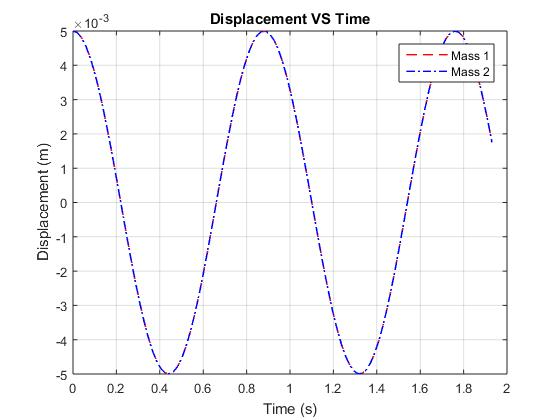
\includegraphics[width=0.7\textwidth]{Figures/R1D.jpg}
		\end{framed}
	\caption{ The displacement of block (mass $m_1$ and mass $m_2$) corresponding to the value from table \ref{tabR1} (case 01).}
	\label{fig:R1}
\end{figure}
 
In this case study 01, equal initial displacement was discussed. As previous stated, in order to analysis this task, initial displacements are 0.005 $m$ both in mass $m_1$ and $m_2$. Figure \ref{fig:R1} depicts the behaviour of displacement over time both masses $m_1$ and $m_2$. Red colour describes the mass 1 ($m_1$) and Blue colour describes the mass 2 ($m_2$). Interestingly, when both masses have same initial displacement which tends to coincide as following figure \ref{fig:R1}. The behaviour of velocity over time both masses $m_1$ and $m_2$ was described in figure \ref{fig:R2}. The velocity curves of the $m_1$ and $m_2$ also tend to coincide with each curve as previous result. 

 \begin{figure}[hbt!]
	\centering
	\begin{framed}
	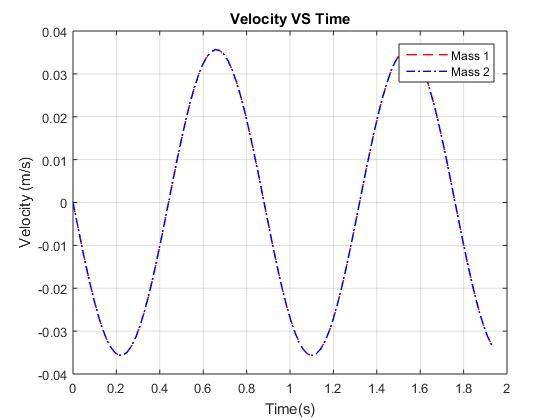
\includegraphics[width=0.7\textwidth]{Figures/R1V.jpg}
		\end{framed}
	\caption{ The velocity of block (mass $m_1$ and mass $m_2$) corresponding to the values from table \ref{tabR1} (case 01).}
	\label{fig:R2}
\end{figure}

\subsection{Case Study 02: Different initial displacement}
\paragraph{}

Now, consider the changing initial conditions and keep the other parameters the same. In this case, only initial displacement of mass 2 ($m_2$) changes into as 0 $m$. Mass 1 ($m_1$) value keeps remain during the process. As earlier used in case 01, in here also initial velocities were kept value as 0 $ms^{-1}$. As a result, figure \ref{fig:R3} was obtained by changing the initial displacement, and this describes the behaviour of the displacement of the $m_1$ and $m_2$. Mass 1 ($m_1$) does have nasty oscillating behaviour during the process, better than mass 2 ($m_2$). Looking at the mass 1 ($m_1$) values, which is less than mass 2 ($m_2$). The smaller amount of $m_1$ displayed a quick, precise behaviour rather than the other mass. When we look at the figure \ref{fig:R4}, the behavior is similar to the behavior discussed in the previous result. The same can be confirmed from the behaviour of mass 1  and mass 2  shown in figure \ref{fig:R4} but it can be observed that they more than oscillated with each other in the previous  velocity described image. Since both masses do not have initial velocities, they both started at zero and ended at the same value. The result we got from this proved to be correct. It can be observed that the eigen frequencies $\omega_1 = 50.9198$ $rads^{-1}$ and $\omega_2 = 264.7758$ $rads^{-1}$ are in this process. Maximum frequency ($f_{max}$) is 2.5898 $Hz$. 



 \begin{figure}[hbt!]
	\centering
	\begin{framed}
	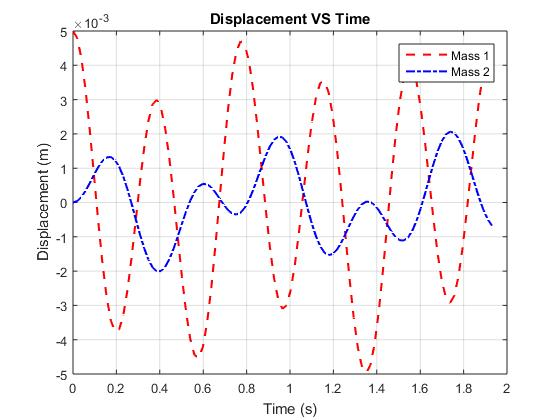
\includegraphics[width=0.7\textwidth]{Figures/R2D.jpg}
	\end{framed}
	\caption{ The displacement of block corresponding to the values from table \ref{tabR1} (case 02). }
	\label{fig:R3}
\end{figure}

\begin{figure}[hbt!]
	\centering
	\begin{framed}
	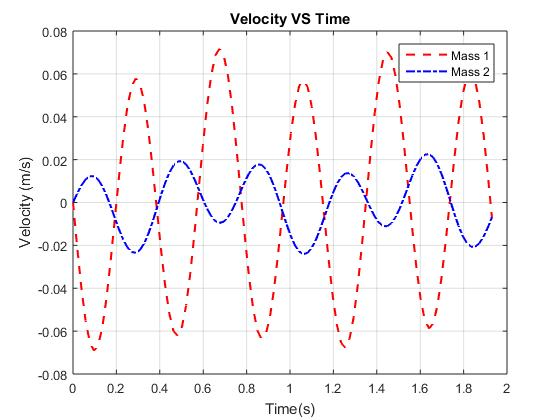
\includegraphics[width=0.7\textwidth]{Figures/R2V.jpg}
		\end{framed}
	\caption{ The velocity of block  corresponding to the values from table \ref{tabR1} (case 02). }
	\label{fig:R4}
\end{figure}

\subsection{Case Study 03: Behavior at the same mass and spring constant values}
\paragraph{}
Now, in order to convert that system into linear system following two method can be implementing. In first case study if
masses having equal initial displacement and, other second case study was change value of $m_2$'s initial displacement. Here, we discuss the interesting case where masses and springs contain the same values.

 \begin{table}[hbt!]
\begin{center}
    \begin{tabular}{p{6cm}|p{2cm}|p{3cm}}
    \hline
    \textbf{Description of constant} & \textbf{Constant} & \textbf{Values}
    \\
    \hline \hline
    Mass 1 & $m_1$ & 0.815 $(kg)$\\
    Mass 1 & $m_1$ & 0.815 $(kg)$\\
    Spring constant 1  & $k_1$ & 41.5 $(N/m)$\\
    Spring constant 2  & $k_2$ & 41.5$(N/m)$\\
    Spring constant 3  & $k_3$ & 41.5 $(N/m)$\\
     Initial position of mass 1 & $x_1$ & 0.005 $(m)$ \\
     Initial position of mass 2 & $x_2$ & 0 $(m)$  \\
     Initial velocity of mass 1 & $\dot{x_1}$ & 0 $m/s$ \\
     Initial velocity of mass 2 & $\dot{x_2}$ & 0 $m/s$  \\
     Time period & $t$ & 100 $(s)$ \\
     \hline
    \end{tabular}
    \caption{Values of the constant corresponding to the case 03. Values were taken from \cite{JETIRRes28:online}. }
    \label{tabR1}
    \end{center}
\end{table}
  
  \begin{figure}[hbt!]
	\centering
	\begin{framed}
	\includegraphics[width=0.7\textwidth]{Figures/R3D.jpg}
		\end{framed}
	\caption{ The displacement of block corresponding to the values from table \ref{tabR1} (case 03). }
	\label{fig:R5}
\end{figure}

  \newpage
  
  
  \begin{figure}[hbt!]
	\centering
	\begin{framed}
	\includegraphics[width=0.7\textwidth]{Figures/R3V.jpg}
		\end{framed}
	\caption{ The velocity of block corresponding to the values from table \ref{tabR1} (case 03). }
	\label{fig:R6}
\end{figure}

When both masses are equal, the obtained expressions are significantly simplified. It can be seen these figure \ref{fig:R5} and figure \ref{fig:R6}. In this case, The mass of the system was set as 0.815 $kg$ in the model.  And the stiffness were set as 41.5 $Nm^{-1}$.  It is interesting to note that the system demonstrates a beating phenomenon, in which energy is transferred cyclically from one mass to the next. It is seen that when the two eigen frequencies are approximately equal. 

\subsection{Summary}
\paragraph{}

 Following table \ref{tbo} explains the details of the each case studies that we have been studied. Looking at the table we realised, the results were obtained by changing a few parameters. 

\begin{table}[h]
\begin{center}
\begin{tabular}{@{}|l|l|l|l|l|l|l|l|l|@{}}
\toprule
Case & $m_1$ $(kg)$ & $m_2$ $(kg)$ & $k_1$ $(N/m)$ & $k_2$ $(N/m)$ & $k_3$ $(N/m)$& $\omega_1$ $(rad/s)$ & $\omega_2$ $(rad/s)$ & $f_{max}$ ($Hz$) \\
\midrule \hline
 1    & 0.815  & 3.099 & 41.5 & 138 & 157.8 & 50.9198 &  264.7758 & 2.5898  \\ 
\hline
2    & 0.815  & 3.099 \footnotemark[1]  & 41.5 & 138 & 157.8 & 50.9198 & 264.7758 & 2.5898 \\ \hline
3    & 0.815  & 0.815  & 41.5 & 41.5 & 41.5 & 50.9202 & 152.7607& 1.9671  \\
\hline
\end{tabular}
\caption{Comparison results}
\label{tbo}
\end{center}
\end{table}

\newpage

\section{Investigate the longitudinal vibrational motion of a (1D) chain}
\paragraph{}
To investigate the dynamics of the vibrational motion in an infinite 1D-chain of identical masses, there are several conditions were considered. To obtain the results, vibration of a linear array of identical atoms corresponding their relevant values will be discussed. In this special case, all the masses are same with its value 0.815 $kg$. And also. in here all the spring constants are same as masses (41.5 $N/m$). The equilibrium separation distance between masses is 0.01 $m$. Using the dispersion relation in above equation discussed in previous section we can calculate their numerical values considering with 100 masses. Following figures will be observed the behaviour of corresponding masses. 


  \begin{figure}[hbt!]
	\centering
	\begin{framed}
	\includegraphics[width=0.8\textwidth]{Figures/N1.jpg}
		\end{framed}
	\caption{ Atomic displacements on the monatomic lattice for a long and short wavelength wave. }
	\label{fig:Lat1}
\end{figure}

Figure \ref{fig:Lat1} shows the results of running the Matlab  with the input parameters: number of masses $n = 100$, separation distance between atoms $d = 0.01$ $m$, mass of each particle $m = 0.815$ $kg$ and spring constant for each spring $k = 10$ $N/m$. In this figure \ref{fig:Lat1} masses displacements on the monatomic lattice for a long and short wavelength wave were displayed. A positive displacement corresponds to a movement to the right and a negative displacement a movement to the left with respect to the equilibrium positions. 

  \begin{figure}[hbt!]
	\centering
	\begin{framed}
	\includegraphics[width=0.9\textwidth]{Figures/N2.jpg}
	\end{framed}
	\caption{ Dispersion relationships for the monatomic lattice. }
	\label{fig:Lat2}
\end{figure}

In this figure \ref{fig:Lat2}, it is seen that particles have been displayed different behaviours due to different conditions. It explains the behaviour of frequency ($\omega$), the behaviour of phase velocity ($V_P$) and the behaviour of group velocity ($V_G$)  with respect to $k_p$. The absolute values must be used, since the frequency is a positive quantity, regardless of whether $k_p$ is positive or negative (which means wave moving to the right or left along the chain). In this process, the maximum angular velocity is $\omega_0$. Above dispersion curve in sub figure 01 clearly shows that for one value of $\omega$ there are several values of wave-vector $k_p$. Therefore we have defined the brillouin zones as first brillouin zone and second brillouin zone. The phase velocity  of a wave is the rate of advance of a point of constant phase along the direction of propagation. In the sub figure 02 explains the phase velocity of the system. A wave is, in general, a superposition of its harmonic components. The ensemble or group of waves is observed to move ahead with a velocity ($d\omega/dt$) known as the group velocity ($V_G$). The group velocity is the velocity with which the wave transmits energy along the propagation direction. No energy can ever be transported past a node in a wave train because the medium at the nodal point is stationary. For the standing waves, the group velocity is zero, and there is zero net energy flow.



\section{Numerical results of two-dimensional spring motion system}
\paragraph{}

This section describes the motion results obtained using Euler's Lagrange equation for a two-dimensional, two-DOF support system comprised of four bilinear springs. The system was obtained by a point mass in a top-view of the four spring mass system, seen in figure \ref{fig:8}. Although, figure \ref{fig:9} depicts the general schematic. As earlier stated, the connector points where one end of every spring connects are considered fixed in space and in line with the two-dimensional plane's $X$ and $Y$ axes. The alignment of the buckles will transform with respect to the original configuration as shown in figure \ref{fig:9} as the mass moves in the two-dimensional plane. These dimensional non linearities will be addressed by calculating the motion's steps at each iteration using Rungre-Kutta fourth order method and updating the equations of motion accordingly. 

\subsection{Case study 01: Behaviour of the mass initial displacement towards the positive $ X $ axis}
\paragraph{}

Case study 01 is defined by the parameters given in
Table 4.1. It is created from the earlier discussed model in section \ref{XY2} and which is only concerned its initial displacement of $X$ axis keeping initial displacement of $Y$ axis zero. 


 \begin{table}[hbt!]
\begin{center}
    \begin{tabular}{p{6cm}|p{2cm}|p{3cm}}
    \hline
    \textbf{Description of constant} & \textbf{Constant} & \textbf{Values}
    \\
    \hline \hline
    Mass of particle  & $m$ & 0.815 $(kg)$\\
      Spring constant of particle  & $k$ & 41.5 $(N/m)$\\
     Initial position of mass $X$ axis & $x$ & 0.005 $(m)$ \\
     Initial position of mass $Y$ axis  & $y$ & 0 $(m)$  \\
     Initial position of mass $X$ axis & $\dot{x}$ & 0 ($m/s$) \\
     Initial position of mass $Y$ axis & $\dot{y}$ & 0 ($m/s$)  \\
     Length of the spring & $l$ & 0.01 ($m$) \\
     Step size & $h$ & 0.01  \\
     Time period & $t$ & 100 $(s)$ \\
     \hline
    \end{tabular}
    \caption{Values of the constant corresponding to the  2D case 01. Mass is moving in $XY$ plane. Several values were taken from \cite{JETIRRes28:online}. }
    \label{tab2D1}
    \end{center}
\end{table}

\newpage 

 \begin{figure}[hbt!]
	\centering
	\begin{framed}
	\includegraphics[width=0.66\textwidth]{Figures/2DD.jpg}
		\end{framed}
	\caption{ The displacement of block corresponding to the values from table \ref{tab2D1} (case 01). }
	\label{fig:R5}
\end{figure}

 \begin{figure}[hbt!]
	\centering
	\begin{framed}
	\includegraphics[width=0.66\textwidth]{Figures/2DA.jpg}
	\end{framed}
	\caption{ The displacement of all springs corresponding to the values from table \ref{tab2D1} (case 01). }
	\label{fig:R5}
\end{figure}

 \begin{figure}[hbt!]
	\centering
	\begin{framed}
	\includegraphics[width=0.7\textwidth]{Figures/2DV.jpg}
		\end{framed}
	\caption{ The velocity of block (mass $m$) corresponding to the values from table \ref{tab2D1} (case 01). }
	\label{fig:R5}
\end{figure}

\newpage

\subsection{Case 02:  Behaviour of the mass initial displacement towards the both positive $X$ and $Y$ axis }
\paragraph{}

In this scenario, Mass has different initial displacements towards both $X$ and $Y$ axis. In the previous case, which has only positive initial displacement  towards $X$  direction. It was set as 0.01 $m$. %To obtain the results, towards $X$ axis displacement and $Y$ axis displacement were assigned as 0.005 $m$ respectively.   

 \begin{table}[hbt!]
\begin{center}
    \begin{tabular}{p{6cm}|p{2cm}|p{3cm}}
    \hline
    \textbf{Description of constant} & \textbf{Constant} & \textbf{Values}
    \\
    \hline \hline
    Mass of particle  & $m$ & 0.815 $(kg)$\\
      Spring constant of particle  & $k$ & 41.5 $(N/m)$\\
     Initial position of mass $X$ axis & $x$ & 0.005 $(m)$ \\
     Initial position of mass $Y$ axis  & $y$ & 0.03 $(m)$  \\
     Initial position of mass $X$ axis & $\dot{x}$ & 0 ($m/s$) \\
     Initial position of mass $Y$ axis & $\dot{y}$ & 0 ($m/s$)  \\
     Length of the spring & $l$ & 0.01 ($m$) \\
     Step size & $h$ & 0.01  \\
     Time period & $t$ & 100 $(s)$ \\
     \hline
    \end{tabular}
    \caption{Values of the constant corresponding to the  2D case 02. Mass is moving in $XY$ plane. Several values were taken from \cite{JETIRRes28:online}. }
    \label{tab2D2}
    \end{center}
\end{table}

\newpage

 \begin{figure}[hbt!]
	\centering
	\begin{framed}
	\includegraphics[width=0.66\textwidth]{Figures/2DD2.jpg}
		\end{framed}
	\caption{ The displacement of block corresponding to the values from table \ref{tab2D2} (case 02). }
	\label{fig:221}
\end{figure}

 \begin{figure}[hbt!]
	\centering
	\begin{framed}
	\includegraphics[width=0.66\textwidth]{Figures/2DV2.jpg}
	\end{framed}
	\caption{ The velocity of block corresponding to the values from table \ref{tab2D2} (case 02). }
	\label{fig:222}
\end{figure}

\newpage


 \begin{figure}[hbt!]
	\centering
	\begin{framed}
	\includegraphics[width=0.7\textwidth]{Figures/2DA2.jpg}
		\end{framed}
	\caption{ The displacement of all springs together corresponding to the values from table \ref{tab2D1} (case 02). }
	\label{fig:223}
\end{figure}

Corresponding to the table \ref{tab2D2} the above results were observed. As shown in figure \ref{fig:221} it can be seen that the displacement of  mass along both $X$ and $Y$ directions. As shown in table  \ref{tab2D2} initial conditions of $x$ and $y$ were defined as 0.005 $m$ and 0.03 $m$ respectively. $y$ has a bigger value than $x$ value. It occurs graphical quality lines corresponding to the given $y$ value. Figure \ref{fig:222} shows the velocity of  mass along both $X$ and $Y$ directions and which depicts the same result that earlier discussed. 

\subsection{Case study 03: Isotropic oscillations 
}
\paragraph{}

In this section, Isotropic oscillations of mass $m$ moving in the two-dimensional will be discussed. To obtain the results, equations \eqref{f1} and \eqref{f2} from section \ref{xo} will be used. In this results phase difference ($\Delta$) will play a major role. The real data of the system are shown in table.  The experimental analysis for the movement of the mass system was done with given values.  

\begin{table}[h]
\begin{center}

\begin{tabular}{@{}|l|l|l|l|l|l|l|l|@{}}
\toprule
 $m$ $(kg)$  & $k$ $(N/m)$ & $l$ $(m)$ & $\omega$ $(rad/s)$& $T (s)$ & $A$ & $B$  & $\Delta$ \\
\midrule \hline
 0.815    & 41.5  & 0.01 & 10.30 & 0.61&  1 &  1& $ 0, \pi/4, \pi/2, 3\pi/4  $  \\ 
\hline
\end{tabular}
\caption{Real data of the system \cite{JETIRRes28:online,levitan1960forced}}
\label{phase1}%
\end{center}
\end{table}

\newpage


 \begin{figure}[hbt!]
	\centering
	\begin{framed}
	\includegraphics[width=0.68\textwidth]{Figures/0.jpg}
	\end{framed}
	\caption{ Trajectories in a two-dimensional harmonic oscillator potential when $\Delta = 0$. }
	\label{fig:O1}
\end{figure}

 \begin{figure}[hbt!]
	\centering
	\begin{framed}
	\includegraphics[width=0.68\textwidth]{Figures/p4.jpg}
		\end{framed}
	\caption{ Trajectories in a two-dimensional harmonic oscillator potential when $\Delta = \pi/4 $. }
	\label{fig:O2}
\end{figure}

\newpage

 \begin{figure}[hbt!]
	\centering
	\begin{framed}
	\includegraphics[width=0.68\textwidth]{Figures/p2.jpg}
		\end{framed}
	\caption{ Trajectories in a two-dimensional harmonic oscillator  when $\Delta = \pi/2 $.). }
	\label{fig:03}
\end{figure}


 \begin{figure}[hbt!]
	\centering
	\begin{framed}
	\includegraphics[width=0.68\textwidth]{Figures/3p.jpg}
	\end{framed}
	\caption{ Trajectories in a two-dimensional harmonic oscillator  when $\Delta = 3\pi/4 $. }
	\label{fig:04}
\end{figure}

\newpage

Thus, the combined motion of two simple-harmonics oscillators, one along each axis, with the same angular frequency but differing amplitudes and phase angles, will ensue. The above results prove that they will differ according to their relevant phase difference. Two-dimensional motion of a simple-harmonic oscillator with $A=B=1 m$ and $\Delta= 0$ is shown in figure \ref{fig:O1}. When $\Delta = 0$, the elliptical path of a two-dimensional isotropic oscillator illustrated as shown in figure \ref{fig:O2}. In particular, if the phase difference is equal to $\pi/2$ and $3\pi/4$ in respectively, the results were displayed as shown in figure \ref{fig:03} and  figure \ref{fig:04}. 

\subsection{Case study 04: Anisotropic oscillations}
\paragraph{}
The dynamics of a mass coupled springs are depicted by the  anisotropic oscillator model. In this section, anisotropic oscillations the combined motion of two simple-harmonics oscillators and trajectory map  will be discussed. In this process, both angular frequencies are not same during the process. But other initial conditions keep remain as discussed in table \ref{phase1}. Further, results will be observed two different situations of angular frequencies. The cases can be described as $\omega_x = 2\omega_y$ and $\omega_x = \sqrt{2}\omega_y$.  


 \begin{figure}[hbt!]
	\centering
	\begin{framed}
	\includegraphics[width=0.7\textwidth]{Figures/Lissajous curve.jpg}
	\end{framed}
	\caption{ Anisotropic oscillations when $\omega_x = 2\omega_y$. }
	\label{fig:O5}
\end{figure}

\newpage

 \begin{figure}[hbt!]
	\centering
	\begin{framed}
	\includegraphics[width=0.7\textwidth]{Figures/quasi periodic.jpg}
	\end{framed}
	\caption{ Quasi periodic curve when $\omega_x = \sqrt{2}\omega_y$. }
	\label{fig:O6}
\end{figure}

The above results were obtained corresponding to the different angular frequencies ($\omega_x \neq \omega_y$). The first result, figure \ref{fig:O5} displayed motion of particle hen $\omega_x = 2\omega_y$. They differ in general, and their ratio determines the mass's orbit in 2-D space. The motion of the mass creates a Lissajous figure is as shown in \ref{fig:O5}.
\chapter{Conclusion}
\label{chap:06}

\paragraph{}

The goal of this project is to provide insight for the design of coupled one dimensions (1D) and two dimensions (2D) spring mass models. During the project, the motion of the coupled oscillator systems (both 1D and 2D) has been studied  and observed numerically using the Runge Kutta Fourth order method. Throughout the project, there are three objectives have been considered. Investigate the motion for undamped linear spring mass systems with coupled two degrees of freedom, investigate the motion for undamped linear spring mass systems with coupled many degrees of freedom and investigate the two-dimensional spring motion: the mass m is free to move in the XY plane were discussed graphically and numerically.

First, the motion for undamped linear spring systems with coupled two degrees of freedom was analyzed to provide insight for the its numerical behaviour. In this case, analytical formulas for the approximate eigenvectors and eigenvalues were developed. The changing the parameters values (mass of particle, initial displacement and etc )
procedure which makes it relatively simple to perform based on the approximate eigenvalues and eigenvectors. Although, different behaviours. In this case there are three cases were discussed. First, started all the two masses and spring constant are different with each other. But their initial displacements are 0.005 $m$ both $m_1$ and $m_2$ masses respectively. After the system was released, the displacement and speed of the system corresponded to each other. That because which has same initial displacements. After that, the initial displacements of different values were different from each other and the other parameters remained constant. It could be seen that the anti symmetrical behaviour of the figures. Finally, changed the only initial displacement of $x_1$ was changed while $x_2$ was zero.  Other parameters are kept constant. It is interesting to note that
the system demonstrates a beating phenomenon, in which energy is transferred cyclically from one mass to the next. When the two eigen frequencies are approximately equal, this common behaviour basically happens. Interestingly, it could be seen that  mass ratio ($\mu = \frac{m_2}{m_1}$) should be $\mu$ $\geq$ 0 if there is no energy leakage. 

Then, the motion for undamped linear spring mass systems with coupled many degrees of freedom was observed. In this case, the application of dynamics of one dimensional (1D) infinite monoatomic chain of atoms were  yielded with different conditions. In this scenario, frequency ($\omega$), phase velocity ($V_P$) and group velocity ($V_G$) played a major throughout the experiment. In the reuslts, dispersion curve clearly shows that for one value of $\omega$ there are several values of wave-vector $K_p$.  

When discussing simple-harmonic motion in two dimensional, the motion can always be divided into two components, each directed along one of the two coordinate axes ($X$ and $Y$ axes). Lastly, two dimensional sprig mass model was explained with figures. There are four case studies (case study 01. case study 01, case study 03 and case study 04) were discussed considering 2D motion the connector points where one end of every spring connects are considered fixed in space and in line with the two-dimensional plane’s $X$ and$Y$ axes. Case study 01 reveled numerical results which included only the mass initial displacement towards the positive $X$ axis. It can be seen that system oscillates $X$ component (displacement and velocity) if there is an initial displacement towards the positive $X$ axis. In the case study 02, If both initial displacement defined with value it can be seen that the displacement and velocity of mass along both $X$ and $Y$ directions. Behaviour of particle depends on the input initial value. Case study 03, isotropic oscillations of mass $m$ moving in the two-dimensional will be discussed. The results of case study 03 have been proved  that they will differ according to their relevant phase difference $\Delta$. Corresponding phase difference are  $\Delta = 0 $, $\Delta = \pi/4 $ , $\Delta = \pi/2 $ and $\Delta = 3\pi/4 $. Note that when ${\mit\Delta}=0$ the trajectory generates into a straight-line  and for the phase difference values it can be seen that system has an ellipse. Concluded, the easiest way to examine this type of motion is by actually looking at figures of derived, the trajectory carried out by the particle. Looking at the case study 04, the dynamics of a mass coupled springs are depicted by the anisotropic oscillator model. In this process, the angular frequency of the motion along the $X$ axis may be different from the angular frequency of the motion along the $y$ axis.  But other initial conditions keep remain as discussed in earlier. The trajectory described by the particle is called a Lissajous curve when $\omega_x = 2\omega_y$. Although when $\omega_x = \sqrt{2}\omega_y$ output trajectory described by the particle is called a quasi periodic. 

Many engineering problems are modelled and solved using mass-spring systems as the physical foundation. Such models are utilised in the construction of architectural structures or, for example, in the development of sportswear, among other things in modern life. Of fact, in real life, the system of equations of spring masses can be far more complex.
%\chapter{Conclusion}
\label{chap:06}

\paragraph{}

The goal of this project is to provide insight for the design of coupled one dimensions (1D) and two dimensions (2D) spring mass models. During the project, the motion of the coupled oscillator systems (both 1D and 2D) has been studied  and observed numerically using the Runge Kutta Fourth order method. Throughout the project, there are three objectives have been considered. Investigate the motion for undamped linear spring mass systems with coupled two degrees of freedom, investigate the motion for undamped linear spring mass systems with coupled many degrees of freedom and investigate the two-dimensional spring motion: the mass m is free to move in the XY plane were discussed graphically and numerically.

First, the motion for undamped linear spring systems with coupled two degrees of freedom was analyzed to provide insight for the its numerical behaviour. In this case, analytical formulas for the approximate eigenvectors and eigenvalues were developed. The changing the parameters values (mass of particle, initial displacement and etc )
procedure which makes it relatively simple to perform based on the approximate eigenvalues and eigenvectors. Although, different behaviours. In this case there are three cases were discussed. First, started all the two masses and spring constant are different with each other. But their initial displacements are 0.005 $m$ both $m_1$ and $m_2$ masses respectively. After the system was released, the displacement and speed of the system corresponded to each other. That because which has same initial displacements. After that, the initial displacements of different values were different from each other and the other parameters remained constant. It could be seen that the anti symmetrical behaviour of the figures. Finally, changed the only initial displacement of $x_1$ was changed while $x_2$ was zero.  Other parameters are kept constant. It is interesting to note that
the system demonstrates a beating phenomenon, in which energy is transferred cyclically from one mass to the next. When the two eigen frequencies are approximately equal, this common behaviour basically happens. Interestingly, it could be seen that  mass ratio ($\mu = \frac{m_2}{m_1}$) should be $\mu$ $\geq$ 0 if there is no energy leakage. 

Then, the motion for undamped linear spring mass systems with coupled many degrees of freedom was observed. In this case, the application of dynamics of one dimensional (1D) infinite monoatomic chain of atoms were  yielded with different conditions. In this scenario, frequency ($\omega$), phase velocity ($V_P$) and group velocity ($V_G$) played a major throughout the experiment. In the reuslts, dispersion curve clearly shows that for one value of $\omega$ there are several values of wave-vector $K_p$.  

When discussing simple-harmonic motion in two dimensional, the motion can always be divided into two components, each directed along one of the two coordinate axes ($X$ and $Y$ axes). Lastly, two dimensional sprig mass model was explained with figures. There are four case studies (case study 01. case study 01, case study 03 and case study 04) were discussed considering 2D motion the connector points where one end of every spring connects are considered fixed in space and in line with the two-dimensional plane’s $X$ and$Y$ axes. Case study 01 reveled numerical results which included only the mass initial displacement towards the positive $X$ axis. It can be seen that system oscillates $X$ component (displacement and velocity) if there is an initial displacement towards the positive $X$ axis. In the case study 02, If both initial displacement defined with value it can be seen that the displacement and velocity of mass along both $X$ and $Y$ directions. Behaviour of particle depends on the input initial value. Case study 03, isotropic oscillations of mass $m$ moving in the two-dimensional will be discussed. The results of case study 03 have been proved  that they will differ according to their relevant phase difference $\Delta$. Corresponding phase difference are  $\Delta = 0 $, $\Delta = \pi/4 $ , $\Delta = \pi/2 $ and $\Delta = 3\pi/4 $. Note that when ${\mit\Delta}=0$ the trajectory generates into a straight-line  and for the phase difference values it can be seen that system has an ellipse. Concluded, the easiest way to examine this type of motion is by actually looking at figures of derived, the trajectory carried out by the particle. Looking at the case study 04, the dynamics of a mass coupled springs are depicted by the anisotropic oscillator model. In this process, the angular frequency of the motion along the $X$ axis may be different from the angular frequency of the motion along the $y$ axis.  But other initial conditions keep remain as discussed in earlier. The trajectory described by the particle is called a Lissajous curve when $\omega_x = 2\omega_y$. Although when $\omega_x = \sqrt{2}\omega_y$ output trajectory described by the particle is called a quasi periodic. 

Many engineering problems are modelled and solved using mass-spring systems as the physical foundation. Such models are utilised in the construction of architectural structures or, for example, in the development of sportswear, among other things in modern life. Of fact, in real life, the system of equations of spring masses can be far more complex.





%%%%%%%%%%%%%%%%%%%%%%%%%%%%%% APPENDIX %%%%%%%%%%%%%%%%%%%%%%%%%%%%%%%%%%%%%%%%%%%%%%%%%%%%%
\begin{appendix}
\chapter*{Appendix}


\textbf{\Large Code 01}\\

\begin{framed}
\begin{verbatim}
    clc;
clear all;

%Degree of freedom


%input mass_1
M1 = 0.815
%input mass_2
M2 = 3.099

%Inputs for spring constants.
K1 = 41.5

%Inputs for spring constants.
K2 = 138

%Inputs for spring constants.
K3 = 157.8

%Mass matrix
M = [M1 0; 0 M2];

%Stiffness matrix
K = [K1+K2 -K2 ; -K2 K2+K3];

%Estimation natural frequncies and mode shapes

[modeShape fr] = eig(K,M);

%Coffecient matrix

A00 = zeros(2);
A11 = eye(2);
CC = [A00 A11; -inv(M)*K A00];
global CC

%%Time step and time vector

max_freq = max(sqrt(diag(fr))/(2*pi)); %maximum frequency in Hz
dt = 1/(max_freq*20);
Nstep = 100;
time = 0:dt:Nstep*dt;

y0 = [0.005 0.005 0 0]; %[disp1 disp2 vol1 vol2] inatial condition
[tsol,ysol] = ode45('testcode',time,y0);

y1 = ysol(:,1);
y2 = ysol(:,2);
v1 = ysol(:,3);
v2 = ysol(:,4);

idxmin = find(y1 == max(y1))
idxmax = find(y1 == min(y1))



figure()
plot(time,y1,'--r','linewidth',1.5);
hold on
plot(time,y2,'-.b','linewidth',1.5);
hold off
% plot(y1(idxmin),y1(idxmax),'*','MarkerFaceColor','red',...
%     'MarkerSize',10)
% % hold on
% % plot(y2(idxmax),y1(idxmax),'-p','MarkerFaceColor','black',...
% %     'MarkerSize',10)
% hold off
xlabel('Time (s)');
ylabel('Displacement (m)');
title('Displacement VS Time')
legend('Mass 1','Mass 2');
grid on

figure()
plot(time,v1,'--r','linewidth',1.5);
hold on
plot(time,v2,'-.b','linewidth',1.5);
hold on
xlabel('Time(s)');
ylabel('Velocity (m/s)');
title('Velocity VS Time')
legend('Mass 1','Mass 2');
grid on

figure()
plot(y1,y2,'--r','linewidth',1);
hold on
xlabel('Time(s)');
ylabel('Velocity (m/s)');
title('Velocity VS Time')
legend('Mass 1','Mass 2');
grid on


\end{verbatim}
\end{framed}

\newpage

\begin{framed}
\begin{verbatim}
    clear all; 
close all;
clc;
tic

%input mass_1
m1 = input('Enter value of mass_1 (kg):   \n');
%input mass_2
m2 = input('Enter value of mass_2 (kg):   \n');

%Inputs for spring constants.
k1 = input('Enter value of the spring constants (N/m): \n');
%Inputs for spring constants.
k2 = input('Enter value of the spring constants (N/m): \n');
%Inputs for spring constants.
k3 = input('Enter value of the spring constants (N/m): \n');

x10=1; % mass 1 initial position 
x20=1; % mass 2 initial position 

v10=0; % mass 1 initial velocity 
v20=0; % mass 2 initial velocity 

% Set time step 
simTime=1; % simulation time 
tStep=0.01; % simulation time step

iterations=simTime/tStep;
t=0:iterations;

% variables for speed
x1=zeros(iterations,1);
x1(1,:)=x10;
x2=zeros(iterations,1);
x2(1,:)=x20;

v1=zeros(iterations,1);
v1(1,:)=v10;
v2=zeros(iterations,1);
v2(1,:)=v20;

a1=zeros(iterations,1);
a1(1,:)=( k3*(x20-x10) + -k1*x10)/m1;
a2=zeros(iterations,1);
a2(1,:)= (-(k2+k3)*x20 + k3*x10)/m2;

% Set up video
v=VideoWriter('twomass.avi');
v.FrameRate=100;
open(v);

set(gcf, 'Position',  [50, 50, 700, 600])%positions of plot

for n=2:(iterations+1)
    
  %euler method
    
  x1(n,:)=x1(n-1,:)+v1(n-1,:)*tStep;
  x2(n,:)=x2(n-1,:)+v2(n-1,:)*tStep;
  
  v1(n,:)=v1(n-1,:)+a1(n-1,:)*tStep;
  v2(n,:)=v2(n-1,:)+a2(n-1,:)*tStep;
  
  a1(n,:)=(k3*((x2(n,:))-(x1(n,:)))+-k1*(x1(n,:)))/m1;
  a2(n,:)=(-(k2+k3)*(x2(n,:))+k3*(x1(n,:)))/m2;

  % Plot for the video
  subplot(4,1,1)
  
  hold on;
  plot(t(:,1:n),x1(1:n,:),'r')
  plot(t(:,1:n),x2(1:n,:),'m')
  
  xlim([0 iterations])
  ylabel('Position(m)')
  legend('mass 1','mass 2')
  
  subplot(4,1,2)
  
  hold on;
  plot(t(:,1:n),v1(1:n,:),'b')
  plot(t(:,1:n),v2(1:n,:),'c')
 
  xlim([0 iterations])
  ylabel('Velocity(m/s)')
  legend('mass 1','mass 2')
  
  subplot(4,1,3)
  
  hold on;
  plot(t(:,1:n),a1(1:n,:),'g')
  plot(t(:,1:n),a2(1:n,:),'y')
 
  xlim([0 iterations])
  ylabel('Acceleration(m/s^2)')
  legend('mass 1','mass 2')
  
  subplot(4,1,4)
  
  hold on;
  fill([0 9 9 0],[0 0 1.5 1.5],'w'); % clears background
  
  plot([x1(n,:)+3 0],[0.25 0.25],'k'); % springs
  plot([x1(n,:)+3 x2(n,:)+6],[0.25 0.25],'k');
  plot([x2(n,:)+6 9],[0.25 0.25],'k');
  
  fill([x1(n,:)+2.75 x1(n,:)+3.25 x1(n,:)+3.25 x1(n,:)+2.75],
  [0 0 0.5 0.5],'g'); % mass 1
  fill([x2(n,:)+5.75 x2(n,:)+6.25 x2(n,:)+6.25 x2(n,:)+5.75],
  [0 0 0.5 0.5],'g'); % mass 2
  
  fill([0 0.1 0.1 0],[0 0 1 1],[0.5 0.5 0.5]);
  fill([8.9 9 9 8.9],[0 0 1 1],[0.5 0.5 0.5]);

  xlim([0 9]);
  ylim([0 1.5]);
  frame=getframe(gcf);
  writeVideo(v,frame)
  
end
close(v);

figure,

subplot(3,1,1)
hold on;
plot(t',x1,'r')
plot(t',x2,'m')
ylabel('Position (m)')
title('Position, Velocity, & Acceleration as a Function of Time')
legend('mass1','mass2')
grid on

subplot(3,1,2)
hold on;
plot(t',v1,'b')
plot(t',v2,'c')
ylabel('Velocity (m/s)')
legend('mass1','mass2')
grid on

subplot(3,1,3)
hold on;
plot(t',a1,'g')
plot(t',a2,'y')
ylabel('Acceleration (m/s^2)')
xlabel('time (iterations)')
legend('mass1','mass2')
grid on

toc


\end{verbatim}
\end{framed}

\begin{framed}
\begin{verbatim}
    function [x_new,y_new] = sp1(x0,y0,x1,y1,n,r)
x=x0:((x1-x0)/n):x1;
y=((y1-y0)/(x1-x0))*x+y0-((y1-y0)/(x1-x0))*x0;
m=(y1-y0)/(x1-x0);
T=abs(atan(m));
s=length(x);
x_new=zeros(1,s);
y_new=zeros(1,s);
for i=1:s
  x_new(i)=x(i)+r*(-1)^(i)*sin(T);
  y_new(i)=y(i)+r*(-1)^(i)*cos(T);
end
\end{verbatim}
\end{framed}

\newpage

\textbf{\Large Code 02}\\






\begin{framed}
\begin{verbatim}

clear all; 
close all;
clc;

% Assume spring constants are equivalent and masses are equivelent.

%input Mass Value
m = input('Enter value of Mass Weight (kg):   \n');
%Input for spring constants.
k = input('Enter value of the spring constants (N/m): \n');
%Input for spring constants.
n = input('Number of Masses: \n');
% simulation time
t = input('Simulation time period: \n');

tStep=0.001;
mode=2; % must be <= n

% Create mass and stiffness matrices based on generalized FBD's

% mass matrix is an identity matrix
M=m.*eye(n); 
e=ones(n,1);

% stiffness matrix
K=spdiags([-k.*e 2*k.*e -k.*e],-1:1,n,n);

% make the K matrix into a full matrix
K=full(K); 

% Returns phi (eigenvectors) and lambda (eigenvalues) - M*phi*lambda=K*phi
[phi,lambda]=eig(K,M);
% Get natural frequencies from eigenvalues
Wn=sqrt(diag(lambda)); 

% Time step setup
% total number of iterations
iterations=t/tStep;

% time vector (for plotting purposes)
tVector=tStep.*(1:iterations); 

% Pre-allocate arrays for speed
x=zeros(iterations,n);
v=zeros(iterations,n);
a=zeros(iterations,n);

% initial displacements governed by desired mode
x(1,:)=phi(:,mode); 

% Iteratively solve equations of motion using Semi-implicit Euler
for i=2:iterations
    for j=1:n
        a(i,j)=(-K(j,:)./M(j,j))*(x(i-1,:)');
        v(i,j)=v(i-1,j)+a(i,j)*tStep;
        x(i,j)=x(i-1,j)+v(i,j)*tStep;
    end
end

% Plot the results
for k=1:n
    subplot(3,1,1); hold on; grid on;
    plot(tVector,x(:,k))
    subplot(3,1,2); hold on; grid on;
    plot(tVector,v(:,k))
    subplot(3,1,3); hold on; grid on;
    plot(tVector,a(:,k))
end

subplot(3,1,1);
title('Position, Velocity, and Acceleration as a Function of Time');
ylabel('Position (m)');
grid on;

subplot(3,1,2);
ylabel('Velocity (m/s)');
subplot(3,1,3);
ylabel('Acceleration (m/s^2)');
xlabel('Time (s)');
grid on;



\end{verbatim}
\end{framed}

\begin{framed}

\begin{verbatim}
    clc;
clear all;
close all;

%%%  User input %%% 


% spring costants kS  
   kS = 41.5;

% mass of atoms or particles m 
   m = 0.815;

% The equilibrium separation distance between masses 
   d = 0.01;
   
% Number of mass N
   N = 100;

% Parameters for propagation constant k
   kMin = -3.9999; 
   kMax = 3.9999; 
   kN = 1501;

% Max angular frequency
   omega0 = sqrt(4*kS/m);

% Max GROUP velcoity   
   v0 = d*sqrt(kS/m);

% Propagation constant k [units: pi/d]   
   n = linspace(kMin,kMax,kN);
   k = n.*pi/d;

% Brillouin zone
   n1 = find(n>-1,1); 
   n2 = find(n>1,1);
   
% Wavelength   lambda  
   lambda = 2*pi./k;

% Angular frequency of propagating wave
   omega = omega0 .* abs( sin(n*pi/2) );

% Phase velocity  vP
   vP = abs( (omega)./(k) );

% Group Velocity
   vG = v0 .* abs( cos(n*pi/2) );

%%% MASS DISPLACEMENTS %%%


% X axis
  x = linspace(0,N*d,N);

% Wavelengths
  wL1 = 1.2*N*d;
  wL2 = d/2;

% Mass displacements
   e1 = sin(2*pi*x/wL1);
   e2 = sin(2*pi*x/wL2);  

% Single set of displacements
  Ls = N*d;
  es = sin(2*pi*x/Ls);

  xs = linspace(0,N*d,501);
  Ls1 = N*d;
  es1 = sin(2*pi*xs/Ls1);
  
  Ls2 = d;
  es2 = sin(2*pi*xs/Ls2);

  % GRAPHICS ============================================================ 

   figure(1)
   subplot(3,1,1)
   xP = n; 
   yP = omega;
   plot(xP,yP,'b','linewidth',2)
   hold on
   xP = n(n1:n2); 
   yP = omega(n1:n2);
   plot(xP,yP,'r','linewidth',3)
   
   grid on
   set(gca,'fontsize',12)
   xlabel('k   [ \pi  / d ]')
   ylabel('\omega')
   title(' Dispersion relationship \omega VS k')
   
   subplot(3,1,2)
   xP = n; 
   yP = vP;
   plot(xP,yP,'b','linewidth',2)
   hold on
   xP = n(n1:n2); 
   yP = vP(n1:n2);
   plot(xP,yP,'r','linewidth',3)
   
   grid on
   set(gca,'fontsize',12)
   xlabel('k   [ \pi  / d ]')
   ylabel('v_P')
   title(' Dispersion relationship v_P VS k')
   
   subplot(3,1,3)
   xP = n; 
   yP = vG;
   plot(xP,yP,'b','linewidth',2)
   hold on
   xP = n(n1:n2);
   yP = vG(n1:n2);
   plot(xP,yP,'r','linewidth',3)
   
   grid on
   set(gca,'fontsize',12)
   xlabel('k   [ \pi  / d ]')
   ylabel('v_G')
   title(' Dispersion relationship v_G VS k')
   
   figure(2)
   
 
   subplot(2,1,1)
   xP = x; yP = e1;
   hPlot = stem(xP,yP,'o');
   set(hPlot,'markersize',4,'markerfacecolor','b')
   grid on
   set(gca,'fontsize',12)
   ylabel('left   right')
   
   subplot(2,1,2)
   xP = x; yP = e2;
   hPlot = stem(xP,yP,'o');
   set(hPlot,'markersize',4,'markerfacecolor','b')
   grid on
   set(gca,'fontsize',12)
   xlabel('x')
   ylabel('left   right')

   suptitle('Displacements on the monatomic lattice')

   
 
\end{verbatim}
   \end{framed}        

\newpage

\textbf{\Large Code 03}\\

\begin{framed}
\begin{verbatim}
    clear all
close all
clc

% Initialise variables
%input Mass Value
m = 0.815
%Input for spring constants.
k = 41.5
%Input length of spring.
l = 0.01

h = 0.001;
t = 0:h:10;
N = length(t);

% Initialise vectors
z1    = zeros(N,1);
z2    = zeros(N,1);
z3    = zeros(N,1);
z4    = zeros(N,1);

w = (-k)/m;

% Initialise derivative functions

dz1 = @(t, z1, z2, z3, z4) z3;               % dx/dt = z1 
dz2 = @(t, z1, z2, z3, z4) z4;               % dy/dt = z2 
dz3 = @(t, z1, z2, z3, z4)
w*( (((z1+l)*(sqrt((z1+l).^2 + z2.^2)-l))./(sqrt( (z1+l).^2 + z2.^2 )))+ 

(( z1*(sqrt( (z2+l).^2 + z1.^2)-l))./(sqrt( (z2+l).^2 + z1.^2)))-

(( (l-z1)*(sqrt( (l-z1).^2 + z2.^2)-l))./(sqrt( (l-z1).^2 + z2.^2)))+

((z1*(sqrt((l-z2).^2 + z1.^2)-l))./(sqrt((l-z2).^2 + z1.^2 ))));

% dz1/dt = z3

dz4 = @(t, z1, z2, z3, z4) w*( ((z2*(sqrt((z1+l).^2 + z2.^2)-l))./

(sqrt((z1+l).^2 + z2.^2)))+((z2*(sqrt((l-z1).^2 + z2.^2)-l))./

(sqrt( (l-z1).^2 + z2.^2)))+(((z2+l)*(sqrt(z1.^2 + (z2+l).^2)-l))./

(sqrt(z1.^2 + (z2+l).^2)))+(((z2-l)*(sqrt(z1.^2 + (l-z2).^2)-l))./

(sqrt(z1.^2 + (l-z2).^2))));  % dz2/dt = z4 

%Starting conditions

z1(1) = 0.005; 
z2(1) = 0;
z3(1) = 0;
z4(1) = 0;

% Initialise K vectors

kz1 = zeros(1,4); % to store K values for z1
kz2 = zeros(1,4); % to store K values for z2
kz3 = zeros(1,4); % to store K values for z3
kz4 = zeros(1,4); % to store K values for z4

b = [1 2 2 1];   % RK4 coefficients


% Iterate, computing each K value in turn, then the i+1 step values by
Runge kutta method

for i = 1:(N-1)
    kz1(1) = dz1(t(i), z1(i), z2(i), z3(i) , z4(i));
    kz2(1) = dz2(t(i), z1(i), z2(i), z3(i) , z4(i));
    kz3(1) = dz3(t(i), z1(i), z2(i), z3(i) , z4(i));
    kz4(1) = dz4(t(i), z1(i), z2(i), z3(i) , z4(i));

    kz1(2) = dz1(t(i) + (h/2), z1(i) + (h/2)*kz1(1), z2(i) + (h/2)*kz2(1), 
    z3(i) + (h/2)*kz3(1) , z4(i) + (h/2)*kz4(1));
    kz2(2) = dz2(t(i) + (h/2), z1(i) + (h/2)*kz1(1), z2(i) + (h/2)*kz2(1), 
    z3(i) + (h/2)*kz3(1) , z4(i) + (h/2)*kz4(1));
    kz3(2) = dz3(t(i) + (h/2), z1(i) + (h/2)*kz1(1), z2(i) + (h/2)*kz2(1), 
    z3(i) + (h/2)*kz3(1) , z4(i) + (h/2)*kz4(1));
    kz4(2) = dz4(t(i) + (h/2), z1(i) + (h/2)*kz1(1), z2(i) + (h/2)*kz2(1), 
    z3(i) + (h/2)*kz3(1) , z4(i) + (h/2)*kz4(1));
    
    kz1(3) = dz1(t(i) + (h/2), z1(i) + (h/2)*kz1(2), z2(i) + (h/2)*kz2(2), 
    z3(i) + (h/2)*kz3(2) , z4(i) + (h/2)*kz4(2));
    kz2(3) = dz2(t(i) + (h/2), z1(i) + (h/2)*kz1(2), z2(i) + (h/2)*kz2(2), 
    z3(i) + (h/2)*kz3(2) , z4(i) + (h/2)*kz4(2));
    kz3(3) = dz3(t(i) + (h/2), z1(i) + (h/2)*kz1(2), z2(i) + (h/2)*kz2(2), 
    z3(i) + (h/2)*kz3(2) , z4(i) + (h/2)*kz4(2));
    kz4(3) = dz4(t(i) + (h/2), z1(i) + (h/2)*kz1(2), z2(i) + (h/2)*kz2(2), 
    z3(i) + (h/2)*kz3(2) , z4(i) + (h/2)*kz4(2));

    kz1(4) = dz1(t(i) + h, z1(i) + h*kz1(3), z2(i) + h*kz2(3), z3(i) +
    h*kz3(3) , z4(i)+ h*kz4(3));
    kz2(4) = dz2(t(i) + h, z1(i) + h*kz1(3), z2(i) + h*kz2(3), z3(i) + 
    h*kz3(3) , z4(i)+ h*kz4(3));
    kz3(4) = dz3(t(i) + h, z1(i) + h*kz1(3), z2(i) + h*kz2(3), z3(i) + 
    h*kz3(3) , z4(i)+ h*kz4(3));
    kz4(4) = dz4(t(i) + h, z1(i) + h*kz1(3), z2(i) + h*kz2(3), z3(i) +
    h*kz3(3) , z4(i)+ h*kz4(3));
    
    z1(i+1) = z1(i) + (h/6)*sum(b.*kz1);      
    z2(i+1) = z2(i) + (h/6)*sum(b.*kz2);      
    z3(i+1) = z3(i) + (h/6)*sum(b.*kz3);
    z4(i+1) = z4(i) + (h/6)*sum(b.*kz4);
     
    
end   

%displacments of springs

spring_1 = sqrt((z1+l).^2+ z2.^2)-l ; %l1
spring_4 = sqrt((z2+l).^2+ z1.^2)-l ; %l4
spring_2 = l- sqrt((l-z2).^2+ z1.^2); %l2
spring_3 = l- sqrt((l-z1).^2+ z2.^2); %l3

% Group together in one solution matrix

disp('Values of t z1 z2 z3 z4 spring_1 spring_2 spring_3 spring_4 ');
Answer_Matrix = [t' z1 z2 z3 z4 spring_1 spring_2 spring_3 spring_4 ];


%plot results

figure()
plot(t,z1,'--r','linewidth',1.5);
hold on
plot(t,z2,'-.b','linewidth',1.5);
hold on
xlabel('Time(s)');
ylabel('Displacement (m)');
title('Displacement VS Time')
legend('X direction', 'Y direction');
grid on

figure()
plot(t,z3,'--r','linewidth',1.5);
hold on
plot(t,z4,'-.b','linewidth',1.5);
hold on
xlabel('Time(s)');
ylabel('Velocity (m/s)');
title('Velocity VS Time')
legend('X direction', 'Y direction');
grid on

figure()
plot(t,spring_1,'linewidth',1);
hold on
plot(t,spring_2,'linewidth',1);
hold on
plot(t,spring_3,'linewidth',1);
hold on
plot(t,spring_4,'linewidth',1);
hold on
xlabel('Time(s)');
ylabel('Behaviour of spring (m)');
title('Behaviour of spring VS Time')
legend('Spring 1', 'Spring 2','Spring 3','Spring 4');
grid on

figure()
plot(z1,z2,'--r','linewidth',1.5);
xlabel('Time(s)');
ylabel('Velocity (m/s)');
title('Velocity VS Time')
legend('X direction', 'Y direction');
grid on

\end{verbatim}
\end{framed}

\begin{framed}
\begin{verbatim}
    clear all
close all
clc

n=100;
r=0.1;

load path.mat;

x=D(:,1);
y=D(:,2);


figure(1);
plot(x(1:end),y(1:end),'r','linewidth',2)
ylabel('y-axis,horizontal position')
xlabel('x-axis,vertical position')
title('Vertical position and horizontl position')
grid on;


figure(2)
plot(-3,0,'r.');
hold on 
plot(0,-3,'r.');
plot(3,0,'r.');
plot(0,3,'r.');
axis tight

for j = 1:length(x)
    
    [x1,y1] = sp1(0,-3,x(j),y(j),n,r);
    h=plot(x1,y1,'k-','LineWidth',2);
    hold on
    
    [x2,y2] = sp1(0,3,x(j),y(j),n,r);
    h=plot(x2,y2,'k-','LineWidth',2);
    
    [x3,y3] = sp1(-3,0,x(j),y(j),n,r);
    h=plot(x3,y3,'k-','LineWidth',2);
    
    [x4,y4] = sp1(3,0,x(j),y(j),n,r);
    h=plot(x4,y4,'k-','LineWidth',2);
    
    plot(-3,0,'r.');
    plot(0,-3,'r.');
    plot(3,0,'r.');
    plot(0,3,'r.');
    
    h=plot(x(j),y(j),'--rs','LineWidth',2,'MarkerEdgeColor','k',...
                'MarkerFaceColor','g',...
                'MarkerSize',30);
            grid on
	drawnow
    %pause(0.005);
	delete(h)
	hold off
end

    
\end{verbatim}
\end{framed}




























 


































































































\end{appendix}


%\appendix
%\include{thesis_app_a}
%%%%%%%%%%%%%%%%%%%%%%%%%%%%%%  BIBLIOGRAPHY %%%%%%%%%%%%%%%%%%%%%%%%%%%%%%%%%%%%%%%%%%%%%%%%
%\begin{spacing}{1.2}
%\listoffigures
%\cleardoublepage
%\end{spacing}
%\include{biblio}
%%%%%%%%%%%%%%%%%%%%%%%%%%%%%%

\bibliographystyle{unsrt}
\bibliography{myrefs.bib}

%\begin{thebibliography}{99}


%\end{thebibliography}
%%%%%%%%%%%%%%%%%%%%%%%%%%%%%%
\end{document}
